\documentclass[12pt,a4paper,oneside]{report}
\usepackage{amsmath,amsthm}
\usepackage{fontspec}
\usepackage{unicode-math}
\setmainfont{TeX Gyre Termes}
\setsansfont{TeX Gyre Heros}
\setmonofont{DejaVu Sans Mono}[Scale=0.82]
\setmathfont{TeX Gyre Termes Math}
\usepackage{polyglossia}
\setdefaultlanguage{vietnamese}
\usepackage[left=3cm,right=2cm,top=2.5cm,bottom=2.5cm]{geometry}
\usepackage{graphicx,booktabs,longtable,array,tabularx,multirow,float,enumitem}
\usepackage{placeins}
\renewcommand{\topfraction}{0.9}\renewcommand{\bottomfraction}{0.8}
\renewcommand{\textfraction}{0.07}\renewcommand{\floatpagefraction}{0.75}
\setcounter{topnumber}{3}\setcounter{bottomnumber}{2}\setcounter{totalnumber}{5}
\usepackage[table]{xcolor}
\usepackage{adjustbox}
\usepackage{caption}
\captionsetup{font=small,labelfont=bf,labelsep=period}
\usepackage{titlesec,etoolbox}
\titleformat{\chapter}[display]{\normalfont\bfseries\Large\centering}{\MakeUppercase{\chaptername}~\thechapter}{6pt}{\LARGE}
\titlespacing*{\chapter}{0pt}{-10pt}{18pt}
\usepackage{fancyhdr}
\pagestyle{fancy}\fancyhf{}\fancyhead[R]{\small\nouppercase{\leftmark}}\fancyfoot[C]{\thepage}
\renewcommand{\headrulewidth}{0.3pt}
\setlength{\headheight}{15pt}
\usepackage[colorlinks=true,linkcolor=blue!40!black,citecolor=green!35!black,urlcolor=blue!40!black]{hyperref}
\linespread{1.25}
\setlength{\parskip}{4pt}
\theoremstyle{plain}
\newtheorem{menhde}{Mệnh đề}[chapter]
\newtheorem{bode}[menhde]{Bổ đề}
\theoremstyle{definition}
\newtheorem{dinhnghia}[menhde]{Định nghĩa}
\newtheorem{nhanxet}[menhde]{Nhận xét}
\renewcommand{\proofname}{Chứng minh}
\newcommand{\R}{\mathbb{R}}
\newcommand{\E}{\mathbb{E}}
\setlist{itemsep=2pt,topsep=4pt}
\floatstyle{ruled}\newfloat{thuattoan}{tbp}{loa}[chapter]\floatname{thuattoan}{Thuật toán}\floatstyle{plain}
\emergencystretch=1.5em
\setcounter{tocdepth}{1}
\makeatletter\patchcmd{\l@chapter}{1.0em}{0.15em}{}{}\makeatother
\begin{document}
\begin{titlepage}
\begin{center}
{\large ĐẠI HỌC QUỐC GIA THÀNH PHỐ HỒ CHÍ MINH\\[2pt]
\textbf{TRƯỜNG ĐẠI HỌC BÁCH KHOA}\\[2pt]
\textbf{KHOA KHOA HỌC VÀ KỸ THUẬT MÁY TÍNH}}\\[1.0cm]

\includegraphics[width=3.4cm]{hinh/bk.png}\\[1.2cm]
{\Large\textbf{ĐỒ ÁN CHUYÊN NGÀNH}}\\[1.4cm]
{\Large\bfseries DỰ ĐOÁN THÔNG SỐ SỨC KHOẺ CỦA PIN\\[4pt] BẰNG MÔ HÌNH HỌC SÂU ĐƯỢC HỖ TRỢ\\[4pt]
TỪ THÔNG TIN HOÁ LÝ CỦA HỆ PIN}\\[10pt]
{\large\itshape Health forecasting for battery systems using physics and chemistry-informed\\ deep learning methods}\\[1.6cm]
\end{center}
\begin{tabular}{@{\hspace{2.6cm}}ll}
Hướng đồ án: & Khoa học Máy tính\\[4pt]
Giảng viên hướng dẫn: & ......................................................\\[4pt]
Sinh viên thực hiện: & Huỳnh Quốc Thắng \quad MSSV: 2313178\\[4pt]
Nhóm: & 15\\[4pt]
Học kỳ: & HK261
\end{tabular}
\vfill
\begin{center}{\large TP. Hồ Chí Minh, tháng 10/2026}\end{center}
\end{titlepage}
\pagenumbering{roman}
\chapter*{Lời cam đoan}\addcontentsline{toc}{chapter}{Lời cam đoan}
Tôi xin cam đoan đồ án chuyên ngành ``Dự đoán thông số sức khoẻ của pin bằng mô hình học sâu được hỗ trợ từ thông
tin hoá lý của hệ pin'' là kết quả làm việc của riêng tôi dưới sự hướng dẫn của giảng viên hướng dẫn. Các bộ dữ liệu sử dụng
đều là dữ liệu công khai và được trích dẫn nguồn đầy đủ. Mọi số liệu, bảng và hình trong báo cáo được tính trực
tiếp từ kết quả thực nghiệm do tôi thực hiện; các phần tham khảo từ công trình khác đều được ghi rõ trong danh mục
tài liệu tham khảo. Tôi xin chịu hoàn toàn trách nhiệm nếu có bất kỳ sai phạm nào so với lời cam đoan này.

\vspace{1.2cm}
\hfill\begin{tabular}{c}TP. Hồ Chí Minh, tháng 10 năm 2026\\ Sinh viên thực hiện\\[1.6cm] Huỳnh Quốc Thắng\end{tabular}

\chapter*{Lời cảm ơn}\addcontentsline{toc}{chapter}{Lời cảm ơn}
Tôi xin chân thành cảm ơn giảng viên hướng dẫn đã định hướng đề tài, góp ý về phương pháp đánh giá và theo sát
quá trình thực hiện đồ án. Tôi cũng cảm ơn quý thầy cô Khoa Khoa học và Kỹ thuật Máy tính, Trường Đại học Bách
khoa -- ĐHQG-HCM, đã trang bị nền tảng kiến thức để tôi có thể thực hiện đề tài này. Cảm ơn các nhóm nghiên cứu
tại Đại học Giao thông Tây An, Đại học Thiên Tân, MIT--Stanford--Toyota Research Institute và Đại học Khoa học và
Công nghệ Hoa Trung, Trung tâm Nghiên cứu Ames của NASA đã công bố dữ liệu lão hoá pin, và nhóm tác giả PINN4SOH đã
công bố mã nguồn tiền xử lý.
Cuối cùng, tôi cảm ơn gia đình và bạn bè đã luôn động viên trong suốt thời gian thực hiện đồ án.

\chapter*{Tóm tắt}\addcontentsline{toc}{chapter}{Tóm tắt}
Đồ án nghiên cứu bài toán ước lượng trạng thái sức khoẻ (SOH) của cell lithium-ion khi chỉ có ít lần đo dung lượng.
Mô hình đề xuất là một mạng nơ-ron có thông tin vật lý (PINN) bán giám sát: mạng nghiệm dự đoán SOH từ 16 đặc trưng
đoạn sạc, gắn với một động học suy giảm dạng xám luôn không âm; ba hàm mất mát vật lý không dùng nhãn nên áp được lên
mọi chu kỳ chưa đo dung lượng. Đồ án thiết kế và chứng minh một giao thức đánh giá không rò rỉ (kiểm định chéo 5 fold
theo cell, phân tầng theo chế độ thí nghiệm, lặp 5 lần), đo định lượng tác động của các dạng rò rỉ thường gặp, và so
sánh với chín mô hình đối chứng, gồm bốn mô hình học sâu cho chuỗi thời gian (MLP, CNN, LSTM, Transformer), ở bốn mức nhãn trên bốn bộ dữ liệu công khai (387 cell, 10.456 lượt huấn
luyện). Ở 10\,\% nhãn, tỉ số sai số giữa PINN bán giám sát và mạng nơ-ron cùng kiến trúc chỉ học có nhãn là 0{,}39--0{,}90;
khi tăng lên 70\,\% nhãn, lợi ích giảm dần (0{,}85--1{,}09), và một mô hình gradient boosting được tinh chỉnh tốt vẫn có sai số thấp nhất trên phần lớn các bộ dữ liệu. Mô hình cải tiến PINN-lai kết hợp ba mạng PINN bán giám sát với GBDT rồi làm trơn bằng một bộ lọc xu thế nhân
quả, được chọn chỉ trên tập validation; trên test, sai số của nó bằng 0{,}67--0{,}95 lần PINN ban đầu, thấp hơn GBDT ở
10/16 trường hợp bộ dữ liệu × mức nhãn. Với 30\,\% cell có nhãn, PINN-lai có sai số thấp hơn MLP và PINN bán giám
sát học với 70\,\% cell có nhãn trên cả bốn bộ, nhưng vẫn kém GBDT học với 70\,\% cell có nhãn. Thêm lịch sử của cell vào đầu vào (trung bình trượt nhân quả của đặc trưng sạc) giảm sai số của
PINN-lai còn 0{,}89--0{,}97 lần trên TJU và HUST khi có từ 30\,\% nhãn nhưng không giúp trên XJTU và khi chỉ có 10\,\% nhãn; dùng
lịch sử theo lựa chọn trên validation, PINN-lai có sai số thấp hơn GBDT ở 16/16 trường hợp. Ba mô hình chuỗi thời gian theo đề cương (CNN, LSTM, Transformer) có sai số bằng 0{,}36--0{,}93 lần MLP, nhưng mô hình cuối của đồ án có sai số bằng 0{,}77--0{,}96 lần mô hình chuỗi tốt nhất. Trên đúng cách chia của PINN4SOH, dựng lại từ nhật ký công bố, PINN-lai với tiền xử lý không rò rỉ có
sai số bằng 0{,}23--0{,}63 lần số công bố trên TJU và MIT, ngang trên XJTU, chỉ kém trên HUST, nơi số công bố nhờ chuẩn hoá theo cả vòng đời cell. Khi tính nhãn theo số lần đo dung lượng thay vì số cell, đo thưa trên mọi cell chỉ với 1{,}2--6{,}0\,\% số chu kỳ
cho PINN-lai sai số bằng 0{,}85--0{,}93 lần gắn nhãn đầy đủ cho 30\,\% số cell và 0{,}97--1{,}05 lần khi gắn cho 70\,\% số cell. Đo thêm cell mới theo cùng lịch và cập nhật bằng bộ lọc Kalman, sai số còn 0{,}34--0{,}77 lần GBDT học với
70\,\% số cell có nhãn đầy đủ. Đồ án mở rộng sang dự báo SOH tương lai, dung lượng còn lại và số chu kỳ còn lại tới ngưỡng cuối đời bằng
mạng PINN-dự báo trả tham số của nghiệm đóng của động học xám; khi cell không được đo lần nào, sai số SOH chỉ bằng 0{,}21--0{,}60
lần các mô hình ngoại suy theo từng cell và sai số RUL thấp hơn GBDT 1{,}1--1{,}5 lần.

\noindent\textbf{Từ khoá:} pin lithium-ion, trạng thái sức khoẻ, PINN, học bán giám sát, rò rỉ dữ liệu, kiểm định chéo,
kết hợp mô hình, học sâu cho chuỗi thời gian, ngân sách đo, dự báo tuổi thọ còn lại.
{\linespread{1.0}\selectfont\tableofcontents\listoffigures\listoftables}
\chapter*{Danh mục từ viết tắt}\addcontentsline{toc}{chapter}{Danh mục từ viết tắt}
\begin{center}\small
\begin{tabular}{>{\bfseries}l l}
\toprule
Viết tắt & Ý nghĩa \\
\midrule
BMS & Hệ thống quản lý pin (Battery Management System)\\
CC--CV & Sạc dòng không đổi -- áp không đổi (Constant Current -- Constant Voltage)\\
CNN & Mạng nơ-ron tích chập (Convolutional Neural Network)\\
GBDT & Cây quyết định tăng cường gradient (Gradient Boosting Decision Tree)\\
GPR & Hồi quy quá trình Gauss (Gaussian Process Regression)\\
KTC & Khoảng tin cậy\\
LAM & Mất vật liệu hoạt động (Loss of Active Material)\\
LFP & Lithium sắt phốt phát (LiFePO$_4$)\\
LLI & Mất lithium khả dụng (Loss of Lithium Inventory)\\
LSTM & Mạng bộ nhớ dài -- ngắn hạn (Long Short-Term Memory)\\
MAE & Sai số tuyệt đối trung bình (Mean Absolute Error)\\
MAPE & Sai số phần trăm tuyệt đối trung bình (Mean Absolute Percentage Error)\\
MLP & Perceptron nhiều lớp (Multilayer Perceptron)\\
NCA, NCM & Oxit niken--coban--nhôm, oxit niken--coban--mangan\\
ODE & Phương trình vi phân thường (Ordinary Differential Equation)\\
PINN & Mạng nơ-ron có thông tin vật lý (Physics-Informed Neural Network)\\
PINN-semi & PINN bán giám sát, loss vật lý áp lên cả cell không nhãn\\
PINN-lai & Mô hình kết hợp: ba PINN-semi, GBDT và bộ lọc quỹ đạo\\
RMSE & Căn bậc hai sai số bình phương trung bình (Root Mean Square Error)\\
RUL & Số chu kỳ còn lại tới ngưỡng cuối đời (Remaining Useful Life)\\
SEI & Lớp điện phân rắn trên bề mặt anode (Solid Electrolyte Interphase)\\
SOH & Trạng thái sức khoẻ (State of Health)\\
\bottomrule
\end{tabular}
\end{center}

\clearpage\pagenumbering{arabic}

\chapter{Giới thiệu đề tài}\label{ch:gioithieu}

\section{Đặt vấn đề}

Pin lithium-ion là nguồn năng lượng chính của xe điện, thiết bị di động và hệ thống lưu trữ điện. Trong
quá trình sử dụng, dung lượng của pin giảm dần do các phản ứng phụ bên trong cell: lớp SEI dày lên, lithium
bị mất khỏi chu trình, vật liệu điện cực bị suy thoái. Trạng thái sức khoẻ (State of Health, SOH) đo mức
suy giảm này và thường được định nghĩa bằng tỉ số giữa dung lượng hiện tại và dung lượng danh định:
\begin{equation}
\mathrm{SOH}_n = \frac{Q_n}{Q_\text{danh định}},
\end{equation}
trong đó $Q_n$ là dung lượng đo được ở chu kỳ thứ $n$. Hệ thống quản lý pin (BMS) cần SOH để ước tính quãng
đường còn lại, điều chỉnh chiến lược sạc và cảnh báo thời điểm thay pin; với pin xe điện, mốc cuối đời
thường được chọn ở SOH khoảng 0,8.

Khó khăn thực tế nằm ở nhãn. Muốn biết chính xác $Q_n$ phải xả đầy cell theo một quy trình chuẩn, mất nhiều
giờ và phải dừng vận hành. Ngược lại, dữ liệu điện áp và dòng điện trong lúc sạc được BMS ghi lại ở mọi chu
kỳ, của mọi cell, gần như không tốn chi phí. Bài toán vì vậy có dạng điển hình của học ít nhãn: rất nhiều dữ
liệu đầu vào nhưng chỉ một phần nhỏ có nhãn.

\section{Phát biểu bài toán}

Xét tập cell $\mathcal{C}$. Mỗi cell $c$ có chuỗi chu kỳ $n = 0,1,\dots,L_c$; ở mỗi chu kỳ, từ đoạn sạc
CC--CV ta trích được vector đặc trưng $\mathbf{x}_{c,n} \in \R^{16}$. Nhãn $y_{c,n} = \mathrm{SOH}_{c,n}$
chỉ được biết trên một tập con các cell huấn luyện $\mathcal{C}_L \subset \mathcal{C}_\text{train}$; các cell
còn lại $\mathcal{C}_U = \mathcal{C}_\text{train} \setminus \mathcal{C}_L$ chỉ có đặc trưng sạc. Mục tiêu là
học hàm
\begin{equation}
\hat y = F(\mathbf{x}_{c,n}, n)
\end{equation}
sao cho sai số trên các cell \emph{chưa từng xuất hiện} khi huấn luyện là nhỏ nhất. Mô hình chỉ dùng dữ liệu
tới chu kỳ hiện tại (các mô hình chuỗi dùng thêm các chu kỳ trước của cùng cell), nên có thể chạy trực tuyến trong BMS.

Cách đặt trên đếm nhãn theo cell, trong khi chi phí thật nằm ở số lần đo (mỗi nhãn là một lần xả đầy ở điều kiện
chuẩn); đồ án xét thêm biến thể nhãn chỉ có ở một số chu kỳ rải trên mọi cell train.

Bài toán thứ hai là dự báo: đứng ở chu kỳ $k$ của một cell, chỉ dùng dữ liệu tới chu kỳ $k$, dự báo SOH và dung
lượng ở các chu kỳ $k + h$ sắp tới, cùng số chu kỳ còn lại trước khi SOH xuống dưới một ngưỡng cuối đời $\tau$
(remaining useful life, RUL).

\section{Mục tiêu, đối tượng và phạm vi}

Đề tài thuộc hướng Khoa học Máy tính và gồm hai giai đoạn; đồ án chuyên ngành này là giai đoạn 1, tập trung vào bài
toán một cell (đơn pin). Theo đề cương, giai đoạn 1 có năm mục tiêu:
\begin{enumerate}[label=(\roman*)]
\item nắm kiến thức nền về học máy, học sâu cho dữ liệu chuỗi thời gian và về dữ liệu lão hoá pin, gồm các ràng buộc
      hoá lý có trong dữ liệu;
\item tái lập bảng thống kê mô tả của các bộ dữ liệu, phân tích phân phối, ngoại lai và các mẫu gây nhiễu;
\item hiện thực và so sánh có kiểm định với ít nhất bốn mô hình nền MLP, CNN, LSTM, Transformer bằng MAE, RMSE, MAPE;
\item tinh chỉnh các mô hình và giải thích vì sao tinh chỉnh làm kết quả tốt lên hay xấu đi;
\item đề xuất cải tiến có cơ sở lý thuyết để chuẩn bị cho giai đoạn 2; ở đây là mô hình học sâu có thông tin vật lý
      (PINN) bán giám sát và mô hình kết hợp.
\end{enumerate}

Đối tượng nghiên cứu là cell lithium-ion trong bốn bộ dữ liệu lão hoá công khai (NCM, NCA/NCM, LFP) và bộ NASA PCoE.
Đầu vào là 16 đặc trưng trích từ đoạn sạc CC--CV của từng chu kỳ; đầu ra là SOH tại chu kỳ đó, và SOH, dung lượng,
RUL ở các chu kỳ sau. Dữ liệu nhiều cell ghép song song, phân tích mất cân bằng giữa các cell và giao diện trực quan
thuộc giai đoạn 2. Đồ án không xây dựng mô hình điện hoá chi tiết.
\section{Câu hỏi nghiên cứu}

\begin{enumerate}[label=\textbf{CH\arabic*.}]
\item Cùng một lượng cell có nhãn, PINN bán giám sát có sai số thấp hơn mô hình học có nhãn thuần tuý không?
\item Lợi ích đó thay đổi thế nào khi lượng nhãn đi từ 10\,\% tới 70\,\% số cell?
\item So với các mô hình học có nhãn mạnh khác (hồi quy tuyến tính, hồi quy Gauss, gradient boosting), PINN đứng ở
      đâu?
\item Lợi ích đến từ đâu: dữ liệu không nhãn, phương trình động học hay chỉ ràng buộc đơn điệu?
\item So với các mô hình học sâu cho chuỗi thời gian mà đề cương yêu cầu (MLP, CNN, LSTM, Transformer), PINN bán
      giám sát và mô hình kết hợp đứng ở đâu theo MAE, RMSE, MAPE và $R^2$?
\item Có giảm sai số thêm được mà không dùng thêm nhãn, và có biết được dự đoán đáng tin tới đâu không?
\item Có dự báo được SOH, dung lượng và RUL không, kể cả khi dung lượng hồi phục sau khoảng nghỉ?
\item Trên đúng cách chia của PINN4SOH và SambaMixer, mô hình của đồ án đứng ở đâu?
\item Nếu tính nhãn theo số lần đo dung lượng thay vì số cell, nên đo ở đâu?
\item Thêm lịch sử của cell vào đầu vào có giảm sai số không, và bộ lọc quỹ đạo có giữ SOH không tăng không?
\end{enumerate}


\section{Đóng góp}

\begin{enumerate}
\item Một mô hình PINN bán giám sát: mạng nghiệm gắn với động học suy giảm dạng xám luôn không âm và ba hàm mất mát
      vật lý không dùng nhãn.
\item Một giao thức đánh giá không rò rỉ: chia theo cell, kiểm định chéo 5 fold phân tầng, lặp 5 lần, kèm kiểm
      toán rò rỉ định lượng.
\item So sánh có kiểm định với chín mô hình đối chứng, gồm bốn mô hình học sâu theo đề cương, ở bốn mức nhãn trên
      bốn bộ dữ liệu công khai (387 cell) và bộ NASA, bằng MAE, RMSE, MAPE, $R^2$; 10.456 lượt huấn luyện.
\item Mô hình cải tiến PINN-lai: ba PINN-semi kết hợp GBDT và một bộ lọc xu thế nhân quả, chọn trên validation, kèm
      khoảng dự đoán phù hợp; đầu vào có lịch sử của cell ở các bộ mà validation cho thấy có lợi.
\item Dự báo SOH tương lai, dung lượng còn lại và RUL bằng mạng PINN-dự báo có nghiệm đóng của động học xám làm lớp đầu
      ra, kết hợp GBDT, có tách phần hồi phục dung lượng.
\item So trên đúng cách chia của PINN4SOH (dựng lại từ nhật ký công bố) và của SambaMixer trên bộ NASA PCoE.
\item Đặt lại bài toán ít nhãn theo số lần đo: đo thưa mọi cell khi huấn luyện, bộ lọc Kalman cập nhật theo cell khi
      dùng.
\end{enumerate}

\section{Cấu trúc báo cáo}

Chương~\ref{ch:lythuyet} và~\ref{ch:lienquan} trình bày cơ sở lý thuyết và các công trình liên quan,
Chương~\ref{ch:phuongphap} mô tả dữ liệu và các mô hình, Chương~\ref{ch:thietke} là hiện thực hệ thống và thiết kế
thí nghiệm,
Chương~\ref{ch:ketqua} là kết quả, Chương~\ref{ch:ketluan} là kết luận và hướng phát triển.
\chapter{Cơ sở lý thuyết}\label{ch:lythuyet}

Chương này trình bày các kiến thức nền mà mô hình và giao thức đánh giá của đồ án dựa vào: cơ chế suy giảm dung
lượng của pin lithium-ion, các mô hình học sâu cho dữ liệu chuỗi thời gian, mạng nơ-ron có thông tin vật lý, học bán
giám sát, kết hợp mô hình cùng ước lượng độ bất định, dự báo tuổi thọ còn lại, và cách đánh giá mô hình khi dữ liệu
có cấu trúc nhóm.
\section{Suy giảm dung lượng của pin lithium-ion}

Dung lượng của cell lithium-ion giảm theo hai nhóm cơ chế chính~\cite{birkl2017}: mất lithium khả dụng (loss
of lithium inventory, LLI), chủ yếu do lớp SEI phát triển trên bề mặt anode, và mất vật liệu hoạt động (loss
of active material, LAM) do nứt hạt, bong tách hoặc hoà tan kim loại chuyển tiếp. Trong giai đoạn đầu, dung
lượng thường giảm chậm và gần tuyến tính; ở giai đoạn sau nhiều cell đi vào vùng “đầu gối” (knee), nơi
tốc độ suy giảm tăng nhanh~\cite{attia2022knee}. Các phản ứng phụ phụ thuộc nhiệt độ theo quy luật dạng
Arrhenius: nhiệt độ cao làm SEI phát triển nhanh hơn~\cite{waldmann2014}. Hai quan sát này là cơ sở cho
phần động học xám ở Chương~\ref{ch:phuongphap}: tốc độ suy giảm luôn không âm, tăng khi SOH giảm và tăng theo
nhiệt độ.

\paragraph{Các quy luật thực nghiệm.} Khi SEI dày lên và bị giới hạn bởi khuếch tán qua lớp SEI, lượng lithium
mất đi tỉ lệ với căn bậc hai của thời gian~\cite{broussely2001,pinson2013}. Wang và cộng sự~\cite{wang2011lfp} khớp
mất mát dung lượng của cell graphite/LFP bằng một hàm luỹ thừa của điện lượng trao đổi nhân thừa số Arrhenius;
Schmalstieg và cộng sự~\cite{schmalstieg2014} tách lão hoá theo lịch và theo chu kỳ, mỗi phần một hàm luỹ thừa.
Các mô hình này gọn nhưng cần bộ hệ số riêng cho mỗi hệ hoá học và không mô tả được đoạn đầu gối~\cite{fermin2020}.
Phương trình xám của đồ án giữ dạng nhân của chúng (thừa số theo trạng thái, thừa số Arrhenius), còn phần phụ thuộc
vào từng cell để mạng học.

\section{Học sâu cho dữ liệu chuỗi thời gian}\label{sec:ts}

Dữ liệu lão hoá pin là chuỗi thời gian theo hai trục. Trong một chu kỳ, điện áp, dòng điện và nhiệt độ thay đổi theo
thời gian (theo kênh); qua các chu kỳ, các đại lượng tóm tắt của từng chu kỳ trôi dần khi cell già đi (theo chu kỳ).
Đồ án làm việc trên trục chu kỳ: mỗi chu kỳ được tóm thành 16 đặc trưng sạc, và mô hình ước lượng SOH ở chu kỳ $n$
từ đặc trưng của chu kỳ đó hoặc của một cửa sổ $L$ chu kỳ gần nhất $\mathbf{x}_{n-L+1}, \dots, \mathbf{x}_n$. Bốn họ
mô hình học sâu thường dùng cho dạng dữ liệu này:

\paragraph{MLP.} Mạng truyền thẳng $\hat y = f_K \circ \dots \circ f_1(\mathbf{x}_n)$ với
$f_k(\mathbf{h}) = \sigma(W_k \mathbf{h} + \mathbf{b}_k)$ chỉ nhìn một chu kỳ, không có khái niệm thứ tự.

\paragraph{CNN.} Mạng tích chập một chiều trượt bộ lọc dọc trục chu kỳ:
$h_n = \sigma\bigl(\sum_{j=0}^{k-1} W_j \mathbf{x}_{n - j\delta} + \mathbf{b}\bigr)$, với kích thước $k$ và độ giãn
$\delta$. Khi bộ lọc chỉ nhìn các chu kỳ trước (tích chập nhân quả), đầu ra ở chu kỳ $n$ không dùng dữ liệu tương
lai~\cite{bai2018tcn}.

\paragraph{LSTM.} Mạng hồi quy giữ một trạng thái nhớ $\mathbf{c}_n = \mathbf{f}_n \odot \mathbf{c}_{n-1} +
\mathbf{i}_n \odot \tanh(W_c[\mathbf{h}_{n-1}, \mathbf{x}_n] + \mathbf{b}_c)$ và đầu ra $\mathbf{h}_n = \mathbf{o}_n
\odot \tanh(\mathbf{c}_n)$; các cổng quên $\mathbf{f}_n$, vào $\mathbf{i}_n$, ra $\mathbf{o}_n$ có dạng
$\sigma(W[\mathbf{h}_{n-1}, \mathbf{x}_n] + \mathbf{b})$ và cho phép giữ thông tin qua nhiều bước~\cite{hochreiter1997}.

\paragraph{Transformer.} Tầng tự chú ý tính $\mathrm{softmax}(QK^\top / \sqrt{d})\,V$ trên mọi cặp vị trí trong cửa sổ,
với $Q, K, V$ là ba phép chiếu tuyến tính của đầu vào~\cite{vaswani2017}. Phép tính này không phân biệt thứ tự, nên
một mã hoá vị trí được cộng vào đầu vào: $\mathrm{PE}_{p,2i} = \sin(p / 10000^{2i/d})$,
$\mathrm{PE}_{p,2i+1} = \cos(p / 10000^{2i/d})$, với $p$ là vị trí trong cửa sổ.

Mô hình chuỗi sang chuỗi (sequence-to-sequence) dùng một bộ mã hoá đọc lịch sử và một bộ giải mã sinh chuỗi đầu ra,
đúng dạng của bài toán dự báo SOH ở các chu kỳ sau (Mục~\ref{sec:forecast_m}). SambaMixer~\cite{olalde2024samba} thay
tầng chú ý bằng mô hình không gian trạng thái chọn lọc (Mamba). Với nhiều cell ghép trong một khối pin, mạng tích chập
đồ thị coi mỗi cell là một nút~\cite{kipf2017}; hướng này thuộc giai đoạn 2.
\section{Mạng nơ-ron có thông tin vật lý}

Xét phương trình $\mathcal{N}[u] = 0$ với nghiệm $u(\mathbf{z})$. PINN xấp xỉ $u$ bằng mạng $u_\varphi$ và cực
tiểu
\begin{equation}
\mathcal{L}(\varphi) = \frac{1}{|D|}\sum_{(\mathbf{z}, y) \in D}\big(u_\varphi(\mathbf{z}) - y\big)^2
 + \lambda \frac{1}{|P|}\sum_{\mathbf{z} \in P}\big(\mathcal{N}[u_\varphi](\mathbf{z})\big)^2,
\end{equation}
trong đó $D$ là tập điểm có nhãn và $P$ là tập điểm “collocation” chỉ cần đầu vào. Khi phương trình đã biết,
số hạng thứ hai đóng vai trò tín hiệu học bổ sung không cần nhãn. Với pin, phương trình suy giảm không được
biết chính xác, nên một phần của $\mathcal{N}$ phải học từ dữ liệu: đây là chỗ khác nhau giữa động học hộp đen
(học hoàn toàn) và động học xám (giữ cấu trúc vật lý, chỉ học phần chưa biết).

Huấn luyện PINN khó hơn huấn luyện mạng thường. Nghiên cứu của Wang, Teng và Perdikaris~\cite{wang2021grad} cho thấy
gradient của các số hạng trong hàm mất mát có thể chênh nhau nhiều bậc, khiến mạng bỏ qua một số hạng; họ đề
xuất cân lại trọng số trong lúc học. Krishnapriyan và cộng sự~\cite{krishnapriyan2021} chỉ ra rằng ràng buộc
mềm làm mặt mất mát khó tối ưu khi hệ số của phương trình lớn. Hai kết quả này giải thích vì sao đồ án tăng dần
trọng số vật lý trong 20\,\% số bước đầu và giữ hệ số của $\mathcal{L}_\text{ode}$ nhỏ.

Braun, Raible và Huber~\cite{braun2026} tổng hợp 212 công trình học máy có thông tin vật lý trong lĩnh vực dự báo
và quản lý sức khoẻ thiết bị, xếp chúng thành bốn nhóm: đưa vật lý vào dữ liệu (thiên lệch quan sát), vào kiến
trúc (thiên lệch quy nạp), vào hàm mất mát (thiên lệch học), và kết hợp. Pin lithium-ion là đối tượng được nghiên
cứu nhiều nhất. Theo cách xếp này, PINN của đồ án thuộc nhóm thứ ba; bộ lọc quỹ đạo ở Mục~\ref{sec:pinnlai_m}
đưa cùng giả định đơn điệu vào bước suy luận. Navidi và cộng sự~\cite{navidi2024} so sánh bốn cách xây mô hình
lai cho chẩn đoán suy giảm trên 24 cell theo dõi bốn năm, theo độ chính xác, độ phức tạp và khả năng ngoại suy;
không có cách nào thắng ở mọi tiêu chí.

\section{Học bán giám sát}

Học bán giám sát tận dụng dữ liệu không nhãn qua một giả định về cấu trúc của dữ liệu, ví dụ tính trơn của
hàm cần học hoặc tính nhất quán của dự đoán. Trong đồ án, giả định được dùng là giả định vật lý: quỹ đạo SOH
của mọi cell, kể cả cell chưa đo dung lượng, phải thoả phương trình suy giảm, không tăng theo thời gian và nằm
trong miền giá trị hợp lý. Các ràng buộc này tính được chỉ từ đặc trưng sạc, nên mỗi cell không nhãn đều
đóng góp gradient cho mạng nghiệm.

Các họ bán giám sát khác dựa trên chính dự đoán của mô hình: gán nhãn giả~\cite{lee2013}, chưng cất tri
thức~\cite{hinton2015}, Mean Teacher~\cite{tarvainen2017}. Nhãn giả chỉ tốt bằng mô hình sinh ra nó; ràng buộc vật lý
không phụ thuộc mô hình nào, nhưng chỉ cho biết dạng của quỹ đạo, không cho biết mức SOH.

\section{Kết hợp mô hình và độ bất định}

Trung bình dự đoán của nhiều mô hình là cách đơn giản nhất để giảm phương sai. Bagging~\cite{breiman1996} huấn
luyện cùng một mô hình trên các mẫu bootstrap; stacking~\cite{wolpert1992} học trọng số kết hợp các mô hình khác
loại trên dữ liệu không dùng để huấn luyện chúng. Với mạng nơ-ron, Lakshminarayanan, Pritzel và
Blundell~\cite{lakshminarayanan2017} cho thấy chỉ cần huấn luyện vài mạng giống nhau với khởi tạo ngẫu nhiên khác
nhau rồi lấy trung bình là đủ cải thiện độ chính xác, và độ phân tán giữa các mạng là một ước lượng độ bất định
dùng được.

Độ phân tán đó lại không đảm bảo khoảng tin cậy có độ phủ đúng. Dự đoán phù hợp (conformal
prediction)~\cite{vovk2005,lei2018} giải quyết việc này mà không cần giả định về phân phối: trên một tập hiệu
chỉnh tách riêng, tính phần dư của mô hình, lấy phân vị phù hợp làm nửa độ rộng khoảng. Nếu các mẫu hiệu chỉnh
và mẫu mới hoán đổi được cho nhau, khoảng thu được có độ phủ ít nhất bằng mức đặt ra~\cite{angelopoulos2023}.
Thelen và cộng sự~\cite{thelen2024} nhấn mạnh rằng các quyết định như thay pin cần biết độ tin cậy của dự đoán,
không chỉ một con số.

\section{Dự báo suy giảm và tuổi thọ còn lại}\label{sec:rul_theory}

Ước lượng SOH cho biết dung lượng hiện tại; dự báo cho biết dung lượng ở các chu kỳ sắp tới và số chu kỳ còn lại
trước khi pin chạm một ngưỡng cuối đời $\tau$ (remaining useful life, RUL). Các cách tiếp cận chia làm ba
nhóm~\cite{hu2020joule}. Nhóm thứ nhất khớp một hàm thực nghiệm, thường là tổng hai hàm mũ, lên dung lượng đã đo của
chính cell rồi ngoại suy, có thể kèm bộ lọc Bayes để cập nhật tham số khi có thêm số đo~\cite{he2011}; cách này không
cần dữ liệu của cell khác nhưng rất nhạy với độ dài và nhiễu của lịch sử, nhất là trước điểm đầu gối, nơi quỹ đạo đã
thấy chưa chứa dấu hiệu tăng tốc~\cite{attia2022knee}. Nhóm thứ hai học trực tiếp từ nhiều cell một ánh xạ từ lịch sử
tới dung lượng tương lai hoặc tới RUL, bằng mạng hồi quy~\cite{zhang2018lstm} hay mô hình dựa trên đặc trưng của các chu
kỳ đầu~\cite{severson2019}. Nhóm thứ ba ghép hai nhóm trên: dạng hàm lấy từ hiểu biết về cơ chế suy giảm, còn tham số
của nó được học từ dữ liệu của nhiều cell. Đánh giá dự báo dùng thêm các chỉ số riêng cho RUL, chẳng hạn tỉ lệ dự báo
rơi trong một dải sai số tương đối quanh RUL thật~\cite{saxena2008}.

Một khó khăn riêng của dự báo là dung lượng đo được không giảm đều. Sau một khoảng nghỉ, các ion lithium phân bố lại
trong điện cực và cell lấy lại một phần dung lượng, rồi mất dần trong vài chu kỳ tiếp theo; một số giao thức sạc--xả
còn làm dung lượng dao động đều theo chu kỳ của chính giao thức. Phần thay đổi thuận nghịch này chồng lên xu thế suy
giảm không thuận nghịch. Mô hình dự báo coi mọi biến động là xu thế sẽ hiểu sai cả mức lẫn tốc độ suy giảm ngay sau
một lần hồi phục; SambaMixer~\cite{olalde2024samba} xử lý bằng cách đưa khoảng thời gian giữa hai chu kỳ vào mô hình.
\section{Đánh giá mô hình và rò rỉ dữ liệu}

Kiểm định chéo là cách chuẩn để ước lượng sai số tổng quát~\cite{arlot2010}. Khi dữ liệu có cấu trúc nhóm, ở
đây là các chu kỳ thuộc cùng một cell, việc chia phải theo nhóm; nếu không, các mẫu gần như trùng nhau sẽ nằm
ở cả hai phía train và test. Kapoor và Narayanan~\cite{kapoor2023} tổng kết rò rỉ dữ liệu là một nguyên nhân
phổ biến khiến kết quả học máy trong khoa học không tái lập được; các dạng thường gặp gồm chia không đúng đơn
vị, tiền xử lý dùng thống kê của tập test và chọn mô hình trên tập test~\cite{varma2006}.

Khi so sánh hai mô hình bằng kiểm định chéo lặp lại, các tập huấn luyện chồng lấp nhau nên kết quả các fold
không độc lập; phép kiểm $t$ thông thường vì vậy quá lạc quan~\cite{dietterich1998}. Nadeau và
Bengio~\cite{nadeau2003} đề xuất hiệu chỉnh phương sai, được Bouckaert và Frank~\cite{bouckaert2004} kiểm
chứng cho kiểm định chéo lặp lại. Khi thực hiện nhiều phép so sánh, phương pháp Holm~\cite{holm1979} kiểm
soát xác suất mắc ít nhất một sai lầm loại I.

\chapter{Các công trình liên quan}\label{ch:lienquan}

Chương này tổng quan các hướng ước lượng SOH đã công bố, từ mô hình cơ chế tới học máy, học chuyển giao và mô hình
lai có thông tin vật lý, rồi rút ra các khoảng trống mà đồ án nhắm tới.
\section{Các hướng ước lượng SOH}

Su, Xu và Dong~\cite{su2024review} tổng quan các phương pháp ước lượng SOH từ cấp cell tới cấp khối pin; đồ án đi
theo cách phân nhóm của họ.

\paragraph{Mô hình cơ chế.} Mô hình điện hoá giả hai chiều (P2D) của Doyle, Fuller và Newman~\cite{doyle1993}
và các dạng rút gọn như mô hình hạt đơn mô tả chi tiết quá trình bên trong cell; mô hình mạch tương
đương~\cite{plett2015} đơn giản hơn và được dùng nhiều trong BMS. Ưu điểm là diễn giải được; nhược điểm là
cần nhiều tham số khó đo, việc hiệu chỉnh tham số theo lão hoá tốn kém.

\paragraph{Học máy dựa trên đặc trưng.} Severson và cộng sự~\cite{severson2019} cho thấy đặc trưng trích từ
đường cong xả của 100 chu kỳ đầu đủ để dự đoán tuổi thọ của 124 cell LFP bằng hồi quy tuyến tính có chuẩn
hoá. Richardson, Osborne và Howey~\cite{richardson2017} dùng hồi quy Gauss để dự báo SOH kèm độ bất định.
Roman và cộng sự~\cite{roman2021} xây dựng một quy trình học máy hoàn chỉnh cho ước lượng SOH; BatteryML~\cite{zhang2023batteryml}
là nền tảng mã nguồn mở chuẩn hoá cách đọc dữ liệu, trích đặc trưng và so sánh mô hình trên nhiều bộ dữ liệu. Zhu và cộng
sự~\cite{zhu2022} dùng đặc trưng của điện áp hồi phục sau sạc và công bố bộ dữ liệu TJU. Nhóm phương pháp này
cho kết quả tốt khi có đủ nhãn, nhưng phụ thuộc nhiều vào lượng nhãn và phân phối dữ liệu huấn luyện.

\paragraph{Học sâu.} Mạng hồi quy LSTM~\cite{zhang2018lstm}, mạng tích chập và các kiến trúc dựa trên chú ý
học trực tiếp từ chuỗi đo. Với dữ liệu nhiều cell ghép song song, Piombo và cộng sự~\cite{piombo2024} công bố bộ dữ liệu
thiết kế thí nghiệm đủ yếu tố để nghiên cứu mất cân bằng giữa các cell, là dữ liệu dự kiến của giai đoạn 2. Các mô hình này mạnh khi có nhiều dữ liệu có nhãn và dễ quá khớp khi ít nhãn. Gần đây,
SambaMixer~\cite{olalde2024samba} dùng mô hình không gian trạng thái Mamba trên chuỗi điện áp, dòng điện và nhiệt độ
của lần xả, kèm mã hoá vị trí theo thời gian lấy mẫu và theo khoảng thời gian giữa hai chu kỳ để học hiện tượng hồi
phục dung lượng sau khoảng nghỉ; trên bộ NASA, mô hình này đạt MAE khoảng 1\,\% SOH.

\paragraph{Học chuyển giao.} Ma và cộng sự~\cite{ma2022} dùng học chuyển giao sâu để cá nhân hoá dự báo
sức khoẻ cho từng cell và công bố bộ dữ liệu HUST. Hướng này giảm nhu cầu nhãn ở miền đích nhưng vẫn cần một
phần nhãn để thích nghi. Lu và cộng sự~\cite{lu2023} đi xa hơn: một nhóm mạng sâu kết hợp thích nghi miền ước
lượng SOH cho pin đích không có nhãn nào, thử trên 65 cell của 5 nhà sản xuất. Kết quả này cho thấy dữ liệu
không nhãn của chính pin đích mang nhiều thông tin, và cũng là lý do đồ án đưa cell không nhãn vào huấn luyện.

\paragraph{Dữ liệu thực tế và dữ liệu dạng bảng.} Sulzer và cộng sự~\cite{sulzer2021} chỉ ra rằng dữ liệu
ngoài hiện trường có điều kiện vận hành không kiểm soát, cảm biến kém chính xác và rất ít lần đo dung lượng
chuẩn; họ cho rằng kết hợp học máy với mô hình vật lý là hướng triển vọng vì giúp suy luận từ dữ liệu nhiễu và
ngoại suy sang điều kiện mới. Một điểm ít được nhắc trong các bài về PINN cho pin là đặc trưng trích từ đường
sạc là dữ liệu dạng bảng. Grinsztajn, Oyallon và Varoquaux~\cite{grinsztajn2022} so sánh trên 45 bộ dữ liệu
bảng cỡ vừa và thấy mô hình cây như gradient boosting vẫn vượt mạng nơ-ron; mạng nơ-ron khó học các hàm mục tiêu
không trơn và bị ảnh hưởng nhiều hơn bởi đặc trưng không mang thông tin. Vì vậy đồ án luôn đặt GBDT làm đối
chứng, và kết quả ở Chương~\ref{ch:ketqua} xác nhận đây là đối thủ khó nhất khi có đủ nhãn.

\paragraph{Mô hình lai và PINN.} Mạng nơ-ron có thông tin vật lý (PINN) của Raissi, Perdikaris và
Karniadakis~\cite{raissi2019} đưa phần dư của phương trình vi phân vào hàm mất mát; phần dư này được tính tại
các điểm không cần nhãn. Karniadakis và cộng sự~\cite{karniadakis2021} tổng kết hướng học máy có thông tin
vật lý, còn Aykol và cộng sự~\cite{aykol2021} thảo luận việc kết hợp vật lý với học máy cho bài toán tuổi
thọ pin. Wen và cộng sự~\cite{wen2023} áp dụng PINN cho dự báo và quản lý sức khoẻ pin. Gần với đồ án nhất là
PINN4SOH của Wang và cộng sự~\cite{wang2024}: dùng chính bốn bộ dữ liệu của đồ án, 16 đặc trưng đoạn sạc, mạng
nghiệm $u(\mathbf{x}, t)$ và một mạng động học dạng hộp đen $G(\mathbf{x}, t, u, u_\mathbf{x}, u_t)$.

\section{Nhận xét và khoảng trống nghiên cứu}

Bảng~\ref{tab:related} tóm tắt các hướng tiếp cận ở trên theo việc có dùng vật lý và dữ liệu không nhãn hay không.

\begin{table}[!htbp]\centering\small
\caption{Tóm tắt các hướng tiếp cận liên quan.}\label{tab:related}
\begin{tabularx}{\textwidth}{>{\raggedright}p{3.2cm}>{\raggedright}p{3.6cm}cc>{\raggedright\arraybackslash}X}
\toprule
Công trình & Phương pháp & Vật lý & Không nhãn & Ghi chú \\
\midrule
Severson 2019~\cite{severson2019} & đặc trưng xả + hồi quy tuyến tính & không & không & dự đoán tuổi thọ sớm, bộ MIT\\
Richardson 2017~\cite{richardson2017} & hồi quy Gauss & không & không & có độ bất định\\
Roman 2021~\cite{roman2021} & quy trình học máy & không & không & so sánh nhiều mô hình\\
Zhu 2022~\cite{zhu2022} & điện áp hồi phục + học máy & không & không & bộ TJU\\
Ma 2022~\cite{ma2022} & học chuyển giao sâu & không & một phần & bộ HUST\\
Lu 2023~\cite{lu2023} & nhóm mạng sâu + thích nghi miền & không & có & không cần nhãn pin đích\\
Wang 2011~\cite{wang2011lfp} & hàm luỹ thừa + Arrhenius & có & không & mô hình thực nghiệm, cell LFP\\
Raissi 2019~\cite{raissi2019} & PINN tổng quát & có & có & phương trình đã biết\\
Navidi 2024~\cite{navidi2024} & so sánh bốn cách lai & có & không & chẩn đoán suy giảm\\
Wang 2024~\cite{wang2024} & PINN, động học hộp đen & có & không & cùng bốn bộ dữ liệu\\
Thelen 2024~\cite{thelen2024} & học máy xác suất (tổng quan) & một phần & -- & độ bất định\\
Đồ án & PINN bán giám sát, động học xám, nhóm mạng + lọc quỹ đạo & có & có & loss vật lý không dùng nhãn,
khoảng dự đoán phù hợp\\
\bottomrule
\end{tabularx}
\end{table}

Từ các công trình trên có thể rút ra năm khoảng trống. Thứ nhất, các mô hình học có nhãn phụ thuộc mạnh vào
lượng nhãn, trong khi dữ liệu sạc không nhãn hầu như chưa được khai thác. Thứ hai, các PINN cho pin hiện có
dùng nhãn trong phần vật lý hoặc chỉ áp vật lý lên cell có nhãn, nên vật lý chỉ đóng vai trò chuẩn hoá chứ
không thay được nhãn. Thứ ba, kết quả công bố thường dựa trên một cách chia duy nhất, ít khi kiểm định
thống kê, ít khi kiểm tra rò rỉ và ít khi so với mô hình cây, vốn mạnh trên dữ liệu dạng bảng. Thứ tư, hầu hết
chỉ đưa ra một giá trị SOH mà không kèm khoảng tin cậy có độ phủ được kiểm chứng. Thứ năm, lượng nhãn được đếm theo
số cell có nhãn, trong khi chi phí thật nằm ở số lần đo dung lượng và ở chỗ đặt các lần đo đó. Đồ án nhắm vào cả năm
điểm này.
\chapter{Dữ liệu và phương pháp đề xuất}\label{ch:dulieu}\label{ch:phuongphap}

Chương này mô tả các bộ dữ liệu và cách tiền xử lý, rồi trình bày các thành phần của phương pháp: mô hình PINN bán
giám sát, mô hình kết hợp PINN-lai, đầu vào có lịch sử của cell, và phần mở rộng dự báo SOH tương lai, dung lượng còn
lại và RUL. Cuối chương là các mô hình đối chứng, gồm bốn mô hình học sâu theo đề cương, và cấu hình huấn luyện chung.
\section{Dữ liệu}\label{sec:data}


Bốn bộ dữ liệu được chọn vì chúng phủ ba hệ hoá học khác nhau, nhiều chế độ sạc--xả và nhiệt độ, và vì chúng đã
được dùng trong công trình gốc của PINN4SOH, nên kết quả của đồ án so được với tài liệu. Chương này mô tả nguồn
gốc, đặc trưng đầu vào và cách làm sạch dữ liệu; mọi bước làm sạch chỉ dùng quá khứ của chính cell để không đưa
thông tin tương lai vào mô hình.

\subsection{Nguồn dữ liệu}

Đồ án dùng bốn bộ dữ liệu lão hoá pin công khai. Tất cả là cell hình trụ 18650 được sạc--xả lặp lại trong
phòng thí nghiệm cho tới khi dung lượng giảm sâu.

\begin{itemize}
\item \textbf{XJTU} --- Đại học Giao thông Tây An, công bố cùng PINN4SOH~\cite{wang2024}: 55 cell NCM, dung
      lượng danh định 2,0\,Ah, sáu chế độ thí nghiệm (sạc 2C, sạc 3C, xả ngẫu nhiên R2.5 và R3, bước ngẫu nhiên
      RW, mô phỏng quỹ đạo vệ tinh) ở nhiệt độ phòng.
\item \textbf{TJU} --- Zhu và cộng sự~\cite{zhu2022}: 130 cell thuộc ba nhóm hoá học (NCA, NCM và hỗn hợp
      NCM+NCA), thử ở 25, 35 và 45\,\textdegree C với nhiều tốc độ sạc, tạo thành chín nhóm điều kiện.
\item \textbf{MIT} --- Severson và cộng sự~\cite{severson2019}: cell LFP/graphite 1,1\,Ah, nhiều giao thức sạc
      nhanh khác nhau, chia thành ba đợt thí nghiệm, buồng nhiệt 30\,\textdegree C.
\item \textbf{HUST} --- Ma và cộng sự~\cite{ma2022}: 77 cell LFP/graphite 1,1\,Ah, cùng chế độ sạc nhanh và 77
      chế độ xả nhiều bước khác nhau, 30\,\textdegree C.
\end{itemize}

Đặc trưng đoạn sạc của cả bốn bộ được trích theo cùng một quy trình và công bố kèm PINN4SOH~\cite{wang2024};
nhờ vậy bốn bộ có chung không gian đặc trưng.

Bộ thứ năm, NASA --- Saha và Goebel~\cite{saha2007nasa}, là bộ thường dùng nhất trong các công trình về SOH
và RUL. Đồ án dùng 18 cell 18650 NCA (danh định 2,0\,Ah) có chế độ xả cố định, đúng tập cell mà
SambaMixer~\cite{olalde2024samba} dùng (bỏ cell số 45 vì chỉ có 17 lần sạc đầy đủ), thử ở 4, 24 và 43\,\textdegree C
với dòng xả 1--4\,A, chia thành sáu nhóm theo giao thức. Dữ liệu gốc chỉ có chuỗi đo, nên đồ án tự trích 16 đặc trưng
đoạn sạc theo đúng định nghĩa của PINN4SOH (đoạn CC từ 4,0 tới 4,2\,V, đoạn CV từ 0,5 xuống 0,1\,A) từ lần sạc ngay
trước mỗi lần xả; nhãn là dung lượng của lần xả chia cho 2,0\,Ah. Các lần xả hỏng mà tài liệu của NASA đã cảnh báo
(dung lượng thấp hơn trung vị bảy lần xả lân cận quá 10\,\%) bị loại. Khác với bốn bộ kia, giữa các lần xả của NASA
có những khoảng nghỉ dài tới hàng trăm giờ, và dung lượng hồi phục rõ sau mỗi khoảng nghỉ đó; khoảng nghỉ trước mỗi lần
xả được giữ lại để dùng như một đặc trưng thứ 17.

\subsection{Đặc trưng đầu vào}

Mỗi chu kỳ được mô tả bằng 16 đặc trưng thống kê của đoạn sạc CC--CV:
\begin{itemize}
\item điện áp trong pha dòng không đổi: trung bình, độ lệch chuẩn, độ nhọn, độ lệch, độ dốc, entropy;
\item dòng điện trong pha áp không đổi: trung bình, độ lệch chuẩn, độ nhọn, độ lệch, độ dốc, entropy;
\item điện lượng nạp và thời gian của pha CC và của pha CV.
\end{itemize}
Ngoài 16 đặc trưng, mô hình nhận thêm biến thời gian $t_n = n/1000$, với $n$ là chỉ số chu kỳ gốc. Hằng số
1000 dùng chung cho mọi cell; không chuẩn hoá theo tuổi thọ riêng của từng cell, vì làm vậy sẽ đưa thông tin
tương lai vào đầu vào (Mục~\ref{sec:audit}).

\subsection{Tiền xử lý}

\paragraph{Nhãn.} $y_{c,n} = Q_{c,n}/Q_\text{danh định}$ với dung lượng danh định của từng bộ ở
Bảng~\ref{tab:datastats}. Chu kỳ thiếu dung lượng được giữ lại với nhãn trống và chỉ dùng cho loss vật lý.

\paragraph{Lọc ngoại lai nhân quả.} Chu kỳ $n$ bị loại nếu có đặc trưng không hữu hạn, hoặc nếu có đặc trưng
lệch xa so với 50 chu kỳ liền trước của chính cell đó. Với đặc trưng thứ $j$:
\begin{equation}
m_{n,j} = \operatorname{median}(x_{n-50..n-1,\,j}), \quad
s_{n,j} = \max\!\Big(\tfrac{\mathrm{IQR}(x_{n-50..n-1,\,j})}{1{,}349},\, 0{,}01\,|m_{n,j}|\Big), \quad
z_{n,j} = \frac{|x_{n,j} - m_{n,j}|}{s_{n,j}},
\end{equation}
và chu kỳ bị loại nếu $\max_j z_{n,j} > 5$ (cần ít nhất 10 chu kỳ lịch sử). Hệ số 1,349 đổi khoảng tứ phân vị
sang độ lệch chuẩn của phân phối chuẩn; ngưỡng 5 được chọn trước khi huấn luyện để tỉ lệ chu kỳ bị loại
(1,6\,\%) tương đương bộ lọc $3\sigma$ dùng cả vòng đời (2,2\,\%). Sau lọc còn 305.802 chu kỳ.

\paragraph{Chuẩn hoá.} Mỗi đặc trưng được chuẩn hoá z-score bằng trung bình $\boldsymbol\mu$ và độ lệch chuẩn
$\boldsymbol\sigma$ tính trên đặc trưng của các cell huấn luyện (cả có nhãn và không nhãn):
$\tilde{\mathbf{x}} = (\mathbf{x} - \boldsymbol\mu)/(\boldsymbol\sigma + 10^{-6})$.

\subsection{Thống kê mô tả}

\begin{table}[!htbp]\centering\footnotesize
\caption[Thống kê bốn bộ dữ liệu sau tiền xử lý]{Thống kê bốn bộ dữ liệu sau tiền xử lý. “Nhóm” là số chế độ thí nghiệm khác nhau dùng để phân tầng.}\label{tab:datastats}
\begin{adjustbox}{max width=\textwidth}\begin{tabular}{llrrrcccc}\toprule
Bộ & Hoá học & Cell & Chu kỳ & Nhóm & Tuổi thọ (min / trung vị / max) & SOH đầu & SOH cuối & $Q_\text{dđ}$ (Ah) \\\midrule
XJTU & NCM & 55 & 22.431 & 6 & 110 / 392 / 942 & 0{,}83--1{,}00 & 0{,}78--0{,}89 & 2,0 \\
TJU & NCA/NCM & 130 & 56.697 & 9 & 25 / 377 / 1.246 & 0{,}88--0{,}98 & 0{,}66--0{,}90 & 3,5 / 2,5 \\
MIT & LFP & 125 & 82.450 & 3 & 36 / 622 / 2.156 & 0{,}95--1{,}00 & 0{,}82--0{,}97 & 1,1 \\
HUST & LFP & 77 & 144.224 & 1 & 1.123 / 1.855 / 2.672 & 1{,}06--1{,}12 & 0{,}80--0{,}82 & 1,1 \\
\textbf{Tổng} &  & 387 & 305.802 &  &  &  &  &  \\
\bottomrule\end{tabular}\end{adjustbox}\end{table}


Bốn bộ khác nhau rõ rệt về hoá học, tuổi thọ và mức đa dạng điều kiện vận hành. XJTU và TJU (họ niken) có
tuổi thọ ngắn và nhiều chế độ; MIT và HUST (LFP) có tuổi thọ dài hơn nhiều. SOH đầu đời của HUST lớn hơn 1 do
dung lượng thực tế của cell mới cao hơn dung lượng danh định. TJU là bộ duy nhất có nhiều mức nhiệt độ, nên
cũng là bộ duy nhất mà hệ số Arrhenius có thể học được (Mục~\ref{sec:physparams}).
\section{Mô hình PINN bán giám sát}\label{sec:pinn}
\subsection{Tổng quan}

Mô hình gồm hai mạng nối với nhau qua hàm mất mát (Hình~\ref{fig:arch}). Mạng nghiệm $F_\varphi$ dự đoán SOH;
mạng tốc độ $G_\theta$ cùng hai tham số vật lý $\lambda, E_a$ mô tả tốc độ suy giảm. Khi suy luận chỉ cần
$F_\varphi$.

\begin{figure}[!htbp]\centering
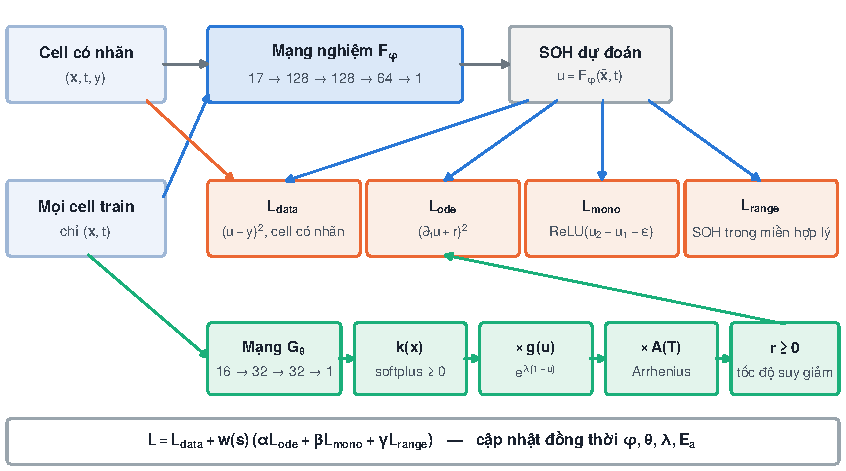
\includegraphics[width=\textwidth]{hinh/fig_thesis_arch.pdf}
\caption{Kiến trúc mô hình: mạng nghiệm dự đoán SOH, mạng tốc độ mô tả động học suy giảm; hai mạng gắn với
nhau qua các hàm mất mát vật lý.}\label{fig:arch}
\end{figure}

\subsection{Mạng nghiệm}

\begin{equation}
u = F_\varphi(\tilde{\mathbf{x}}, t), \qquad F_\varphi:\R^{17} \to \R,
\end{equation}
là perceptron nhiều lớp 17--128--128--64--1 với hàm kích hoạt SiLU.

\subsection{Động học suy giảm dạng xám}

\begin{equation}\label{eq:rate}
r(\tilde{\mathbf{x}}, u, T) =
\underbrace{\operatorname{softplus}\big(G_\theta(\tilde{\mathbf{x}})\big)}_{k(\mathbf{x})}\;
\underbrace{e^{\lambda\,\operatorname{clip}(1-u,\,-0{,}5,\,1)}}_{g(u)}\;
\underbrace{e^{-\frac{E_a}{R_g}\left(\frac{1}{T}-\frac{1}{T_\text{ref}}\right)}}_{A(T)},
\end{equation}
với $G_\theta$ là perceptron 16--32--32--1, $\lambda = \operatorname{softplus}(\lambda_\text{raw})$,
$E_a = 10^4 \operatorname{softplus}(e_\text{raw})$\,J/mol, $R_g = 8{,}314$\,J/(mol·K), $T_\text{ref} = 298{,}15$\,K.
Thừa số $k$ là tốc độ cơ sở phụ thuộc trạng thái điện hoá (thể hiện qua đặc trưng sạc), $g$ làm suy giảm tăng
nhanh khi SOH thấp (hiện tượng đầu gối), $A$ là hệ số Arrhenius. Phương trình mà mạng nghiệm phải thoả:
\begin{equation}\label{eq:ode}
\frac{\partial u}{\partial t} = -\,r(\tilde{\mathbf{x}}, u, T).
\end{equation}

\subsection{Hàm mất mát}

Với cặp chu kỳ $(n_1, n_2)$ của cùng một cell, $n_2 \ge n_1 + h$, $h \sim \mathcal{U}\{5,\dots,50\}$, ký hiệu
$u_i = F_\varphi(\tilde{\mathbf{x}}_{n_i}, t_{n_i})$:
\begin{align}
\mathcal{L}_\text{data} &= \tfrac{1}{B}\textstyle\sum (u - y)^2 && \text{(chỉ chu kỳ có nhãn)},\\
\mathcal{L}_\text{ode} &= \tfrac{1}{B}\textstyle\sum \big(\partial_t u_1 + r(\tilde{\mathbf{x}}_{n_1}, u_1, T)\big)^2, \\
\mathcal{L}_\text{mono} &= \tfrac{1}{B}\textstyle\sum \operatorname{ReLU}(u_2 - u_1 - \varepsilon), && \varepsilon = 0{,}002,\\
\mathcal{L}_\text{range} &= \tfrac{1}{B}\textstyle\sum \big[\operatorname{ReLU}(u_1 - 1{,}15) + \operatorname{ReLU}(0{,}4 - u_1)\notag\\
&\qquad\qquad + \mathbb{1}_\text{đầu}\big(\operatorname{ReLU}(u_1 - 1{,}10) + \operatorname{ReLU}(0{,}85 - u_1)\big)\big],
\end{align}
\begin{equation}
\mathcal{L} = \mathcal{L}_\text{data} + w(s)\big(\alpha\mathcal{L}_\text{ode} + \beta\mathcal{L}_\text{mono}
+ \gamma\mathcal{L}_\text{range}\big), \qquad w(s) = \min\big(1, s/(0{,}2S)\big),
\end{equation}
với $\alpha = 0{,}02$, $\beta = 0{,}5$, $\gamma = 1$, $S = 4000$ bước. $\mathbb{1}_\text{đầu} = 1$ nếu $n_1$ là
chu kỳ đầu của cell. Đạo hàm $\partial_t u$ tính bằng vi phân tự động.

\subsection{Cơ chế bán giám sát}

PINN-semi lấy một nửa số cặp chu kỳ từ cell có nhãn và một nửa từ cell không nhãn. Ba loss vật lý không chứa
$y$ (Mệnh đề~\ref{md:labelfree}), nên gradient của chúng theo $\varphi$ trên cell không nhãn là tín hiệu học
thật sự: mạng nghiệm bị buộc phải cho quỹ đạo hợp lý vật lý trên chính những cell mà nó sẽ phải tổng quát tới.

\subsection{Phần vật lý nằm ở đâu}\label{sec:wherephys}

Mạng nghiệm $F_\varphi$ tự nó là một perceptron nhiều lớp bình thường, giống hệt MLP đối chứng. Điều làm mô hình
trở thành PINN nằm ở hàm mất mát và ở các điểm mà hàm mất mát được tính, không nằm ở kiến trúc mạng hay ở bước
suy luận. Vật lý ở đây là vật lý ở mức hiện tượng: những quy luật định tính đã biết về lão hoá pin (dung lượng
không tự hồi phục, suy giảm nhanh dần khi pin già, phản ứng phụ tăng theo nhiệt độ), được viết thành phương trình
và bất đẳng thức. Đồ án không giải mô hình điện hoá chi tiết (P2D, mô hình hạt đơn) và không mô hình hoá đặc
trưng sạc bằng phương trình nào. Bảng~\ref{tab:physmap} nối từng hiểu biết vật lý với thành phần tương ứng.

\begin{table}[!htbp]\centering\small
\caption{Hiểu biết vật lý và thành phần mô hình tương ứng.}\label{tab:physmap}
\begin{tabularx}{\textwidth}{>{\raggedright}p{3.6cm}>{\raggedright}p{3.4cm}>{\raggedright}X c}
\toprule
Hiểu biết vật lý & Biểu diễn & Tác động vào đâu & Cần nhãn \\
\midrule
Dung lượng không tăng theo thời gian vận hành & $\partial u/\partial t = -r$, $r \ge 0$ & đạo hàm riêng
$\partial F_\varphi/\partial t$ tại điểm $(\tilde{\mathbf{x}}_{n_1}, t_{n_1})$, qua $\mathcal{L}_\text{ode}$ & không \\
Quỹ đạo SOH thực tế không tăng (cho phép hồi phục nhỏ $\varepsilon$) & $u_2 \le u_1 + \varepsilon$ & cặp chu kỳ
$(n_1, n_2)$ thật của cùng cell, qua $\mathcal{L}_\text{mono}$ & không \\
Suy giảm nhanh dần khi pin già (đầu gối) & $g(u) = e^{\lambda(1-u)}$ & thừa số trong $r$ & không \\
Phản ứng phụ tăng theo nhiệt độ & $A(T)$ dạng Arrhenius & thừa số trong $r$ & không \\
SOH nằm trong miền hợp lý, cell mới gần 1 & các hàm ReLU chặn & giá trị $u_1$, qua $\mathcal{L}_\text{range}$ & không \\
Dung lượng đo được & $(u - y)^2$ & chu kỳ có nhãn, qua $\mathcal{L}_\text{data}$ & có \\
\bottomrule
\end{tabularx}
\end{table}

Có ba điểm cần phân biệt. Thứ nhất, các ràng buộc được tính tại \emph{điểm collocation}: mọi chu kỳ của mọi cell
train, kể cả cell chưa đo dung lượng, ghép thành cặp $(n_1, n_2)$; đây là chỗ dữ liệu không nhãn đi vào mô hình.
Thứ hai, $\mathcal{L}_\text{ode}$ ràng buộc đạo hàm riêng theo $t$ khi giữ nguyên đặc trưng sạc, còn
$\mathcal{L}_\text{mono}$ ràng buộc tổng biến thiên dọc quỹ đạo thật, nơi cả $\mathbf{x}$ lẫn $t$ cùng đổi; hai
ràng buộc này tác động vào hai hướng khác nhau của hàm $F_\varphi$, và Mục~\ref{sec:physcheck} đo riêng từng hướng.
Thứ ba, khi suy luận chỉ dùng $F_\varphi$: vật lý định hình hàm được học, chứ không tham gia vào việc tính dự đoán.

\subsection{Tính chất của mô hình}

\begin{menhde}[Tốc độ suy giảm không âm]\label{md:rate}
Với mọi tham số $\theta, \lambda_\text{raw}, e_\text{raw}$ và mọi $(\tilde{\mathbf{x}}, u, T)$, $T > 0$:
$r(\tilde{\mathbf{x}}, u, T) \ge 0$. Do đó mọi nghiệm của \eqref{eq:ode} không tăng theo $t$.
\end{menhde}
\begin{proof}
$\operatorname{softplus}(z) = \ln(1+e^z) > 0$ với mọi $z$ thực vì $1 + e^z > 1$. Hai thừa số còn lại là hàm
mũ của số thực nên dương. Tích của ba số dương là dương; trong số học dấu phẩy động, softplus có thể tràn
dưới về $0$ nên phát biểu đúng là $r \ge 0$. Khi đó $\partial u/\partial t = -r \le 0$.
\end{proof}

\begin{menhde}[Loss vật lý không dùng nhãn]\label{md:labelfree}
$\mathcal{L}_\text{ode}$, $\mathcal{L}_\text{mono}$, $\mathcal{L}_\text{range}$ chỉ phụ thuộc đặc trưng và thời
điểm của cặp chu kỳ ($\tilde{\mathbf{x}}_{n_i}$, $t_{n_i}$), nhiệt độ $T$ và tham số
$(\varphi, \theta, \lambda, E_a)$; không phụ thuộc $y$. Vì vậy chúng tính được trên mọi cell chỉ có dữ liệu sạc.
\end{menhde}
\begin{proof}
Trực tiếp từ định nghĩa: không biểu thức nào chứa $y$; $\partial_t u_1$ là đạo hàm của $F_\varphi$ theo đầu vào
$t$, không qua nhãn.
\end{proof}

\begin{menhde}[Tập không của loss đơn điệu]\label{md:mono}
$\mathcal{L}_\text{mono} = 0$ khi và chỉ khi $u_2 \le u_1 + \varepsilon$ với mọi cặp trong batch; khi vi phạm,
gradient theo $u_2 - u_1$ bằng $1/B$ cho mỗi cặp vi phạm, không phụ thuộc mức vi phạm.
\end{menhde}
\begin{proof}
$\operatorname{ReLU}(z) \ge 0$ và bằng $0$ khi và chỉ khi $z \le 0$, nên tổng các số hạng không âm bằng $0$ khi
và chỉ khi từng số hạng bằng $0$. Đạo hàm của $\operatorname{ReLU}$ bằng $1$ trên $z > 0$.
\end{proof}

\begin{menhde}[Dạng tích phân của phần dư]\label{md:euler}
Nếu $u$ thoả \eqref{eq:ode} dọc một quỹ đạo và $r$ khả vi liên tục theo $t$ trên $[t_1, t_2]$, thì phần dư dạng
Euler $\rho = u_2 - u_1 + r_1\Delta t$ thoả $|\rho| \le \tfrac12 \max|\dot r|\,\Delta t^2$.
\end{menhde}
\begin{proof}
$u_2 - u_1 = -\int_{t_1}^{t_2} r(s)\,ds = -r_1\Delta t - \int_{t_1}^{t_2}(r(s) - r_1)\,ds$, và
$|r(s) - r_1| \le \max|\dot r|\,(s - t_1)$. Lấy tích phân được cận $\tfrac12\max|\dot r|\Delta t^2$.
\end{proof}

Mệnh đề~\ref{md:euler} cho thấy dạng Euler dọc quỹ đạo và dạng đạo hàm riêng $\partial_t u$ là hai ràng buộc
khác nhau: dạng thứ nhất ràng buộc tổng biến thiên dọc chuỗi chu kỳ thực (khi đặc trưng $\mathbf{x}$ cũng thay
đổi), dạng thứ hai ràng buộc đạo hàm theo $t$ khi giữ $\mathbf{x}$ cố định. Cả hai được so sánh ở
Chương~\ref{ch:ketqua}.

\section{Mô hình kết hợp PINN-lai}\label{sec:pinnlai_m}
Chương~\ref{ch:ketqua} sẽ cho thấy sai số còn lại của PINN-semi chủ yếu là lệch mức theo từng cell, và GBDT có sai số thấp nhất khi có đủ nhãn. Mục này mô tả các thành phần được xem xét để cải tiến mô hình và mô hình kết hợp được chọn.

\subsection{Các thành phần được xem xét}\label{sec:candidates}

Sáu thành phần được xem xét, mỗi thành phần dựa trên một kết quả đã công bố hoặc một quan sát ở Chương~\ref{ch:ketqua}; Mục~\ref{sec:devproto} chọn trong số đó chỉ bằng tập validation.

\paragraph{Nhóm mạng.} Huấn luyện $M = 3$ mạng PINN-semi giống hệt nhau, chỉ khác hạt giống khởi tạo và thứ tự lấy
batch, rồi lấy trung bình $\bar F = \frac{1}{M}\sum_m F^{(m)}$~\cite{lakshminarayanan2017}. Cả ba mạng dùng đúng
cùng cách chia và cùng tập cell có nhãn, nên không có nhãn nào được thêm vào.

\paragraph{Kết hợp với GBDT.} Lấy trung bình dự đoán của nhóm mạng và của GBDT, $\hat y = \omega \bar F + (1-\omega) g$.
Đây là dạng đơn giản nhất của kết hợp mô hình khác loại~\cite{wolpert1992}. Lý do để kỳ vọng nó giúp là hai mô hình
có thiên lệch quy nạp khác hẳn nhau: cây quyết định học tốt các hàm không trơn trên dữ liệu bảng~\cite{grinsztajn2022},
còn PINN-semi dùng được cell không nhãn và cho quỹ đạo trơn, gần đơn điệu.

\paragraph{Bộ lọc quỹ đạo.} Vật lý cũng có thể được đưa vào ở bước suy luận chứ không chỉ khi huấn luyện. Tại chu kỳ
$n$ của một cell, lấy $w$ dự đoán gần nhất $\hat y_{n-w+1}, \dots, \hat y_n$, khớp một đường thẳng bằng bình phương
tối thiểu~\cite{cleveland1979} với ràng buộc độ dốc không dương, rồi lấy giá trị đường thẳng tại $n$:
\begin{equation}\label{eq:trend}
\tilde y_n = \bar y + \min(0, \hat\beta)\,(t_n - \bar t), \qquad
\hat\beta = \frac{\sum_i (t_i - \bar t)(\hat y_i - \bar y)}{\sum_i (t_i - \bar t)^2},
\end{equation}
với $\bar t, \bar y$ là trung bình trên cửa sổ. Bộ lọc chỉ dùng dự đoán của các chu kỳ đã qua, không dùng nhãn,
nên chạy được trực tuyến. Một lựa chọn tự nhiên khác là hồi quy đơn điệu~\cite{barlow1972} trên toàn bộ quá khứ,
nhưng Mệnh đề~\ref{prop:filter} cho thấy nó lệch xuống.

\paragraph{Ba hướng khác.} Chưng cất từ GBDT dùng dự đoán của GBDT trên cell không nhãn làm mục tiêu mềm cho
mạng~\cite{hinton2015,lee2013}, thêm số hạng $\lambda_\text{KD}\,\overline{(F_\varphi - g)^2}$. Ràng buộc vật lý mạnh
hơn tăng trọng số đơn điệu lên $\beta = 2$, hoặc thêm phần dư Euler dọc quỹ đạo với hệ số $\alpha_E = 2$. Đặc trưng
tương đối nối thêm $(\mathbf{x}_n - \mathbf{x}_\text{ref})/|\mathbf{x}_\text{ref}|$ so với trung bình ba chu kỳ đầu
của cell, theo tinh thần của $\Delta Q(V)$ trong~\cite{severson2019}.

\subsection{Mô hình PINN-lai}\label{sec:pinnlai}

Mô hình cải tiến, gọi là PINN-lai, gồm ba bước:
\begin{align}
\bar F(\mathbf{x}, t) &= \tfrac{1}{3}\textstyle\sum_{m=1}^{3} F_{\varphi_m}(\tilde{\mathbf{x}}, t), \label{eq:lai1}\\
\hat y_n &= \tfrac{1}{2}\,\bar F(\mathbf{x}_n, t_n) + \tfrac{1}{2}\,g(\mathbf{x}_n, t_n), \label{eq:lai2}\\
\tilde y_n &= \text{bộ lọc \eqref{eq:trend} với } w = 10 \text{ trên } \hat y_{n-9}, \dots, \hat y_n, \label{eq:lai3}
\end{align}
trong đó $F_{\varphi_m}$ là ba mạng PINN-semi cấu hình như Mục~\ref{sec:pinn} và $g$ là GBDT như
Mục~\ref{sec:baselines}, cùng học trên đúng các cell
có nhãn của fold. Huấn luyện tốn gấp ba PINN-semi cộng một GBDT; suy luận vẫn chỉ cần đặc trưng sạc của chu kỳ hiện
tại và chín dự đoán trước đó của chính cell.

\begin{menhde}\label{prop:filter}
Xét một cửa sổ $w$ điểm cách đều.
(i) Nếu $\hat y_i = a - c\,t_i$ với $c \ge 0$ thì $\tilde y_n = \hat y_n$: bộ lọc không làm lệch một quỹ đạo giảm
tuyến tính.
(ii) Nếu $\hat y_i = a - c\,t_i + \epsilon_i$ với $\epsilon_i$ độc lập, kỳ vọng 0, phương sai $\sigma^2$, và ràng
buộc độ dốc không kích hoạt, thì $\tilde y_n$ không chệch và
$\operatorname{Var}(\tilde y_n) = \sigma^2\,\dfrac{2(2w-1)}{w(w+1)}$; với $w = 10$ là $0{,}345\,\sigma^2$.
(iii) Giá trị cuối của hồi quy đơn điệu giảm trên $\hat y_1, \dots, \hat y_n$ luôn không lớn hơn $\hat y_n$, nên
khi $\hat y$ có nhiễu nó lệch xuống.
(iv) Dãy $\tilde y_1, \tilde y_2, \dots$ không nhất thiết đơn điệu: ràng buộc chỉ đặt lên độ dốc trong từng cửa sổ, còn
hai chu kỳ liền nhau dùng hai cửa sổ khác nhau. Dãy
\begin{equation}\label{eq:mono}
m_1 = \tilde y_1, \qquad m_n = m_{n-1} + a\,\min(0,\ \tilde y_n - m_{n-1}), \quad 0 < a \le 1,
\end{equation}
thì luôn không tăng; $a = 1$ cho cực tiểu luỹ tiến của $\tilde y$.
\end{menhde}
\begin{proof}
(i) Đường thẳng khớp đúng dữ liệu, độ dốc $-c \le 0$ nên ràng buộc không tác động. (ii) Đây là phương sai của giá
trị dự đoán bình phương tối thiểu tại đầu mút: $\sigma^2\big(\frac{1}{w} + \frac{(t_n - \bar t)^2}{S_{tt}}\big)$
với $t_n - \bar t = \frac{w-1}{2}$ và $S_{tt} = \frac{w(w^2-1)}{12}$ khi bước bằng 1; rút gọn được biểu thức trên.
(iii) Với hồi quy đơn điệu giảm, giá trị tại điểm cuối bằng $\min_{j \le n}$ trung bình của $\hat y_j, \dots, \hat y_n$
\cite{barlow1972}; chọn $j = n$ cho thấy nó không vượt $\hat y_n$. (iv) Lấy $\hat y = (0{,}9;\ 0{,}9;\ 0{,}95)$, $w = 2$:
$\tilde y_2 = 0{,}9$, còn cửa sổ thứ ba có độ dốc dương bị chặn về 0 nên $\tilde y_3 = 0{,}925 > \tilde y_2$. Với
\eqref{eq:mono}, $m_n - m_{n-1} = a\min(0, \tilde y_n - m_{n-1}) \le 0$.
\end{proof}

\section{Đầu vào có lịch sử của cell}\label{sec:hist_m}

PINN-semi, MLP và GBDT đều dự đoán SOH ở chu kỳ $n$ chỉ từ 16 đặc trưng sạc của chính chu kỳ đó và chỉ số chu kỳ.
Đặc trưng của một chu kỳ có nhiễu đo, trong khi các chu kỳ liền trước mang thông tin về gần như cùng một trạng thái của
cell. Đồ án thêm lịch sử vào đầu vào bằng các đại lượng nhân quả, chỉ dùng chu kỳ $n$ và các chu kỳ trước của cùng
cell nên vẫn chạy trực tuyến được: trung bình trượt mũ
\begin{equation}\label{eq:ema}
\mathbf{z}^{(a)}_1 = \mathbf{x}_1, \qquad \mathbf{z}^{(a)}_n = a\,\mathbf{x}_n + (1-a)\,\mathbf{z}^{(a)}_{n-1},
\end{equation}
nhớ khoảng $1/a$ chu kỳ, và độ dốc bình phương tối thiểu của từng đặc trưng trên 20 chu kỳ gần nhất. Bốn dạng được
thử: chỉ $\mathbf{z}^{(0{,}3)}$ thay cho $\mathbf{x}$; $\mathbf{x}$ nối với $\mathbf{z}^{(0{,}1)}$; $\mathbf{x}$ nối
với $\mathbf{z}^{(0{,}3)}, \mathbf{z}^{(0{,}1)}, \mathbf{z}^{(0{,}03)}$; và $\mathbf{x}$ nối với $\mathbf{z}^{(0{,}1)},
\mathbf{z}^{(0{,}03)}$ cùng độ dốc. GBDT thử thêm $\mathbf{x}$ nối với độ dốc, và $\mathbf{x}, \mathbf{z}^{(0{,}1)}$ nối
với độ lệch của $\mathbf{x}$ so với trung bình 5 chu kỳ đầu của cell. Đây là một lớp hồi quy tuyến tính với hệ số cố định, cùng ý tưởng với mô hình không
gian trạng thái của SambaMixer~\cite{olalde2024samba} nhưng không học hệ số. Mọi mô hình dùng được cùng đầu vào, nên
phép so sánh tách được tác động của lịch sử khỏi tác động của vật lý. Với mỗi bộ và mỗi loại mô hình, dạng lịch sử được
chọn trên tập validation và chỉ được giữ khi nó giảm MAE validation ít nhất 2\,\%; nếu không, mô hình dùng đặc trưng
gốc. PINN-lai có lịch sử dùng đúng công thức \eqref{eq:lai1}--\eqref{eq:lai3} với ba PINN-semi và GBDT đã chọn cho bộ.

\section{Dự báo SOH tương lai, dung lượng còn lại và RUL}\label{sec:forecast_m}

Mô hình ở các mục trên trả lời câu hỏi pin đang ở đâu. Mục này mở rộng sang câu hỏi pin sẽ đi tới đâu: tại chu kỳ
gốc $k$ của một cell, dự báo SOH ở mọi chu kỳ $k + h$, $h > 0$, rồi suy ra dung lượng còn lại
$\hat Q(k+h) = \hat y(k+h)\,C_\text{dđ}$ (Ah, $C_\text{dđ}$ là dung lượng danh định) và
$\text{RUL}_k = \min\{h : \hat y(k+h) \le \tau\}$.

\paragraph{Thông tin tại gốc.} Bộ dự báo chỉ dùng các chu kỳ $\le k$: đặc trưng sạc $\mathbf{x}_1, \dots,
\mathbf{x}_k$ và một chuỗi SOH lịch sử $s_1, \dots, s_k$. Chuỗi lịch sử có hai nguồn, ứng với hai kịch bản: dung lượng
đo thật, khi BMS có đo dung lượng định kỳ; hoặc SOH do PINN-lai ước lượng từ đặc trưng sạc, khi cell không được đo
dung lượng lần nào. Từ đó tạo vectơ $\mathbf{z}_k$ gồm 23 thành phần: mức hiện tại $\ell_k$ (bộ lọc
\eqref{eq:trend} với $w = 10$ áp lên $s$), độ dốc bình phương tối thiểu trên 30 và 100 chu kỳ gần nhất, mức ban đầu $\ell_0$ (trung
bình 5 chu kỳ đầu) và độ giảm $\ell_0 - \ell_k$, $k/1000$, $1000/T$, cùng trung bình 16 đặc trưng sạc đã chuẩn hoá
trên 10 chu kỳ gần nhất.

\paragraph{Nghiệm đóng của động học xám.} Mạng tốc độ ở Mục~\ref{sec:pinn} mô tả
$\partial u/\partial t = -r(\mathbf{x})\,e^{\lambda(1-u)}A(T)$. Đặc trưng sạc của các chu kỳ tương lai chưa biết, nên
trong tầm dự báo coi $r(\mathbf{x})A(T)$ là hằng số. Đặt $v = 1 - u$, phương trình trở thành
$\mathrm{d}v/\mathrm{d}N = a_0 e^{\lambda v}$; tích phân từ gốc $k$ cho
\begin{equation}\label{eq:fcdrop}
  \Delta v(h) = v(k+h) - v(k) = -\frac{1}{\lambda}\ln\bigl(1 - \lambda a h\bigr),
\end{equation}
trong đó $a$ là tốc độ suy giảm tại gốc (trên 1000 chu kỳ) và $h$ tính bằng nghìn chu kỳ. Khi $\lambda > 0$ suy giảm
tăng tốc và đường cong dốc đứng khi $h$ tiến tới $1/(\lambda a)$, đúng hình dạng của điểm đầu gối; khi $\lambda < 0$ suy
giảm chậm dần; khi $\lambda \to 0$ ta có $\Delta v = a h$. Với mọi $a \ge 0$, $\Delta v$ không âm và không giảm theo
$h$, nên dự báo luôn đơn điệu mà không cần số hạng phạt. RUL cũng có dạng đóng:
\begin{equation}\label{eq:fcrul}
  h_\tau = \frac{1 - e^{-\lambda(\ell_k - \tau)}}{\lambda a}.
\end{equation}

\paragraph{PINN-dự báo.} Một mạng hai lớp ẩn 64 nút nhận $\mathbf{z}_k$ và trả $(a, \lambda)$, với $a$ qua hàm
softplus và $\lambda = 80\tanh(\cdot/80)$; dự báo là $\hat y(k+h) = \ell_k - \Delta v(h; a, \lambda)$, giới hạn trong
$[0{,}40;\,1{,}15]$. Hàm mất mát là sai số bình phương giữa $\hat y(k+h)$ và SOH đo trên các cặp (gốc, tầm) lấy từ
cell train: mỗi cell cho 40 gốc cách đều, mỗi gốc 40 điểm đích cách đều trong phần đời còn lại, nên các cell có trọng
số gần bằng nhau bất kể độ dài. Khác với PINN-semi, vật lý ở đây là ràng buộc cứng: nghiệm của phương trình động học
chính là lớp đầu ra. Ba thành viên với hạt giống khác nhau được lấy trung bình, dừng sớm theo MAE trên cell
validation.

\paragraph{GBDT trực tiếp và mô hình kết hợp.} GBDT học ánh xạ $(\mathbf{z}_k, h) \mapsto \ell_k - y(k+h)$ trên cùng
các cặp, với ràng buộc đơn điệu tăng theo $h$, cùng cấu hình và cách chọn số cây như GBDT đối chứng. Mô hình kết hợp
lấy trung bình hai dự báo, theo đúng lý do của PINN-lai: GBDT nội suy tốt trong miền tầm dự báo đã thấy nhưng đi
ngang bên ngoài miền đó, còn PINN-dự báo ngoại suy theo dạng hàm của động học.

\paragraph{Mô hình đối chứng.} (i) Giữ nguyên: $\hat y(k+h) = \ell_k$. (ii) Ngoại suy tuyến tính theo độ dốc 100 chu
kỳ gần nhất, chặn để không dương. (iii) Khớp vật lý theo cell: khớp \eqref{eq:fcdrop} với ba tham số
$(u_0, a_0, \lambda)$ lên nửa sau lịch sử của chính cell, có phạt nhẹ $\lambda$, rồi ngoại suy, đại diện cho nhóm
mô hình thực nghiệm khớp theo từng cell~\cite{he2011}.

\paragraph{Xét hồi phục dung lượng.} Bản cải tiến tách lịch sử tại gốc thành ba phần, chỉ dùng 60 chu kỳ gần nhất:
(i) xu thế, là đường thẳng khớp bằng hồi quy Huber nên vài điểm hồi phục không kéo lệch được mức và độ dốc;
(ii) dao động đều, chu kỳ $P \in [2{,}2;\,15]$ với hai hài trên phần dư, chỉ giữ khi giải thích được ít nhất 60\,\%
phương sai trên cả cửa sổ lẫn từng nửa cửa sổ; (iii) phần hồi phục hiện tại $e_k$, phần dư của chu kỳ cuối sau khi trừ hai
phần trên, co về 0 một khoảng bằng hai lần mức nhiễu cục bộ để nhiễu đo không bị coi là hồi phục. Dự báo trở thành
\begin{equation}\label{eq:fcrec}
  \hat y(k+h) = \ell_k + e_k\,g(h) - \Delta v(h; a, \lambda) + p_k(h), \qquad g(h) = \rho + (1 - \rho)\,e^{-h/\tau_r},
\end{equation}
trong đó $\ell_k$ là giá trị xu thế tại gốc, $\Delta v$ là nghiệm đóng \eqref{eq:fcdrop} chỉ cho phần suy giảm không
thuận nghịch, $p_k(h)$ là dao động ngoại suy, $\rho$ là phần hồi phục được giữ lại và $\tau_r$ là thời gian tắt của phần
còn lại. Cặp $(\rho, \tau_r)$ được ước lượng trực tiếp trên cell train của từng fold: tại mỗi lần hồi phục (SOH đo vượt
trung vị năm chu kỳ trước đó quá 0,004), phần lệch của SOH so với xu thế cộng dao động trong 30 chu kỳ sau được khớp
bằng $e_k\,g(h)$, dò lưới $\rho \in \{0; 0{,}1; \dots; 1\}$ và $\tau_r \in \{0{,}5; 1; \dots; 40\}$ chu kỳ; bộ có dưới năm
lần hồi phục nhận $\rho = 0$. GBDT học phần giảm của xu thế sau khi trừ hai thành phần thuận nghịch, với trọng số trong
mô hình kết hợp tăng tuyến tính từ 0 tại $h = 0$ tới $\tfrac{1}{2}$ tại $h = 0{,}1L$. Các lựa chọn này được chốt trên cell
validation của lần lặp đầu tiên, trước khi chạy trên test.

\paragraph{Khoảng dự báo.} Sai số có dấu (thật trừ dự báo) của mô hình kết hợp trên cell validation được chia theo
tầm tương đối $h/L$ ($L$ là trung vị số chu kỳ của bộ, các nhóm cận 0,05; 0,1; 0,25; 0,5; 1); cộng phân vị 5\,\% và
95\,\% của mỗi nhóm vào dự báo cho khoảng 90\,\%. Cận dưới và cận trên của RUL là lúc biên dưới và biên trên của
khoảng cắt ngưỡng $\tau$.
\section{Học và cập nhật với vài lần đo dung lượng}\label{sec:kalman_m}

Nhãn của bài toán là dung lượng đo bằng một lần xả đầy ở điều kiện chuẩn, nên chi phí nhãn nằm ở số lần đo chứ không ở
số cell. Giao thức chính đếm nhãn theo cell: 30\,\% cell có nhãn nghĩa là mọi chu kỳ của 30\,\% số cell đều được đo.
Mục này mô tả cách mô hình dùng một số ít lần đo rải trên nhiều cell, ở hai thời điểm: khi huấn luyện và khi dùng mô
hình cho một cell mới.

\paragraph{Nhãn thưa khi huấn luyện.} Mỗi cell train được đo dung lượng ở chu kỳ đầu, sau mỗi $qL$ chu kỳ ($L$ là trung
vị số chu kỳ của các cell train) và ở chu kỳ cuối của thử nghiệm; các chu kỳ còn lại chỉ có đặc trưng sạc. Với PINN-semi, $\mathcal{L}_\text{data}$ chỉ tính trên các chu kỳ được
đo, còn ba loss vật lý vẫn tính trên cặp chu kỳ của mọi hàng của mọi cell: ràng buộc đơn điệu và phần dư động học nối
các lần đo với nhau, nên thông tin của một lần đo lan sang các chu kỳ lân cận mà không cần nhãn ở đó. GBDT không có cơ
chế này; với nó, SOH ở các chu kỳ giữa hai lần đo được lấy theo nội suy tuyến tính trước khi học (lan nhãn). PINN-lai
ở chế độ này giữ nguyên công thức \eqref{eq:lai1}--\eqref{eq:lai3}, với ba mạng PINN-semi học từ nhãn thưa và GBDT học
nhãn nội suy.

\paragraph{Cập nhật theo cell khi dùng.} Sai số còn lại của PINN-lai chủ yếu là độ lệch mức riêng của từng cell
(Mục~\ref{sec:improve}), không thể sửa nếu không có thông tin nào về chính cell. Khi cell mới cũng được đo vài lần (lúc
nhận pin, khi bảo dưỡng định kỳ), gọi $p_n$ là SOH do mô hình ước lượng ở chu kỳ $n$ và $y_n$ là SOH đo được; sai số
được mô hình hoá
\begin{equation}\label{eq:kf}
  y_n - p_n = b_n + \varepsilon_n,\qquad
  b_{n'} - \mu_0 = e^{-(n'-n)/\ell}\,(b_n - \mu_0) + \eta,\qquad
  \operatorname{Var}\varepsilon = R,\ \operatorname{Var} b = P_0,
\end{equation}
tức độ lệch $b_n$ của cell trôi chậm và hồi quy về trung bình $\mu_0$ với độ dài tương quan $\ell$ (quá trình
Ornstein--Uhlenbeck), còn $\varepsilon_n$ là nhiễu nhanh. Bộ lọc Kalman cập nhật $b$ mỗi khi có một lần đo. Ước lượng hiệu chỉnh là $p_n + \hat b_n$, với $\hat b_n$ chỉ
dùng các lần đo ở chu kỳ $\le n$, kèm khoảng 90\,\% $\pm 1{,}645\sqrt{\hat P_n + R}$. Bốn tham số lấy trên cell validation
của chính fold: $\mu_0$ là sai số trung bình, $R$ là nửa phương sai của sai phân bậc một, $P_0$ là phần phương sai còn
lại, $\ell$ chọn trên lưới theo MAE riêng cho từng lịch đo. Với dự báo, đường dự báo của mô hình kết hợp có xét hồi phục
được cộng thêm độ lệch hậu nghiệm tại gốc, trôi dần về $\mu_0$ theo \eqref{eq:kf} trong tầm dự báo.
\section{Các mô hình đối chứng}\label{sec:baselines}

Mọi mô hình ở Bảng~\ref{tab:models} dùng cùng đặc trưng $[\tilde{\mathbf{x}}, t]$ (mô hình chuỗi nhận thêm các chu kỳ trước của chính cell), cùng cách chia, cùng tập cell có nhãn và cùng
normaliser.

\begin{table}[!htbp]\centering\small
\caption{Các mô hình được so sánh.}\label{tab:models}
\begin{tabularx}{\textwidth}{l>{\raggedright}p{3.2cm}>{\raggedright\arraybackslash}X}
\toprule
Mô hình & Nhóm & Mô tả \\
\midrule
Ridge & học có nhãn & hồi quy tuyến tính chuẩn hoá L2; $\alpha \in \{10^{-3},\dots,10^{3}\}$ chọn theo validation\\
GPR & học có nhãn & hồi quy Gauss~\cite{rasmussen2006}, nhân RBF + nhiễu trắng, 1\,500 điểm có nhãn chọn ngẫu nhiên\\
GBDT & học có nhãn & gradient boosting trên cây~\cite{friedman2001}, dạng histogram~\cite{ke2017}; số cây chọn theo validation\\
MLP & học có nhãn & cùng kiến trúc với mạng nghiệm, chỉ $\mathcal{L}_\text{data}$\\
CNN & học có nhãn, chuỗi & tích chập nhân quả trên cửa sổ $L$ chu kỳ gần nhất\\
LSTM & học có nhãn, chuỗi & một lớp LSTM trên cùng cửa sổ\\
Transformer & học có nhãn, chuỗi & một lớp encoder tự chú ý, mã hoá vị trí hình sin\\
PINN-sup & vật lý trên cell có nhãn & như PINN-semi nhưng loss vật lý chỉ tính trên cell có nhãn\\
PINN hộp đen & vật lý, bán giám sát & động học dạng PINN4SOH~\cite{wang2024}: $u_t = G(\mathbf{x}, t, u, u_\mathbf{x}, u_t)$, cùng loss không nhãn\\
PINN-semi & vật lý, bán giám sát & mô hình đề xuất\\
\bottomrule
\end{tabularx}
\end{table}

Hai biến thể cắt bỏ dùng để tách nguồn gốc lợi ích: \emph{chỉ đơn điệu} ($\alpha = \gamma = 0$) và
\emph{PINN-semi dạng Euler} (dùng phần dư dọc quỹ đạo thay cho $\partial_t u$, $\alpha = 2$).


\paragraph{CNN, LSTM, Transformer.} Đầu vào ở chu kỳ $n$ là cửa sổ nhân quả $L$ chu kỳ gần nhất của chính cell (16 đặc
trưng sạc đã chuẩn hoá và chỉ số chu kỳ; đầu cửa sổ lặp lại chu kỳ đầu khi cell chưa đủ $L$ chu kỳ), đầu ra là SOH ở
chu kỳ $n$, nên cả ba chạy trực tuyến như các mô hình khác. CNN có 32 kênh, kích thước 5, độ giãn 1 và 2 (vùng nhìn 13
chu kỳ); LSTM 32 nút ẩn; Transformer 32 chiều, 4 đầu chú ý. Cả ba chỉ học có nhãn với AdamW (tốc độ học $10^{-3}$),
batch 128, cắt gradient ở chuẩn 1, dừng sớm theo MAE trên cell validation. Độ dài cửa sổ chọn trên validation trong
$\{16, 48\}$: $L = 16$ cho CNN và Transformer; $L = 48$ cho LSTM.
\section{Cấu hình huấn luyện}

\begin{table}[!htbp]\centering\small
\caption{Cấu hình huấn luyện chung cho MLP và các biến thể PINN.}\label{tab:train}
\begin{tabularx}{\textwidth}{l>{\raggedright\arraybackslash}X}\toprule
Thành phần & Giá trị \\\midrule
Bộ tối ưu & AdamW~\cite{loshchilov2019}, tốc độ học $2\cdot10^{-3}$, weight decay $10^{-5}$ \\
Lịch tốc độ học & cosine, giảm về $10^{-4}$ trong 4\,000 bước \\
Batch & 512 điểm có nhãn; 512 cặp chu kỳ cho loss vật lý \\
Cắt gradient & chuẩn $L_2 \le 5$ \\
Dừng sớm & MAE trên validation mỗi 100 bước, dừng sau 12 lần không cải thiện, giữ trọng số tốt nhất \\
\bottomrule\end{tabularx}\end{table}

Ngoài cấu hình ở Bảng~\ref{tab:train}, trọng số vật lý ($\alpha, \beta$) và dạng phần dư được chọn trước theo MAE validation ở một thí nghiệm sơ bộ
và giữ cố định trong toàn bộ các thí nghiệm của báo cáo; không có siêu tham số nào được chọn theo tập test.

\chapter{Hiện thực hệ thống và thiết kế thí nghiệm}\label{ch:thietke}

Chương này mô tả cách hệ thống được hiện thực và cách đánh giá: chia dữ liệu theo đơn vị nào và thành bao nhiêu
phần, vì sao chọn đúng các con số đó, và làm sao bảo đảm không có thông tin của tập test lọt vào quá trình huấn
luyện.

\section{Kiến trúc hiện thực}\label{sec:impl}

Hệ thống được hiện thực bằng Python thành một đường ống năm khối (Hình~\ref{fig:pipeline}), chạy được từ dữ liệu thô
tới báo cáo bằng một lệnh và cho kết quả giống từng bit khi chạy lại.

\begin{enumerate}
\item Khối dữ liệu đọc dữ liệu đa định dạng của năm bộ (bảng CSV của bốn bộ chính, tệp MATLAB của NASA), trích 16 đặc
      trưng của đoạn sạc, lọc ngoại lai chỉ bằng dữ liệu quá khứ, chuẩn hoá bằng thống kê của cell train và lưu bộ đệm.
\item Khối mô hình gồm các mạng nơ-ron viết bằng PyTorch (MLP, CNN, LSTM, Transformer, PINN-semi, PINN-dự báo), các
      mô hình cổ điển của scikit-learn (Ridge, GPR, GBDT) và các bước hậu xử lý độc lập: bộ lọc quỹ đạo, khoảng dự đoán
      phù hợp, bộ lọc Kalman theo cell.
\item Khối thí nghiệm biểu diễn mỗi thí nghiệm bằng một danh sách lượt chạy (bộ dữ liệu, mô hình, mức nhãn, lần lặp,
      fold); bộ lập lịch chạy song song nhiều tiến trình một luồng, lượt dài trước, bỏ qua lượt đã có kết quả nên
      chạy tiếp được sau khi dừng, và ghi mỗi lượt thành một tệp có đủ cấu hình, chỉ số, dự đoán validation và test.
\item Khối phân tích chỉ đọc các tệp kết quả, không huấn luyện lại: tính chỉ số, kiểm định ghép cặp, chọn siêu tham số
      trên validation, vẽ hình.
\item Khối báo cáo sinh toàn bộ báo cáo này, mọi con số đọc từ kết quả phân tích. Một công cụ dòng lệnh nhận dữ liệu
      sạc của một cell và trả SOH ước lượng, dự báo SOH, dung lượng còn lại, RUL kèm hình quỹ đạo, làm bản mẫu cho giao
      diện của giai đoạn 2.
\end{enumerate}

Mọi thí nghiệm chạy trên CPU (Intel Xeon 2,1\,GHz, 4 lõi); phần mềm gồm Python 3.11, PyTorch, scikit-learn, NumPy,
SciPy, pandas và Matplotlib. Mỗi lượt dùng một luồng và hạt giống cố định; chạy lại 20 lượt mẫu trên máy khác cho dự
đoán trùng từng bit với kết quả báo cáo. Bảng~\ref{tab:exps} liệt kê các thí nghiệm và số lượt huấn luyện.

\begin{figure}[!htbp]\centering
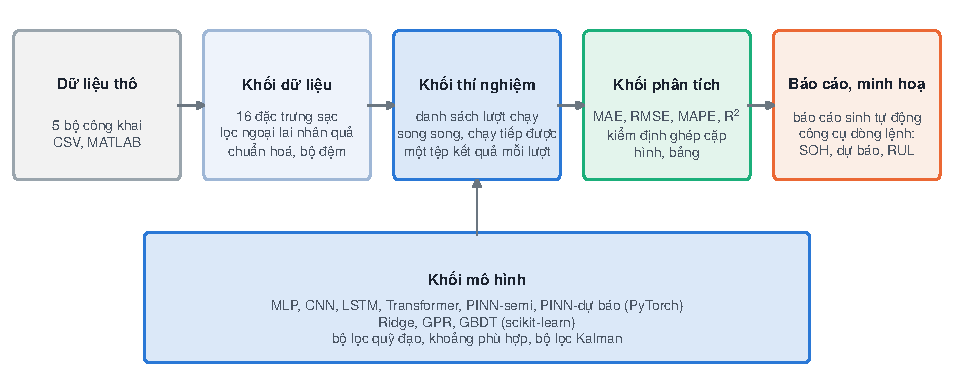
\includegraphics[width=\textwidth]{hinh/fig_thesis_pipeline.pdf}
\caption{Kiến trúc hiện thực: năm khối của hệ thống, từ dữ liệu thô tới báo cáo và công cụ minh hoạ.}\label{fig:pipeline}
\end{figure}

\begin{table}[!htbp]\centering\small
\caption{Các thí nghiệm và số lượt huấn luyện.}\label{tab:exps}
\begin{adjustbox}{max width=\textwidth}\begin{tabular}{llr}\toprule
Thí nghiệm & Nội dung & Lượt \\\midrule
Kiểm định chéo chính & MLP, PINN-semi ở 4 mức; PINN-sup, 2 biến thể cắt bỏ ở 30\,\% & 1.100 \\
Đối chứng học có nhãn & Ridge, GPR, GBDT ở 4 mức nhãn & 1.200 \\
Mở rộng biến thể vật lý & PINN-sup ở 10, 50\,\%; PINN hộp đen ở 4 mức & 600 \\
Kiểm toán rò rỉ & 4 cách chia/chuẩn hoá sai, MLP 70\,\% nhãn, 2 lần lặp & 160 \\
Cải tiến mô hình (Mục~\ref{sec:improve}) & 9 hướng trên validation; PINN-lai, 3 lần lặp, 4 mức nhãn & 1.680 \\
Dự báo SOH tương lai và RUL & GBDT + 3 PINN-dự báo mỗi fold, 5 fold × 3 lần lặp × 4 bộ & 75 \\
Dự báo có xét hồi phục & cùng fold với E22, thêm bộ NASA; học lại cả mô hình E22 để so ghép cặp & 75 \\
Bộ NASA & 2 bộ đặc trưng × 2 mức nhãn × 15 fold; cách chia của SambaMixer, 3 hạt giống & 330 \\
Tham số vật lý & NASA, TJU: trọng số ODE, ràng buộc Euler, giá trị khởi tạo; 70\,\% nhãn & 100 \\
So với PINN4SOH & đúng cách chia của bài, 39 nhóm (đầy đủ và ít mẫu) × 2 cách tiền xử lý × 3 hạt giống & 1.002 \\
Ngân sách đo & đo thưa mọi cell train, 4 lịch đo × 4 bộ × 5 fold × 3 lần lặp & 1.560 \\
Đầu vào có lịch sử & chọn dạng trên validation; PINN-semi, MLP, GBDT có lịch sử, 3 lần lặp × 5 fold & 1.416 \\
CNN, LSTM, Transformer & chọn cửa sổ trên validation; 4 mức nhãn × 4 bộ × 3 lần lặp × 5 fold; NASA & 1.158 \\
\textbf{Tổng} &  & \textbf{10.456} \\
\bottomrule\end{tabular}\end{adjustbox}\end{table}

\section{Các yêu cầu đối với giao thức}

\begin{enumerate}[label=\textbf{Y\arabic*.}]
\item \emph{Không rò rỉ}: mô hình và mọi bước tiền xử lý không được dùng bất kỳ thông tin nào của cell test.
\item \emph{Phủ hết dữ liệu}: mỗi cell đều phải được dùng làm test, để kết quả không phụ thuộc vào việc chọn may
      rủi một nhóm cell test.
\item \emph{Phủ hết điều kiện thí nghiệm}: mỗi fold phải có cell của mọi chế độ thí nghiệm, để không có fold
      nào chỉ kiểm tra trên một chế độ lạ.
\item \emph{Đủ nhãn ở mức thấp nhất}: ở 10\,\% nhãn, bộ nhỏ nhất (XJTU, 55 cell) vẫn phải có vài cell có nhãn.
\item \emph{Đủ cell validation} để dừng sớm và chọn siêu tham số ổn định.
\item \emph{Đủ chỗ cho mức nhãn cao nhất}: tập train phải chứa được 70\,\% số cell có nhãn.
\item \emph{Ước lượng ổn định}: đủ số lần lặp để kết quả không phụ thuộc một cách xáo ngẫu nhiên.
\item \emph{Ghép cặp}: mọi mô hình dùng đúng cùng các tập cell, để so sánh được theo từng cell.
\end{enumerate}

\section{Đơn vị chia: cell, không phải chu kỳ}\label{sec:unit}

Các chu kỳ liên tiếp của một cell gần như giống nhau: SOH chỉ thay đổi rất ít giữa hai chu kỳ kề nhau. Nếu chia
ngẫu nhiên theo chu kỳ, gần như mọi chu kỳ test đều có một chu kỳ “hàng xóm” trong tập train, và bài toán
suy biến thành nội suy dọc một quỹ đạo đã biết nhãn.

\begin{menhde}[Cận sai số khi chia theo chu kỳ]\label{md:rowleak}
Giả sử mỗi chu kỳ được đưa vào train độc lập với xác suất $q$. Xét bộ dự đoán không dùng đặc trưng nào, chỉ
chép nhãn của chu kỳ train gần nhất trong cùng cell. Khi bỏ qua hiệu ứng ở hai đầu cell, khoảng cách $d$ tới
chu kỳ train gần nhất thoả
\begin{equation}
\E[d] = \frac{1}{1 - (1-q)^2},\label{eq:Ed}
\end{equation}
và sai số tuyệt đối kỳ vọng không vượt quá $\E[d]\cdot\overline{|\Delta y|}$, với $\overline{|\Delta y|}$ là biến
thiên nhãn trung bình giữa hai chu kỳ liền kề.
\end{menhde}
\begin{proof}
$d > j$ khi và chỉ khi $2j$ chu kỳ gần nhất về hai phía đều không thuộc train, xác suất $(1-q)^{2j}$, nên
$\E[d] = \sum_{j \ge 0} P(d > j) = 1/(1-(1-q)^2)$. Theo bất đẳng thức tam giác, sai số chép nhãn không vượt quá tổng
$d$ biến thiên liền kề $|\Delta y_{n+si}|$, $i = 0, \dots, d-1$, dọc quỹ đạo từ chu kỳ test $n$ tới chu kỳ train gần
nhất. Sự kiện $\{d > i\}$ chỉ phụ thuộc cách chia nên độc lập với $n$; lấy kỳ vọng với $n$ phân bố đều trên cell được
$\sum_{i \ge 0} P(d > i)\,\overline{|\Delta y|} = \E[d]\cdot\overline{|\Delta y|}$.
\end{proof}

Với $q = 0{,}7$, $\E[d] = 1{,}099$ chu kỳ. Chu kỳ test gần như luôn có một chu kỳ kề bên trong train. Một mô hình được
đánh giá theo cách chia này vì vậy có thể đạt kết quả rất tốt chỉ bằng cách nhớ quỹ đạo, không phải bằng cách
học quan hệ giữa đặc trưng sạc và SOH. Đơn vị chia của đồ án là cell: mọi chu kỳ của một cell nằm trọn trong
train, validation hoặc test.



Hai mô phỏng kiểm tra mệnh đề trên toàn dải $q$: với $10^6$ vị trí gán ngẫu nhiên, khoảng cách trung bình lệch công
thức \eqref{eq:Ed} không quá 0{,}3\,\%; với phép chép nhãn trên quỹ đạo SOH thật của cả 387 cell và $q$ từ 0,1 tới
0,9, 35 trong 36 điểm nằm dưới hoặc trong khoảng 5\,\% quanh cận (điểm vượt nhẹ đến từ hai đầu cell). Ở mọi
$q \ge 0{,}5$, sai số chép nhãn nhỏ hơn MLP được đánh giá đúng cách từ 5 lần trở lên.



\section{Chọn số fold, tỉ lệ validation và số lần lặp}

Mỗi fold gồm ba phần: test $1/K$, validation $v$, train $1 - 1/K - v$. Yêu cầu Y6 buộc train chứa được
$f_{\max} = 70\,\%$ số cell.

\begin{menhde}[Số fold nhỏ nhất]\label{md:kmin}
Điều kiện $1 - 1/K - v \ge f_{\max}$ tương đương $K \ge 1/(1 - v - f_{\max})$ (biến đổi trực tiếp). Với $v = 0{,}10$
và $f_{\max} = 0{,}70$, số fold nhỏ nhất là $K = 1/0{,}2 = 5$.
\end{menhde}

Trong các giá trị khả thi, $K = 5$ được chọn vì mỗi fold có nhiều cell test nhất (XJTU: 11 cell) nên MAE của từng
fold ổn định hơn, chi phí nhỏ nhất (số lượt tỉ lệ với $K$), và tỉ lệ train 70\,\% trùng với giao thức 70/15/15 của
các công trình trước, nên mức 70\,\% nhãn tương ứng với “dùng hết nhãn” ở đó. $K = 10$ chỉ còn 5--6 cell test mỗi
fold ở XJTU và gấp đôi chi phí.



\paragraph{Tỉ lệ validation.} Validation dùng để dừng sớm và chọn siêu tham số. Có một đánh đổi: $v = 5\,\%$ chỉ còn 3 cell validation ở XJTU, quá ít để dừng sớm ổn định; $v = 15\,\%$ buộc $K \ge 7$
(Mệnh đề~\ref{md:kmin}) và tăng chi phí 40\,\%. $v = 10\,\%$ cho 6 cell validation ở bộ nhỏ nhất mà vẫn giữ $K = 5$.
Cell validation có nhãn và nằm ngoài “ngân sách nhãn” của các mức 10--70\,\%, như nhau cho mọi mô hình.



\paragraph{Số lần lặp.} Một lần kiểm định chéo cho mỗi cell đúng một dự đoán, nên kết quả vẫn phụ thuộc một cách xáo ngẫu nhiên. Lặp
lại với $R$ cách xáo khác nhau cho mỗi cell $R$ dự đoán từ $R$ mô hình khác nhau; sai số của cell được lấy
trung bình qua các lần lặp. Để chọn $R$, đồ án mô phỏng lấy lại trên kết quả thật: với mỗi $R' \in \{1, \dots, 5\}$,
lấy mọi tổ hợp $R'$ trong 5 lần lặp, tính lại tỉ số MAE giữa PINN-semi và MLP ở 30\,\% nhãn.




Độ dao động của ước lượng giữa các tổ hợp giảm gần như $1/\sqrt{R}$: một lần lặp có thể đổi kết luận ở XJTU và
TJU, còn với 4--5 lần lặp ước lượng gần như cố định; độ rộng khoảng tin cậy thì bão hoà sớm, vì phần còn lại đến từ
khác biệt thật giữa các cell. Các thí nghiệm chính dùng $R = 5$; các thí nghiệm về sau (PINN-lai, đầu vào có lịch sử,
CNN, LSTM, Transformer, ngân sách đo) dùng ba lần lặp đầu của cùng các cách chia để giảm chi phí, và luôn so ghép cặp
trên đúng các lần lặp đó.

\section{Phân tầng theo chế độ thí nghiệm}

Các cell trong cùng một bộ được thử ở nhiều chế độ khác nhau (Bảng~\ref{tab:datastats}). Nếu chia hoàn toàn ngẫu
nhiên, có thể một fold không có cell nào của một chế độ, trong khi fold khác lại toàn cell của chế độ đó.
Thuật toán~\ref{alg:split} dùng một bộ đếm chạy liên tục qua các nhóm.

\begin{thuattoan}[!htbp]
\caption{Chia kiểm định chéo phân tầng theo nhóm thí nghiệm, cho một lần lặp $r$.}\label{alg:split}
\small
\textbf{Vào:} các cell $\mathcal{C}$ ($N$ cell) xếp theo nhóm thí nghiệm; số fold $K$; tỉ lệ validation $v$; các mức
nhãn $f$; hạt giống của lần lặp $r$.\\
\textbf{Ra:} với mỗi fold $k$, ba tập test, validation, train; với mỗi mức $f$, tập cell có nhãn.
\begin{enumerate}[label=\arabic*:, leftmargin=2.2em, itemsep=1pt, topsep=3pt]
\item Xáo thứ tự cell trong từng nhóm bằng hạt giống của lần lặp $r$; chọn ngẫu nhiên điểm bắt đầu $k_0$.
\item Duyệt các nhóm theo thứ tự cố định; gán cell thứ $i$ của thứ tự duyệt toàn cục vào fold $(k_0 + i) \bmod K$.
\item \textbf{với mỗi} fold $k$: test $\leftarrow$ các cell của fold $k$; từ phần còn lại lấy $\operatorname{round}(vN)$
      cell làm validation theo vòng tròn qua các nhóm; train $\leftarrow$ phần còn lại.
\item \textbf{với mỗi} mức nhãn $f$: cell có nhãn $\leftarrow$ $\operatorname{round}(fN)$ cell train đầu tiên theo một thứ tự
      vòng tròn cố định qua các nhóm; các cell train còn lại là cell không nhãn.
\end{enumerate}
\end{thuattoan}

\begin{menhde}[Phân hoạch và cân bằng]\label{md:partition}
Với mỗi lần lặp: (i) các tập test của $K$ fold rời nhau và hợp lại bằng toàn bộ $\mathcal{C}$, nên mỗi cell
được test đúng một lần; (ii) số cell test của hai fold bất kỳ lệch nhau không quá 1; (iii) trong mỗi nhóm thí
nghiệm $b$ có $n_b$ cell, số cell của nhóm trong mỗi fold bằng $\lfloor n_b/K\rfloor$ hoặc $\lceil n_b/K\rceil$.
\end{menhde}
\begin{proof}
(i) Mỗi cell nhận đúng một chỉ số fold. (ii) Trong $N$ số nguyên liên tiếp, số phần tử cùng số dư modulo $K$ bằng
$\lfloor N/K\rfloor$ hoặc $\lceil N/K\rceil$. (iii) Cell của nhóm $b$ chiếm $n_b$ chỉ số liên tiếp; áp dụng (ii).
\end{proof}

\begin{menhde}[Tập có nhãn lồng nhau]\label{md:nested}
Với cùng fold và lần lặp, nếu $f_1 < f_2$ thì tập cell có nhãn ở mức $f_1$ là tập con của tập ở mức $f_2$.
\end{menhde}
\begin{proof}
Thứ tự vòng tròn ở bước 4 của Thuật toán~\ref{alg:split} chỉ phụ thuộc hạt giống, không phụ thuộc $f$; tập có nhãn là $\operatorname{round}(fN)$
phần tử đầu của cùng một thứ tự, và $\operatorname{round}(f_1N) \le \operatorname{round}(f_2N)$.
\end{proof}

Nhờ Mệnh đề~\ref{md:nested}, khi tăng mức nhãn khác biệt duy nhất là có thêm nhãn, không phải đổi sang nhóm cell
khác. Kiểm tra trên cả 5 lần lặp của 4 bộ cho thấy mọi cell đều được test đúng một lần ở mỗi lần lặp và số cell của một nhóm trong các fold lệch nhau không quá 1, đúng như Mệnh đề~\ref{md:partition}.




\paragraph{Ghép cặp và hạt giống.} Ở fold $k$ của lần lặp $r$, mọi mô hình dùng chung hạt giống $100r + k$ cho việc chọn cell có nhãn, khởi tạo
trọng số và lấy mẫu batch. Mọi mô hình vì vậy thấy đúng cùng cell train, cùng cell có nhãn, cùng cell
validation và được đánh giá trên đúng cùng cell test. Nhờ đó so sánh được theo từng cell (Mục~\ref{sec:stats}).

\section{Quy trình chống rò rỉ trong cùng bộ dữ liệu}\label{sec:noleak}

\begin{dinhnghia}[Rò rỉ]
Một giao thức bị rò rỉ nếu tham số của mô hình đã huấn luyện, hoặc bất kỳ quyết định tiền xử lý hay chọn mô
hình nào, phụ thuộc vào đặc trưng hoặc nhãn của cell test, hoặc vào thông tin không có tại thời điểm dự đoán
(chẳng hạn các chu kỳ tương lai của chính cell).
\end{dinhnghia}

Bốn quy tắc về phần dữ liệu được dùng ở từng bước:
\begin{enumerate}
\item Normaliser chỉ fit trên đặc trưng của cell train (có nhãn và không nhãn).
\item Bộ lọc ngoại lai quyết định giữ hay bỏ chu kỳ $n$ chỉ bằng các chu kỳ trước $n$ của chính cell đó.
\item Biến thời gian $t = n/1000$ dùng hằng số chung, không chuẩn hoá theo tuổi thọ từng cell.
\item Dừng sớm và chọn siêu tham số chỉ dựa trên validation; tập test chỉ được dùng một lần để đánh giá.
\end{enumerate}



\begin{menhde}[Ước lượng không chệch]\label{md:unbiased}
Giả sử các cell là mẫu độc lập cùng phân phối từ một tổng thể. Theo bốn quy tắc trên, tham số $\hat\theta$ của
mô hình là hàm của dữ liệu cell train và cell validation, độc lập với dữ liệu cell test. Khi đó
$\E[\mathrm{MAE}_\text{test} \mid \hat\theta]$ bằng sai số kỳ vọng của $\hat\theta$ trên một cell mới của tổng thể.
\end{menhde}
\begin{proof}
Normaliser, các hàm mất mát và tiêu chí dừng sớm không chứa dữ liệu cell test, còn bộ lọc của cell test chỉ dùng
chính cell đó, nên $\hat\theta$ là hàm của dữ liệu train và validation. Vì các cell độc lập, với mỗi cell test $c$,
$\E[\mathrm{MAE}_c \mid \hat\theta] = \E_{c' \sim \text{tổng thể}}[\mathrm{MAE}_{c'}(\hat\theta)]$; lấy trung bình qua
các cell test.
\end{proof}

\section{Giao thức đánh giá dự báo}\label{sec:fcproto}

Dự báo dùng đúng các fold của Mục~\ref{sec:unit} (5 fold theo cell, 10\,\% cell validation, lần lặp 0--2) ở mức 70\,\%
nhãn, nên mọi cell được dự báo đúng một lần mỗi lần lặp. Bộ dự báo học trên lịch sử đo của cell train. Ở kịch bản
không đo dung lượng, lịch sử của cell test là ước lượng PINN-lai của chính fold đó, tức từ mô hình chưa thấy cell này.

Gốc dự báo SOH đặt ở 20, 40 và 60\,\% số chu kỳ ghi được của cell (chỉ để chọn điểm đánh giá, không phải đầu vào);
sai số được báo cáo ở ba tầm $h = 0{,}1L$, $0{,}25L$, $0{,}5L$ và trên toàn bộ phần đời còn lại. Ngưỡng cuối đời $\tau$
của mỗi bộ được ấn định trước, là mức SOH thấp nhất (bước 0,01) mà ít nhất 80\,\% cell đã chạm tới, vì phần lớn cell
của MIT và XJTU dừng đo trước mức 0,8 thường dùng; chu kỳ cuối đời thật là chu kỳ đầu tiên mà trung vị trượt 9 chu kỳ
của SOH đo không vượt quá $\tau$. Gốc dự báo RUL đặt ở 25, 50 và 75\,\% chu kỳ cuối đời thật.
Bảng~\ref{tab:fcset} tóm tắt các tham số.

\begin{table}[!htbp]\centering\small
\caption[Tham số đánh giá dự báo của từng bộ]{Tham số đánh giá dự báo của từng bộ: $L$ là trung vị số chu kỳ ghi được, $\tau$ là ngưỡng cuối đời.}\label{tab:fcset}
\begin{adjustbox}{max width=\textwidth}\begin{tabular}{lrrcrrr}\toprule
Bộ & Số cell & $L$ (chu kỳ) & Tầm $0{,}1L$, $0{,}25L$, $0{,}5L$ & $\tau$ & Cell có chu kỳ cuối đời & $C_\text{dđ}$ (Ah) \\\midrule
XJTU & 55 & 392 & 39, 98, 196 & 0{,}84 & 78\,\% & 2{,}0 \\
TJU & 130 & 377 & 38, 94, 189 & 0{,}81 & 79\,\% & 2{,}5--3{,}5 \\
MIT & 125 & 622 & 62, 156, 311 & 0{,}87 & 81\,\% & 1{,}1 \\
HUST & 77 & 1855 & 186, 464, 928 & 0{,}81 & 96\,\% & 1{,}1 \\
\bottomrule\end{tabular}\end{adjustbox}\end{table}


Chỉ số gồm MAE của SOH theo cell ở từng tầm, quy ra dung lượng (mAh); MAE của RUL (chu kỳ) và tỉ lệ dự báo RUL nằm
trong $\pm 20\,\%$ RUL thật~\cite{saxena2008}; độ phủ thực tế của khoảng 90\,\%. Sai số của một cell lấy trung bình
qua lần lặp và các gốc; so sánh dùng Wilcoxon ghép cặp theo cell, hiệu chỉnh Holm trong mỗi bộ.

Bản có xét hồi phục chạy trên đúng các fold và hạt giống đó nên được so ghép cặp với bản đầu; mỗi cell có thêm tối
đa ba gốc đặt ngay sau một lần hồi phục (SOH đo vượt trung vị năm chu kỳ trước quá 0,004, sau đỉnh của giai đoạn kích
hoạt đầu đời), sai số ngắn hạn tính trong tầm $0{,}1L$ sau gốc. Bộ NASA dùng cùng giao thức, với ngưỡng cuối đời
70\,\% như tài liệu của NASA và SambaMixer, và thêm đúng cách chia NASA-L của SambaMixer.
\section{So với công trình đã công bố và ngân sách đo}\label{sec:newproto}

\paragraph{Cách chia của PINN4SOH.} Để so trực tiếp với PINN4SOH~\cite{wang2024}, đồ án dựng lại đúng cách chia của
bài từ nhật ký huấn luyện công bố kèm mã nguồn: XJTU và TJU học một mô hình cho mỗi batch, MIT và HUST một mô hình cho
cả bộ với 23 và 20 cell test cố định; thí nghiệm ít mẫu chỉ cho $K = 1, \dots, 4$ cell train đầu tiên có nhãn, đặc
trưng sạc của các cell train còn lại đi vào loss vật lý. Validation như bài (20\,\% hàng ngẫu nhiên của cell có nhãn).
Mỗi nhóm chạy 3 hạt giống với hai cách tiền xử lý: của đồ án, và bản sao của bài (lọc $3\sigma$ trên cả vòng đời,
min--max theo từng cell); cách sau có rò rỉ (Mục~\ref{sec:audit}) và chỉ dùng để so cùng điều kiện với số công bố, vốn
lấy từ các tệp kết quả công bố cùng mã nguồn và tính như bài (MAE từng cell, trung bình qua cell, lần chạy, nhóm).

\paragraph{Ngân sách đo.} Dùng đúng các fold và hạt giống của PINN-lai (3 lần lặp $\times$ 5 fold), nhưng thay vì đo
đầy đủ một phần cell, mọi cell train được đo theo lịch $q \in \{0{,}5;\ 0{,}2;\ 0{,}1;\ 0{,}05\}$ của
Mục~\ref{sec:kalman_m}; cell validation giữ nhãn đầy đủ, cell test không có nhãn, trục so sánh là phần trăm số chu kỳ
của cell train có đo dung lượng. Ở chế độ đo thưa cả khi dùng, cell test cũng được đo theo cùng lịch (không có lần đo
cuối), ước lượng cập nhật bằng \eqref{eq:kf} và sai số chỉ tính trên các chu kỳ không được đo.
\section{Kiểm toán rò rỉ}\label{sec:audit}

Để đo định lượng tác động của các dạng rò rỉ thường gặp, cùng một mô hình (MLP, 70\,\% nhãn) được huấn luyện với
bốn cách xử lý sai, mỗi cách chỉ đổi đúng một yếu tố so với giao thức chuẩn:
\begin{itemize}
\item \emph{chia theo chu kỳ}: mỗi chu kỳ được gán ngẫu nhiên vào train/validation/test;
\item \emph{min--max theo cell}: đặc trưng và chỉ số chu kỳ được chuẩn hoá min--max theo toàn bộ vòng đời của
      từng cell, như trong mã nguồn PINN4SOH~\cite{wang2024}; chỉ số chu kỳ sau chuẩn hoá chính là “phần trăm tuổi
      thọ đã trôi qua”;
\item \emph{lọc dùng cả vòng đời}: bộ lọc $3\sigma$ dùng trung bình và độ lệch chuẩn của cả vòng đời cell;
\item \emph{chuẩn hoá gồm cả test}: normaliser fit trên cả đặc trưng cell validation và test.
\end{itemize}

\section{Chỉ số đánh giá}

Với $y_i$ là SOH thực đo và $\hat y_i$ là SOH dự đoán:
\begin{gather}
\mathrm{MAE} = \tfrac{1}{N}\textstyle\sum|\hat y_i - y_i|, \quad
\mathrm{RMSE} = \sqrt{\tfrac{1}{N}\textstyle\sum(\hat y_i - y_i)^2}, \quad
\mathrm{MAPE} = \tfrac{100\,\%}{N}\textstyle\sum\big|\tfrac{\hat y_i - y_i}{y_i}\big|, \\
R^2 = 1 - \frac{\sum(\hat y_i - y_i)^2}{\sum(y_i - \bar y)^2}, \qquad
\mathrm{MAE}_\text{cell} = \frac{1}{|\mathcal{C}_\text{test}|}\sum_{c}\frac{1}{n_c}\sum_{n}|\hat y_{c,n} - y_{c,n}|.
\end{gather}
Chỉ số chính là $\mathrm{MAE}_\text{cell}$: mỗi cell có một phiếu, nên cell có tuổi thọ dài không lấn át kết
quả. Ngoài ra đồ án báo cáo tỉ lệ cặp chu kỳ liền nhau có SOH dự đoán tăng, để đo mức vi phạm tính đơn điệu.

\section{Phương pháp thống kê}\label{sec:stats}

\paragraph{Khoảng tin cậy.} Tỉ số $\rho = \overline{\mathrm{MAE}}_\text{PINN}/\overline{\mathrm{MAE}}_\text{đối chứng}$
có khoảng tin cậy 95\,\% theo bootstrap phân vị~\cite{efron1993}: lấy lại mẫu \emph{theo cell} (ghép cặp),
10\,000 lần.

\paragraph{Kiểm định theo cell.} Với $d_c = \mathrm{MAE}_c^\text{PINN} - \mathrm{MAE}_c^\text{đối chứng}$,
kiểm định dấu--hạng Wilcoxon~\cite{wilcoxon1945} hai phía cho giả thuyết trung vị của $d_c$ bằng 0. Kiểm định này
không giả định phân phối chuẩn.

\paragraph{Hiệu chỉnh đa so sánh.} Mỗi phép so sánh được thực hiện trên 4 bộ dữ liệu; $p$ được hiệu chỉnh bằng
phương pháp Holm~\cite{holm1979}: sắp $p_{(1)} \le \dots \le p_{(m)}$, đặt
$\tilde p_{(i)} = \max_{j \le i}\min\big(1, (m - j + 1)p_{(j)}\big)$.

\paragraph{Kiểm định bảo thủ ở mức fold.} Các tập train của các fold chồng lấp nhau nên MAE của các fold không
độc lập. Phép $t$ hiệu chỉnh của Nadeau và Bengio~\cite{nadeau2003,bouckaert2004} dùng
\begin{equation}
t = \frac{\bar d}{\sqrt{\left(\frac{1}{J} + \frac{n_\text{test}}{n_\text{train}}\right)s_d^2}}, \qquad
\text{bậc tự do } J - 1,
\end{equation}
với $J = KR = 25$ hiệu theo fold. Hệ số $n_\text{test}/n_\text{train} \approx 0{,}29$ làm phương sai lớn hơn nhiều
so với phép $t$ thông thường, nên đây là kiểm định rất bảo thủ; kết luận được xem là vững khi qua được cả hai
kiểm định.



\chapter{Kết quả và đánh giá}\label{ch:ketqua}

Chương này mở đầu bằng kiểm toán rò rỉ, để biết các con số sau đó có đáng tin không: cùng một mô hình được đánh giá
dưới các cách chia đúng và sai. Các mục sau đi theo câu hỏi nghiên cứu: PINN và học có nhãn khi lượng nhãn thay đổi;
so với các mô hình đối chứng, kể cả bốn mô hình học sâu của đề cương, bằng MAE, RMSE, MAPE và $R^2$; lợi ích đến từ
phần nào của hàm mất mát và phần vật lý tác động lên mô hình ra sao; mô hình kết hợp PINN-lai và đầu vào có lịch sử;
cuối cùng là dự báo SOH và RUL, bộ NASA và ngân sách đo.

\section{Kiểm toán rò rỉ}\label{sec:leakres}


\begin{figure}[!htbp]\centering
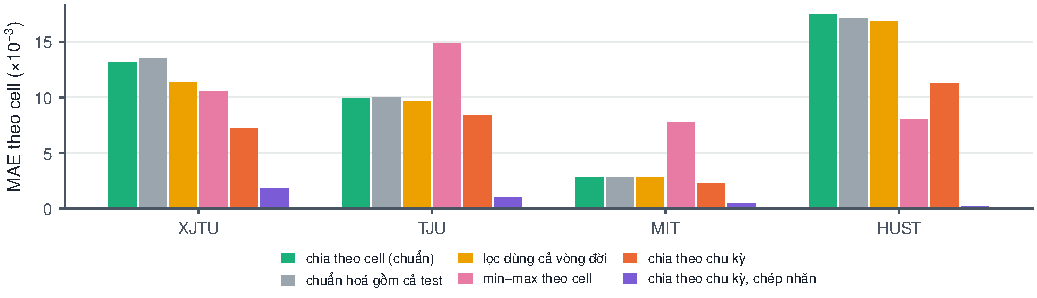
\includegraphics[width=\textwidth]{hinh/fig_thesis_leakage.pdf}
\caption[MAE theo cell của cùng một mô hình (MLP, 70\,\% nhãn) dưới các cách chia và chuẩn hoá khác nhau; vạch đứt là cách chia đúng (theo cell)]{MAE theo cell của cùng một mô hình (MLP, 70\,\% nhãn) dưới các cách chia và chuẩn hoá khác nhau; vạch đứt là cách chia đúng (theo cell). Điểm càng lệch trái so với vạch, sai số càng bị đánh giá thấp giả tạo.}\label{fig:leak}
\end{figure}


Hình~\ref{fig:leak} cho thấy mức độ nghiêm trọng của từng dạng rò rỉ. Chia theo chu kỳ làm sai số thấp đi
1{,}2--1{,}8 lần so với chia theo cell, dù mô hình và dữ liệu không đổi. Thiết lập cuối còn rõ hơn: một
bộ “dự đoán” không dùng đặc trưng nào, chỉ chép nhãn của chu kỳ train gần nhất trong cùng cell, đạt sai số
thấp hơn mọi mô hình thật được đánh giá đúng cách, đúng như Mệnh đề~\ref{md:rowleak} dự báo. Chuẩn hoá min--max theo vòng đời cell làm sai số thấp giả tạo trên XJTU và HUST (tỉ số XJTU 0{,}80, HUST 0{,}46), vì đầu vào đã chứa vị trí tương đối của chu kỳ trong vòng đời; ở hai bộ này SOH cuối đời của mọi cell gần như bằng nhau (XJTU 0{,}78--0{,}89, HUST 0{,}80--0{,}82; Bảng~\ref{tab:datastats}), nên biết vị trí trong vòng đời gần như đủ để suy ra SOH. Ngược lại, trên TJU và MIT cùng phép chuẩn hoá đó làm sai số tăng (tỉ số TJU 1{,}51, MIT 2{,}76): SOH cuối đời ở đây trải rộng hơn (TJU 0{,}66--0{,}90, MIT 0{,}82--0{,}97), nên vị trí trong vòng đời không đủ để suy ra SOH, trong khi chuẩn hoá theo từng cell lại xoá mất mức tuyệt đối của đặc trưng, vốn là thông tin phân biệt cell này với cell khác. Dù theo chiều nào, con số đo được cũng không phản ánh sai số khi triển khai, vì tuổi thọ của một cell đang vận hành chưa biết trước. Hai dạng còn lại tác động nhỏ hơn (lọc dùng cả vòng đời: 0{,}87--1{,}01; chuẩn hoá gồm cả test: 0{,}98--1{,}03), nhưng vẫn là rò rỉ và vẫn được loại bỏ trong giao thức chuẩn. Mọi
kết quả từ đây trở đi dùng giao thức chuẩn của Chương~\ref{ch:thietke}.

\section{PINN và học có nhãn khi thay đổi lượng nhãn}\label{sec:labels}

Bảng~\ref{tab:big} và Hình~\ref{fig:curvephys} là kết quả trung tâm của đồ án: sai số của
mọi mô hình ở bốn mức nhãn.

\begin{table}[!htbp]\centering\small
\caption[MAE theo cell của mọi mô hình theo lượng nhãn]{MAE theo cell (×$10^{-3}$) của mọi mô hình theo lượng nhãn (phần trăm số cell có nhãn); in đậm là thấp nhất trong cột của mỗi bộ. Trung bình 5 lần lặp × 5 fold; mỗi cell được test 5 lần.}\label{tab:big}
\begin{adjustbox}{max width=\textwidth}\begin{tabular}{llrrrr}\toprule
Bộ & Mô hình & 10\,\% & 30\,\% & 50\,\% & 70\,\% \\\midrule
XJTU & Ridge & 18{,}22 & 15{,}54 & 14{,}81 & 14{,}09 \\
 & GPR & 14{,}85 & 12{,}11 & 14{,}86 & 19{,}18 \\
 & GBDT & \textbf{14{,}49} & \textbf{10{,}85} & \textbf{10{,}19} & \textbf{9{,}51} \\
 & MLP & 24{,}72 & 15{,}95 & 14{,}58 & 12{,}74 \\
 & PINN-sup & 20{,}25 & 14{,}54 & 13{,}21 & 12{,}19 \\
 & PINN hộp đen & 15{,}68 & 14{,}15 & 12{,}82 & 12{,}34 \\
 & PINN-semi & 14{,}93 & 13{,}44 & 13{,}52 & 12{,}19 \\
\addlinespace[3pt]
TJU & Ridge & 23{,}01 & 21{,}60 & 20{,}50 & 20{,}74 \\
 & GPR & 13{,}50 & 9{,}22 & 8{,}01 & 8{,}17 \\
 & GBDT & \textbf{12{,}68} & \textbf{8{,}14} & \textbf{7{,}21} & \textbf{6{,}77} \\
 & MLP & 15{,}50 & 11{,}33 & 9{,}99 & 9{,}64 \\
 & PINN-sup & 14{,}73 & 10{,}67 & 10{,}20 & 10{,}52 \\
 & PINN hộp đen & 13{,}90 & 10{,}91 & 10{,}36 & 10{,}16 \\
 & PINN-semi & 13{,}91 & 10{,}85 & 10{,}46 & 10{,}52 \\
\addlinespace[3pt]
MIT & Ridge & 3{,}53 & 3{,}24 & 3{,}17 & 3{,}13 \\
 & GPR & 3{,}21 & 2{,}14 & 1{,}84 & 1{,}79 \\
 & GBDT & \textbf{3{,}09} & \textbf{1{,}99} & \textbf{1{,}73} & \textbf{1{,}58} \\
 & MLP & 8{,}54 & 3{,}40 & 3{,}04 & 2{,}86 \\
 & PINN-sup & 5{,}34 & 2{,}69 & 2{,}54 & 2{,}44 \\
 & PINN hộp đen & 4{,}19 & 2{,}80 & 2{,}61 & 2{,}54 \\
 & PINN-semi & 3{,}34 & 2{,}58 & 2{,}48 & 2{,}44 \\
\addlinespace[3pt]
HUST & Ridge & \textbf{22{,}88} & 18{,}85 & 18{,}32 & 18{,}10 \\
 & GPR & 28{,}82 & 21{,}24 & 18{,}50 & 17{,}22 \\
 & GBDT & 24{,}13 & 18{,}63 & \textbf{15{,}65} & \textbf{14{,}45} \\
 & MLP & 37{,}95 & 19{,}80 & 17{,}73 & 16{,}94 \\
 & PINN-sup & 31{,}67 & 17{,}82 & 16{,}11 & 15{,}99 \\
 & PINN hộp đen & 24{,}04 & 17{,}49 & 16{,}47 & 15{,}99 \\
 & PINN-semi & 22{,}98 & \textbf{17{,}30} & 16{,}11 & 15{,}99 \\
\bottomrule\end{tabular}\end{adjustbox}\end{table}

\begin{figure}[!htbp]\centering
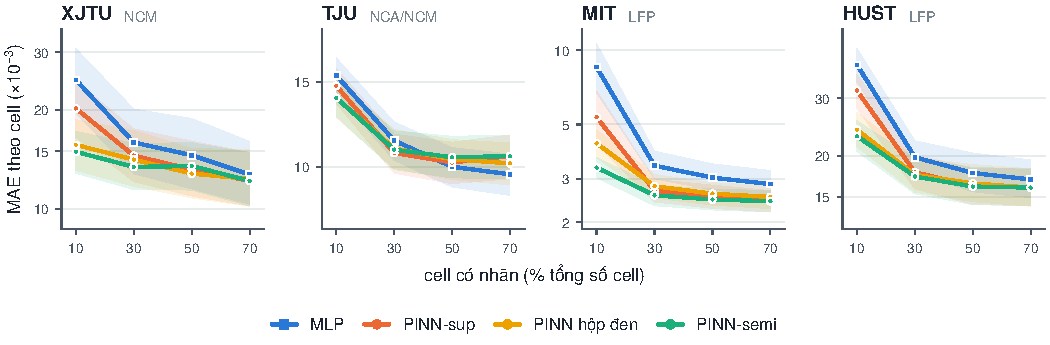
\includegraphics[width=\textwidth]{hinh/fig_thesis_curve_physics.pdf}
\caption[MAE theo cell theo lượng nhãn: MLP và các biến thể có vật lý]{MAE theo cell theo lượng nhãn: MLP và các biến thể có vật lý. Dải là khoảng tin cậy 95\,\% bootstrap theo cell; trục dọc thang log.}\label{fig:curvephys}
\end{figure}



\paragraph{Khi có ít nhãn.} Ở 10\,\% nhãn, PINN-semi vượt MLP với khoảng cách lớn nhất: tỉ số MAE
(Bảng~\ref{tab:cmp}) là XJTU 0{,}60, TJU 0{,}90, MIT 0{,}39, HUST 0{,}61,
có ý nghĩa trên cả bốn bộ. Ở mức này mỗi fold chỉ có 6--13 (XJTU 6, TJU 13, MIT 12, HUST 8) cell có nhãn, và MLP dễ quá khớp; loss vật lý trên các
cell không nhãn buộc mạng phải cho quỹ đạo hợp lý trên chính những cell nó chưa có nhãn, nên bù được phần lớn
thông tin thiếu.

\paragraph{Ở 30\,\% nhãn.} PINN-semi có MAE theo cell thấp hơn MLP có ý nghĩa thống kê (Wilcoxon theo cell,
hiệu chỉnh Holm) trên cả bốn bộ, với tỉ số MAE từ 0{,}76 (MIT) tới 0{,}96 (TJU). Với kiểm định bảo thủ ở mức fold, kết luận chỉ còn đứng vững trên MIT; XJTU, TJU và HUST có hướng cải thiện nhất quán nhưng biến thiên giữa các lần huấn luyện còn lớn so với mức cải thiện.

\paragraph{Khi có nhiều nhãn.} Ở 70\,\% nhãn, mọi cell train đều có nhãn và không còn cell không nhãn, nên
PINN-semi và PINN-sup trùng nhau; vật lý lúc này chỉ còn vai trò một bộ chuẩn hoá. Tỉ số MAE so với MLP là
XJTU 0{,}96, TJU 1{,}09, MIT 0{,}85, HUST 0{,}94; cải thiện có ý nghĩa trên MIT; trên TJU MLP lại tốt hơn có ý nghĩa. Trung bình nhân của tỉ số qua bốn bộ tiến dần về 1 khi lượng nhãn tăng:
10\,\%: 0{,}60, 30\,\%: 0{,}86, 50\,\%: 0{,}92, 70\,\%: 0{,}96. Dữ liệu có nhãn càng đủ, ràng buộc vật lý càng ít thông tin mới.

\paragraph{Lượng nhãn tương đương.} Bảng~\ref{tab:equiv} quy đổi kết quả sang số nhãn tiết kiệm được. Một giá trị
“$> 70\,\%$” nghĩa là mô hình học có nhãn chưa đạt được sai số đó ngay cả khi dùng toàn bộ nhãn train; “$\le
10\,\%$” nghĩa là mô hình học có nhãn đã đạt sai số đó ngay ở mức nhãn thấp nhất. So với MLP, PINN-semi dùng 10\,\% nhãn đạt sai số mà MLP cần XJTU 45\,\%, TJU 17\,\%, MIT 33\,\%, HUST 25\,\% nhãn mới đạt, tức tiết kiệm 1{,}7--4{,}5 lần số nhãn; PINN-semi dùng 30\,\% nhãn tương đương MLP dùng XJTU 62\,\%, TJU 37\,\%, MIT $> 70\,\%$, HUST 61\,\%. So với mô hình học có nhãn tốt nhất ở từng mức thì khác: trên cả bốn bộ, mô hình học có nhãn tốt nhất đã đạt sai số của PINN-semi ngay ở 10\,\% nhãn; ở 30\,\% nhãn, PINN-semi vẫn tiết kiệm nhãn trên HUST (tương đương 38\,\%), còn trên XJTU, TJU và MIT mô hình tốt nhất chỉ cần 15--18\,\% nhãn để bằng PINN-semi 30\,\%.

\begin{table}[!htbp]\centering\small
\caption[Lượng nhãn tương đương]{Lượng nhãn tương đương: mô hình học có nhãn cần bao nhiêu phần trăm cell có nhãn để đạt MAE của PINN-semi ở 10\,\% và 30\,\% nhãn (“tốt nhất”: mô hình học có nhãn tốt nhất ở từng mức, trong Ridge, GPR, GBDT, MLP). Nội suy log-tuyến tính giữa các mức đo.}\label{tab:equiv}
\begin{adjustbox}{max width=\textwidth}\begin{tabular}{lrrrr}\toprule
Bộ & PINN 10\,\% ≈ MLP & PINN 10\,\% ≈ tốt nhất & PINN 30\,\% ≈ MLP & PINN 30\,\% ≈ tốt nhất \\\midrule
XJTU & 45\,\% & $\le 10\,\%$ & 62\,\% & 15\,\% \\
TJU & 17\,\% & $\le 10\,\%$ & 37\,\% & 17\,\% \\
MIT & 33\,\% & $\le 10\,\%$ & $> 70\,\%$ & 18\,\% \\
HUST & 25\,\% & $\le 10\,\%$ & 61\,\% & 38\,\% \\
\bottomrule\end{tabular}\end{adjustbox}\end{table}



\begin{table}[!htbp]\centering\scriptsize
\caption[Tỉ số MAE của PINN-semi so với MLP và GBDT]{Tỉ số MAE theo cell của PINN-semi so với MLP và GBDT ở từng mức nhãn (nhỏ hơn 1: PINN-semi tốt hơn). $^{*}$: $p_\text{Holm} < 0{,}05$ theo cell; $^{\dagger}$: còn có ý nghĩa với kiểm định bảo thủ mức fold.}\label{tab:cmp}
\begin{adjustbox}{max width=\textwidth}\begin{tabular}{llrrrrrr}\toprule
Bộ & Nhãn & so với MLP: tỉ số [KTC] & cell tốt hơn & $p_\text{Holm}$ & so với GBDT: tỉ số [KTC] & cell tốt hơn & $p_\text{Holm}$ \\\midrule
XJTU & 10\,\% & 0{,}60 [0{,}54; 0{,}68]$^{*}$ & 91\,\% & $<10^{-4}$ & 1{,}03 [0{,}93; 1{,}15] & 47\,\% & 0{,}8210 \\
 & 30\,\% & 0{,}84 [0{,}76; 0{,}93]$^{*}$ & 65\,\% & 0{,}0047 & 1{,}24 [1{,}11; 1{,}42]$^{*}$ & 31\,\% & 0{,}0004 \\
 & 50\,\% & 0{,}93 [0{,}81; 1{,}06] & 45\,\% & 0{,}7502 & 1{,}33 [1{,}17; 1{,}53]$^{*}$ & 20\,\% & $<10^{-4}$ \\
 & 70\,\% & 0{,}96 [0{,}90; 1{,}02] & 53\,\% & 0{,}4712 & 1{,}28 [1{,}11; 1{,}54]$^{*}$ & 33\,\% & 0{,}0010 \\
TJU & 10\,\% & 0{,}90 [0{,}87; 0{,}93]$^{*}$ & 75\,\% & $<10^{-4}$ & 1{,}10 [1{,}02; 1{,}18]$^{*}$ & 38\,\% & 0{,}0340 \\
 & 30\,\% & 0{,}96 [0{,}93; 0{,}99]$^{*}$ & 68\,\% & 0{,}0041 & 1{,}33 [1{,}24; 1{,}44]$^{*}$ & 28\,\% & $<10^{-4}$ \\
 & 50\,\% & 1{,}05 [1{,}01; 1{,}09] & 43\,\% & 0{,}2363 & 1{,}45 [1{,}33; 1{,}58]$^{*}$$^{\dagger}$ & 22\,\% & $<10^{-4}$ \\
 & 70\,\% & 1{,}09 [1{,}04; 1{,}14]$^{*}$ & 41\,\% & 0{,}0086 & 1{,}55 [1{,}40; 1{,}72]$^{*}$$^{\dagger}$ & 20\,\% & $<10^{-4}$ \\
MIT & 10\,\% & 0{,}39 [0{,}32; 0{,}48]$^{*}$ & 90\,\% & $<10^{-4}$ & 1{,}08 [1{,}00; 1{,}16] & 45\,\% & 0{,}1991 \\
 & 30\,\% & 0{,}76 [0{,}69; 0{,}83]$^{*}$$^{\dagger}$ & 82\,\% & $<10^{-4}$ & 1{,}30 [1{,}21; 1{,}40]$^{*}$$^{\dagger}$ & 18\,\% & $<10^{-4}$ \\
 & 50\,\% & 0{,}81 [0{,}75; 0{,}88]$^{*}$ & 79\,\% & $<10^{-4}$ & 1{,}43 [1{,}34; 1{,}54]$^{*}$$^{\dagger}$ & 9\,\% & $<10^{-4}$ \\
 & 70\,\% & 0{,}85 [0{,}79; 0{,}92]$^{*}$ & 74\,\% & $<10^{-4}$ & 1{,}54 [1{,}44; 1{,}67]$^{*}$$^{\dagger}$ & 6\,\% & $<10^{-4}$ \\
HUST & 10\,\% & 0{,}61 [0{,}55; 0{,}67]$^{*}$ & 92\,\% & $<10^{-4}$ & 0{,}95 [0{,}89; 1{,}02] & 61\,\% & 0{,}0720 \\
 & 30\,\% & 0{,}87 [0{,}82; 0{,}92]$^{*}$ & 71\,\% & $<10^{-4}$ & 0{,}93 [0{,}86; 1{,}00]$^{*}$ & 69\,\% & 0{,}0042 \\
 & 50\,\% & 0{,}91 [0{,}87; 0{,}95]$^{*}$ & 68\,\% & 0{,}0008 & 1{,}03 [0{,}95; 1{,}12] & 56\,\% & 0{,}9939 \\
 & 70\,\% & 0{,}94 [0{,}90; 0{,}99] & 65\,\% & 0{,}0526 & 1{,}11 [1{,}01; 1{,}22] & 43\,\% & 0{,}0923 \\
\bottomrule\end{tabular}\end{adjustbox}\end{table}


\section{So với các mô hình học có nhãn khác}

Ridge, dù chỉ là mô hình tuyến tính, tốt hơn MLP ở 10\,\% nhãn trên XJTU, MIT và HUST: khi rất ít nhãn, mô hình đơn giản ít quá khớp hơn. Nhưng Ridge cải thiện chậm khi thêm nhãn: MAE ở 70\,\% bằng 0{,}77--0{,}90 lần MAE ở 10\,\%, so với 0{,}33--0{,}62 lần của MLP. GPR chỉ dùng được 1\,500 điểm huấn luyện do chi phí $O(n^3)$ theo số điểm, và kém GBDT trong 16/16 trường hợp (bộ × mức nhãn); dù vậy GPR vẫn có MAE thấp hơn PINN-semi trong 10/16 trường hợp, và thấp hơn ở cả bốn mức nhãn trên TJU và MIT. GBDT là đối thủ mạnh nhất: mô hình này tốt hơn PINN-semi có ý nghĩa thống kê ở 10\,\% (TJU); 30\,\% (XJTU, TJU và MIT); 50\,\% (XJTU, TJU và MIT); 70\,\% (XJTU, TJU và MIT); ngược lại PINN-semi tốt hơn GBDT có ý nghĩa ở 30\,\% (HUST). Ở 10\,\% nhãn, tỉ số MAE của PINN-semi so với GBDT là XJTU 1{,}03, TJU 1{,}10, MIT 1{,}08, HUST 0{,}95. Cây quyết định xử lý tốt các đặc trưng có phân phối lệch và
các chế độ thí nghiệm khác hẳn nhau mà không cần chuẩn hoá cẩn thận; đây là ưu thế quen thuộc của mô hình cây trên
dữ liệu dạng bảng. Phát biểu đúng mức vì vậy là: vật lý cải thiện rõ rệt \emph{mô hình mạng nơ-ron} khi ít nhãn và
đưa nó tới gần mô hình cây ở 10\,\% nhãn (tỉ số so với GBDT 0{,}95--1{,}10), nhưng chưa vượt được một mô hình cây
được tinh chỉnh tốt, cũng như hồi quy Gauss, trên phần lớn các bộ dữ liệu.


\section{So với các mô hình học sâu theo đề cương}\label{sec:dlres}

Bảng~\ref{tab:allmae}, \ref{tab:allr2} và~\ref{tab:allrm} đặt bốn mô hình học sâu của đề cương (MLP, CNN,
LSTM, Transformer) cạnh GBDT, PINN-semi, PINN-lai và mô hình cuối, trên cùng fold, cùng cell có nhãn và cùng ba lần lặp.

\paragraph{Bốn mô hình học sâu.} Nhìn được nhiều chu kỳ giúp rõ rệt. So với MLP, tỉ số MAE theo cell của CNN là 0{,}37--0{,}90, của LSTM là 0{,}36--0{,}90 và của Transformer là 0{,}43--0{,}93;
mô hình chuỗi thấp hơn MLP có ý nghĩa ở 42/48 phép so (bốn bộ $\times$ bốn mức nhãn $\times$ ba mô hình;
Wilcoxon theo cell, hiệu chỉnh Holm qua bốn bộ). Lợi ích lớn nhất ở 10\,\% nhãn
(tỉ số 0{,}36--0{,}90), nơi MLP chỉ dựa vào đặc trưng của một chu kỳ và dễ quá khớp vài cell có nhãn; từ 30\,\% nhãn tỉ số là
0{,}64--0{,}93. Cửa sổ nhiều chu kỳ cho mô hình thấy xu thế của đặc trưng sạc và làm trung bình nhiễu đo của từng chu kỳ,
giống phần đầu vào có lịch sử ở Mục~\ref{sec:histres} nhưng do mạng tự học. Trong ba mô hình chuỗi, LSTM có MAE thấp
nhất ở 8/16 trường hợp.

\paragraph{So với GBDT và các mô hình có vật lý.} Mô hình chuỗi tốt nhất của từng trường hợp có MAE thấp hơn GBDT ở
4/16 trường hợp (mọi mức nhãn trên HUST) và thấp hơn PINN-semi ở 14/16 (tỉ số 0{,}66--1{,}09). PINN-lai thấp hơn cả ba mô hình chuỗi
ở 47/48 phép so (tỉ số 0{,}57--1{,}00, có ý nghĩa ở 40), và mô hình cuối có MAE bằng 0{,}77--0{,}96 lần mô hình chuỗi
tốt nhất của từng trường hợp, thấp hơn có ý nghĩa ở 14/16. Như vậy, trên các bộ dữ liệu này, mô hình chuỗi
thuần dữ liệu thường tốt hơn một PINN-semi đơn lẻ nhưng chưa thay được việc kết hợp nhóm PINN với GBDT.

\paragraph{Độ dài cửa sổ.} Tỉ số MAE validation của $L = 48$ so với $L = 16$ (trung bình qua bốn bộ và hai mức nhãn) là CNN 1{,}000, LSTM 0{,}989, Transformer 1{,}005; theo quy tắc chốt trước, CNN và Transformer dùng $L = 16$; LSTM dùng $L = 48$. CNN cho đúng cùng kết quả ở hai độ dài: vùng nhìn của hai lớp tích chập chỉ 13 chu kỳ, nên phần cửa sổ xa hơn không tới được đầu ra. Với LSTM, cửa sổ dài có lợi nhất trên TJU (0{,}94) và bất lợi nhất trên HUST (1{,}01). Với Transformer, cửa sổ dài có lợi nhất trên HUST (0{,}93) và bất lợi nhất trên XJTU (1{,}13). Đổi độ dài cửa sổ làm sai số validation thay đổi tối đa 13\,\% theo bộ, nhỏ hơn nhiều so với khác biệt giữa các mô hình.

\paragraph{RMSE, MAPE và $R^2$.} Mô hình có MAE thấp nhất cũng có $R^2$ cao nhất ở 14/16 trường hợp. Ở 30\,\% nhãn, RMSE và MAPE (Bảng~\ref{tab:allrm}) cũng thấp nhất ở PINN-lai hoặc mô hình cuối và cao nhất ở MLP trên cả bốn bộ.
$R^2$ gộp mọi cell của bộ nên phụ
thuộc vào độ trải của SOH giữa các cell: MLP ở HUST 10\,\% có $R^2$ âm, tức dự đoán kém hơn cả hằng số bằng SOH trung bình của bộ. Vì vậy $R^2$ chỉ dùng để so các mô hình trong cùng một bộ, còn MAE theo
cell là chỉ số chính.

\begin{table}[!htbp]\centering\footnotesize
\caption[MAE theo cell của mọi mô hình chính]{MAE theo cell ($\times10^{-3}$) trên test của mọi mô hình chính, 3 lần lặp $\times$ 5 fold, cùng fold và cell có nhãn; in đậm là thấp nhất mỗi hàng. PINN-lai là bản tinh chỉnh trên validation; mô hình cuối là PINN-lai dùng hay không dùng lịch sử theo validation (Mục~\ref{sec:histres}).}\label{tab:allmae}
\begin{adjustbox}{max width=\textwidth}\begin{tabular}{llrrrrrrrr}\toprule
Bộ & Nhãn & MLP & CNN & LSTM & Transformer & GBDT & PINN-semi & PINN-lai & Mô hình cuối \\\midrule
XJTU & 10\,\% & 23{,}27 & 16{,}01 & 16{,}62 & 17{,}63 & 14{,}01 & 14{,}65 & \textbf{12{,}71} & \textbf{12{,}71} \\
 & 30\,\% & 15{,}61 & 12{,}68 & 13{,}98 & 13{,}71 & 10{,}87 & 13{,}35 & \textbf{10{,}78} & \textbf{10{,}78} \\
 & 50\,\% & 14{,}10 & 11{,}69 & 11{,}98 & 12{,}05 & 10{,}18 & 13{,}20 & \textbf{10{,}02} & \textbf{10{,}02} \\
 & 70\,\% & 12{,}48 & 10{,}98 & 10{,}50 & 10{,}99 & 9{,}64 & 12{,}53 & \textbf{9{,}50} & \textbf{9{,}50} \\
TJU & 10\,\% & 15{,}81 & 14{,}22 & 13{,}08 & 14{,}14 & 12{,}60 & 14{,}01 & \textbf{11{,}70} & \textbf{11{,}70} \\
 & 30\,\% & 11{,}71 & 8{,}89 & 8{,}69 & 9{,}89 & 8{,}06 & 11{,}39 & 8{,}00 & \textbf{7{,}78} \\
 & 50\,\% & 9{,}96 & 7{,}31 & 7{,}24 & 9{,}31 & 7{,}17 & 10{,}74 & 7{,}23 & \textbf{6{,}92} \\
 & 70\,\% & 9{,}71 & 7{,}36 & 7{,}09 & 8{,}96 & 6{,}96 & 10{,}80 & 7{,}11 & \textbf{6{,}82} \\
MIT & 10\,\% & 9{,}02 & 3{,}30 & 3{,}26 & 3{,}87 & 3{,}15 & 3{,}29 & \textbf{2{,}52} & \textbf{2{,}52} \\
 & 30\,\% & 3{,}39 & 2{,}18 & 2{,}18 & 2{,}77 & 1{,}97 & 2{,}50 & \textbf{1{,}75} & \textbf{1{,}75} \\
 & 50\,\% & 3{,}06 & 1{,}99 & 2{,}04 & 2{,}71 & 1{,}74 & 2{,}45 & \textbf{1{,}59} & \textbf{1{,}59} \\
 & 70\,\% & 2{,}85 & 1{,}93 & 1{,}99 & 2{,}59 & 1{,}59 & 2{,}38 & \textbf{1{,}48} & \textbf{1{,}48} \\
HUST & 10\,\% & 41{,}62 & 22{,}77 & 24{,}51 & 21{,}95 & 23{,}84 & 22{,}76 & \textbf{20{,}36} & \textbf{20{,}36} \\
 & 30\,\% & 20{,}00 & 17{,}42 & 17{,}14 & 17{,}45 & 18{,}73 & 17{,}10 & 15{,}99 & \textbf{15{,}34} \\
 & 50\,\% & 18{,}13 & 15{,}04 & 15{,}52 & 16{,}00 & 15{,}82 & 16{,}42 & 14{,}26 & \textbf{13{,}17} \\
 & 70\,\% & 17{,}19 & 14{,}19 & 14{,}76 & 14{,}93 & 14{,}60 & 16{,}38 & 13{,}76 & \textbf{12{,}24} \\
\bottomrule\end{tabular}\end{adjustbox}\end{table}

\begin{table}[!htbp]\centering\footnotesize
\caption[$R^2$ của mọi mô hình chính]{$R^2$ trên test, tính trên dự đoán ghép 5 fold của một lần lặp (mỗi cell đúng một lần), bỏ 10 chu kỳ đầu mỗi cell, trung bình 3 lần lặp; in đậm là cao nhất mỗi hàng.}\label{tab:allr2}
\begin{adjustbox}{max width=\textwidth}\begin{tabular}{llrrrrrrrr}\toprule
Bộ & Nhãn & MLP & CNN & LSTM & Transformer & GBDT & PINN-semi & PINN-lai & Mô hình cuối \\\midrule
XJTU & 10\,\% & 0{,}434 & 0{,}743 & 0{,}745 & 0{,}736 & 0{,}793 & 0{,}813 & \textbf{0{,}830} & \textbf{0{,}830} \\
 & 30\,\% & 0{,}796 & 0{,}843 & 0{,}831 & 0{,}836 & 0{,}861 & 0{,}860 & \textbf{0{,}875} & \textbf{0{,}875} \\
 & 50\,\% & 0{,}825 & 0{,}859 & 0{,}866 & 0{,}867 & 0{,}879 & 0{,}856 & \textbf{0{,}888} & \textbf{0{,}888} \\
 & 70\,\% & 0{,}858 & 0{,}883 & \textbf{0{,}894} & 0{,}889 & 0{,}879 & 0{,}873 & 0{,}890 & 0{,}890 \\
TJU & 10\,\% & 0{,}903 & 0{,}923 & 0{,}929 & 0{,}925 & 0{,}926 & 0{,}931 & \textbf{0{,}941} & \textbf{0{,}941} \\
 & 30\,\% & 0{,}954 & 0{,}968 & 0{,}971 & 0{,}965 & 0{,}970 & 0{,}957 & 0{,}973 & \textbf{0{,}974} \\
 & 50\,\% & 0{,}965 & 0{,}977 & 0{,}978 & 0{,}968 & 0{,}976 & 0{,}961 & 0{,}978 & \textbf{0{,}979} \\
 & 70\,\% & 0{,}968 & 0{,}977 & 0{,}979 & 0{,}970 & 0{,}978 & 0{,}963 & 0{,}980 & \textbf{0{,}980} \\
MIT & 10\,\% & 0{,}679 & 0{,}980 & 0{,}971 & 0{,}970 & 0{,}973 & 0{,}974 & \textbf{0{,}987} & \textbf{0{,}987} \\
 & 30\,\% & 0{,}950 & 0{,}989 & 0{,}988 & 0{,}984 & 0{,}985 & 0{,}986 & \textbf{0{,}991} & \textbf{0{,}991} \\
 & 50\,\% & 0{,}964 & 0{,}991 & 0{,}991 & 0{,}987 & 0{,}990 & 0{,}986 & \textbf{0{,}993} & \textbf{0{,}993} \\
 & 70\,\% & 0{,}975 & 0{,}992 & 0{,}992 & 0{,}988 & 0{,}992 & 0{,}988 & \textbf{0{,}994} & \textbf{0{,}994} \\
HUST & 10\,\% & −0{,}083 & 0{,}802 & 0{,}749 & \textbf{0{,}836} & 0{,}783 & 0{,}770 & 0{,}827 & 0{,}827 \\
 & 30\,\% & 0{,}864 & 0{,}873 & 0{,}888 & 0{,}886 & 0{,}858 & 0{,}893 & 0{,}901 & \textbf{0{,}907} \\
 & 50\,\% & 0{,}878 & 0{,}909 & 0{,}907 & 0{,}910 & 0{,}896 & 0{,}902 & 0{,}917 & \textbf{0{,}931} \\
 & 70\,\% & 0{,}893 & 0{,}916 & 0{,}910 & 0{,}919 & 0{,}909 & 0{,}903 & 0{,}923 & \textbf{0{,}939} \\
\bottomrule\end{tabular}\end{adjustbox}\end{table}

\begin{table}[!htbp]\centering\footnotesize
\caption[RMSE và MAPE của mọi mô hình chính ở 30\,\% nhãn]{Ở 30\,\% nhãn: RMSE theo cell ($\times10^{-3}$) và MAPE (\%, gộp mọi chu kỳ) trên test; in đậm là thấp nhất mỗi cột.}\label{tab:allrm}
\begin{adjustbox}{max width=\textwidth}\begin{tabular}{lrrrrrrrr}\toprule
Mô hình & XJTU RMSE & MAPE & TJU RMSE & MAPE & MIT RMSE & MAPE & HUST RMSE & MAPE \\\midrule
MLP & 23{,}10 & 1{,}47 & 13{,}94 & 1{,}20 & 4{,}65 & 0{,}41 & 26{,}07 & 2{,}12 \\
CNN & 16{,}11 & 1{,}27 & 10{,}60 & 0{,}94 & 3{,}04 & 0{,}23 & 24{,}04 & 1{,}89 \\
LSTM & 17{,}91 & 1{,}32 & 10{,}27 & 0{,}94 & 3{,}05 & 0{,}23 & 23{,}45 & 1{,}85 \\
Transformer & 17{,}39 & 1{,}37 & 11{,}72 & 1{,}04 & 3{,}72 & 0{,}29 & 23{,}17 & 1{,}87 \\
GBDT & \textbf{14{,}37} & 1{,}19 & 9{,}74 & 0{,}90 & 2{,}93 & 0{,}21 & 25{,}98 & 2{,}04 \\
PINN-semi & 19{,}42 & 1{,}32 & 13{,}54 & 1{,}16 & 3{,}34 & 0{,}28 & 22{,}84 & 1{,}83 \\
PINN-lai & 14{,}37 & \textbf{1{,}16} & 9{,}54 & 0{,}87 & \textbf{2{,}47} & \textbf{0{,}18} & \textbf{21{,}86} & 1{,}72 \\
Mô hình cuối & 14{,}37 & 1{,}16 & \textbf{9{,}22} & \textbf{0{,}85} & 2{,}47 & 0{,}18 & 22{,}38 & \textbf{1{,}65} \\
\bottomrule\end{tabular}\end{adjustbox}\end{table}

\section{Lợi ích đến từ đâu}\label{sec:source}

Bảng~\ref{tab:source} tách mức giảm sai số của PINN-semi so với MLP ở 30\,\% nhãn theo từng thành phần.

\begin{table}[!htbp]\centering\small
\caption[Tách nguồn gốc lợi ích ở 30\,\% nhãn]{Tách nguồn gốc lợi ích ở 30\,\% nhãn: MAE theo cell (×$10^{-3}$), trong ngoặc là tỉ số so với MLP.}\label{tab:source}
\begin{adjustbox}{max width=\textwidth}\begin{tabular}{lrrrr}\toprule
Mô hình (30\,\% nhãn) & XJTU & TJU & MIT & HUST \\\midrule
MLP & 15{,}95 & 11{,}33 & 3{,}40 & 19{,}80 \\
PINN-sup & 14{,}54 (0{,}91) & 10{,}67 (0{,}94) & 2{,}69 (0{,}79) & 17{,}82 (0{,}90) \\
chỉ đơn điệu & 14{,}13 (0{,}89) & 11{,}00 (0{,}97) & 2{,}86 (0{,}84) & 17{,}41 (0{,}88) \\
PINN-semi (Euler) & 13{,}37 (0{,}84) & 11{,}31 (1{,}00) & 3{,}01 (0{,}89) & 17{,}49 (0{,}88) \\
PINN hộp đen & 14{,}15 (0{,}89) & 10{,}91 (0{,}96) & 2{,}80 (0{,}83) & 17{,}49 (0{,}88) \\
PINN-semi & 13{,}44 (0{,}84) & 10{,}85 (0{,}96) & 2{,}58 (0{,}76) & 17{,}30 (0{,}87) \\
\bottomrule\end{tabular}\end{adjustbox}\end{table}


\begin{itemize}
\item \emph{Vật lý chỉ trên cell có nhãn} (PINN-sup): ở 10\,\% nhãn tỉ số so với MLP là XJTU 0{,}82, TJU 0{,}95, MIT 0{,}63, HUST 0{,}83. Vật lý đóng vai trò bộ chuẩn hoá có giúp, nhưng còn xa mới bằng PINN-semi.
\item \emph{Thêm cell không nhãn} (PINN-semi so với PINN-sup): tỉ số XJTU 0{,}74, TJU 0{,}94, MIT 0{,}62, HUST 0{,}73 ở 10\,\% và XJTU 0{,}92, TJU 1{,}02, MIT 0{,}96, HUST 0{,}97 ở 30\,\% nhãn. Tính theo thang log, phần này chiếm 50--64\,\% mức giảm sai số của PINN-semi so với MLP ở 10\,\% nhãn, phần còn lại đến từ vật lý trên cell có nhãn. Ở mức nhãn thấp, dữ liệu không nhãn đóng góp ít nhất ngang với vật lý trên cell có nhãn, và nó chỉ có ích khi được nối với mô hình qua loss vật lý không dùng nhãn.
\item \emph{Phương trình động học so với chỉ đơn điệu}: chỉ với ràng buộc đơn điệu, mô hình đã đạt 62--95\,\% mức giảm sai số (thang log) của PINN-semi so với MLP ở 30\,\% nhãn. Khi bỏ $\mathcal{L}_\text{ode}$ và $\mathcal{L}_\text{range}$, MAE bằng XJTU 1{,}05, TJU 1{,}01, MIT 1{,}11, HUST 1{,}01 lần PINN-semi đầy đủ, chênh lệch lớn nhất ở MIT: phần còn lại của lợi ích đến từ cấu trúc động học.
\item \emph{Dạng phần dư}: MAE của phần dư Euler dọc quỹ đạo so với dạng đạo hàm riêng theo $t$ là XJTU 0{,}99, TJU 1{,}04, MIT 1{,}17, HUST 1{,}01: ngang nhau trên XJTU và HUST; kém hơn trên TJU và MIT.
\item \emph{Động học hộp đen} (kiểu PINN4SOH) so với động học xám: tỉ số MAE của PINN hộp đen so với PINN-semi là XJTU 1{,}05, TJU 1{,}00, MIT 1{,}26, HUST 1{,}05 ở 10\,\% và XJTU 1{,}05, TJU 1{,}01, MIT 1{,}09, HUST 1{,}01 ở 30\,\% nhãn. Theo kiểm định Wilcoxon có hiệu chỉnh Holm, động học xám tốt hơn có ý nghĩa ở 10\,\% (MIT và HUST); 30\,\% (MIT); 50\,\% (HUST), hộp đen tốt hơn có ý nghĩa ở 50\,\% (XJTU); 11 trường hợp còn lại (trong 16 cặp bộ × mức nhãn) khác biệt không có ý nghĩa. Khác biệt lớn nhất ở MIT với 10\,\% nhãn, khi MAE của PINN hộp đen bằng 1{,}26 lần PINN-semi. Ở 30\,\% nhãn, sai số của PINN hộp đen gần như trùng với biến thể chỉ đơn điệu (chênh không quá 2\,\%). Điều này phù hợp với giả thuyết: khi $G$ nhận cả $u_t$ làm đầu vào, mạng có thể học $G \approx u_t$ nên phần dư động học bị thoả mãn tầm thường, chỉ còn ràng buộc đơn điệu và miền giá trị có tác dụng; động học xám không có lối thoát này vì $r$ không phụ thuộc $u_t$ và luôn không âm.
\end{itemize}

\section{Quỹ đạo dự đoán theo lượng nhãn}






Hình~\ref{fig:traj} đặt cạnh nhau dự đoán cho cùng một cell khi lượng nhãn tăng từ 10 lên 30 và 70\,\%. Khi ít nhãn,
cả hai mô hình bám được hình dạng của quỹ đạo nhưng lệch mức, rõ nhất ở TJU và HUST; thêm nhãn chủ yếu làm giảm phần
lệch mức này chứ không làm thay đổi hình dạng. Ở 10\,\% nhãn, dự đoán của MLP dao động mạnh hơn và có những đoạn đi
lên, còn PINN-semi giữ được xu hướng giảm; khoảng cách giữa hai mô hình thu hẹp dần khi nhãn tăng.

\begin{figure}[!htbp]\centering
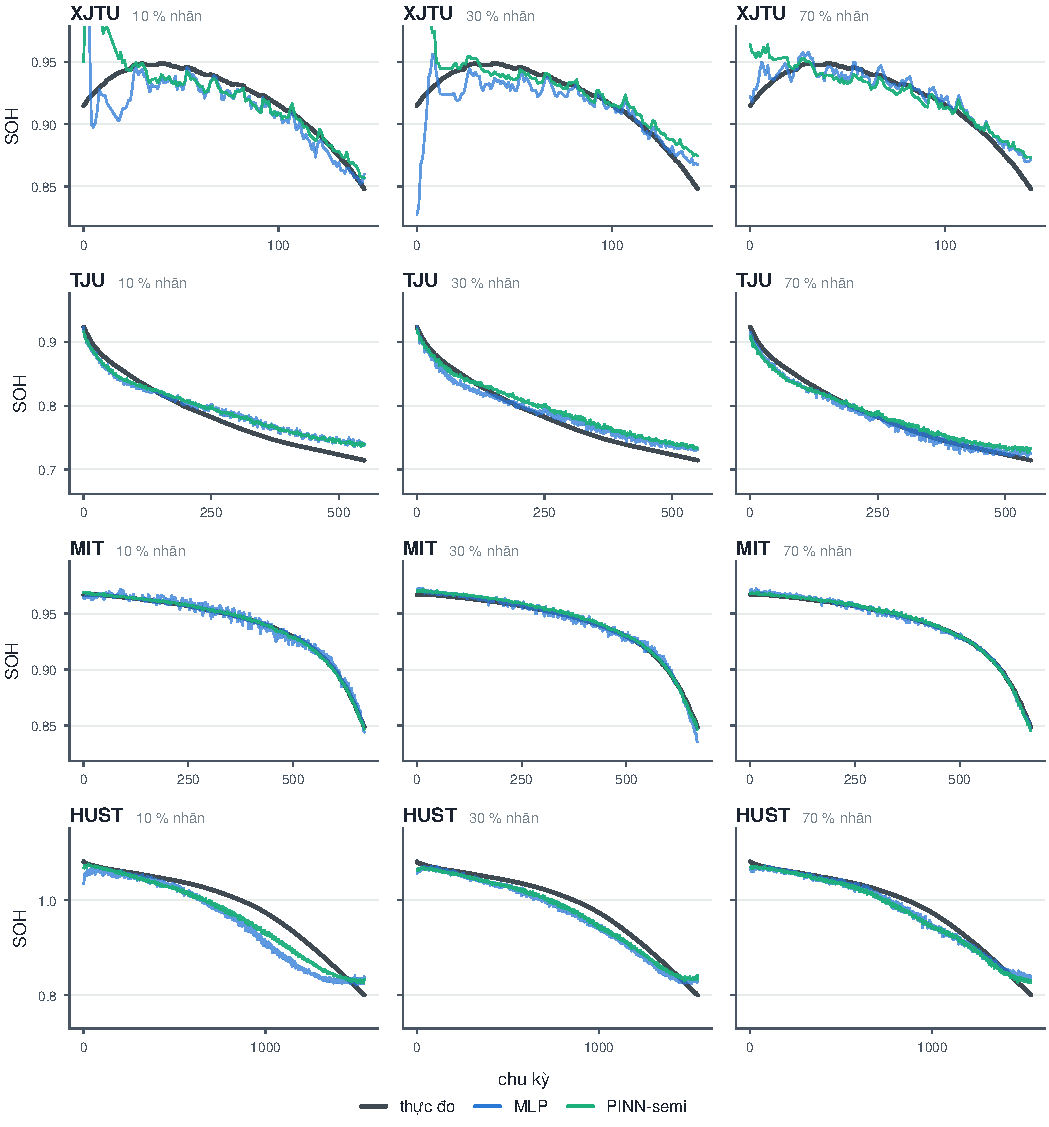
\includegraphics[width=0.92\textwidth]{hinh/fig_pred_traj.pdf}
\caption[Quỹ đạo SOH của cùng một cell test mỗi bộ khi có 10, 30 và 70\,\% số cell mang nhãn (lần lặp 0)]{Quỹ đạo SOH của cùng một cell test mỗi bộ khi có 10, 30 và 70\,\% số cell mang nhãn (lần lặp 0). Cell được chọn là cell có sai số MLP ở trung vị của bộ tại 30\,\% nhãn, bỏ qua các cell có nhãn nhảy bất thường giữa hai chu kỳ; trục dọc theo dải SOH thực đo nên vài chu kỳ đầu của XJTU vượt khỏi khung.}\label{fig:traj}
\end{figure}



\section{Tham số vật lý học được}\label{sec:physparams}



Cả hai tham số vật lý gần như không rời giá trị khởi tạo: $\lambda$ nằm trong khoảng 0{,}96--0{,}97 trên mọi bộ (khởi tạo 1), $E_a$ dịch XJTU 0{,}0, TJU 1{,}1, MIT 1{,}0, HUST 1{,}1\,kJ/mol. Trên XJTU, nhiệt độ thí nghiệm trùng $T_\text{ref} = 25$\,\textdegree C nên $A(T) = 1$ và gradient theo $E_a$ bằng 0; trên MIT và HUST, mọi cell cùng 30\,\textdegree C nên $A(T)$ chỉ là một hằng số nhân, không tách được khỏi $k(\mathbf{x})$. Ngay cả trên TJU, nơi có ba mức nhiệt độ, $E_a$ cũng chỉ dịch chừng 1\,kJ/mol: với trọng số $\alpha = 0{,}02$, tín hiệu từ $\mathcal{L}_\text{ode}$ quá yếu để ước lượng $E_a$, và mạng $k(\mathbf{x})$ có thể tự hấp thụ ảnh hưởng của nhiệt độ qua đặc trưng sạc. Vì vậy hai tham số này nên được hiểu là phần cấu trúc của ràng buộc (dấu và dạng hàm của tốc độ suy giảm), không phải đại lượng vật lý được ước lượng từ dữ liệu.


Hai giải thích trên được tách bằng một thí nghiệm bổ sung trên NASA (4, 24, 43\,\textdegree C) và TJU (25, 35,
45\,\textdegree C): huấn luyện lại PINN-semi ở 70\,\% nhãn với $\alpha$ tăng lên 0{,}2 và 1, có hoặc không thêm ràng buộc
Euler, và với khởi tạo $\lambda = 3$, $E_a = 60$\,kJ/mol. Hiệu giữa giá trị học được của hai cách khởi tạo bằng 1{,}00--1{,}01 lần
hiệu khởi tạo với $\lambda$ và 0{,}99--1{,}01 lần với $E_a$, kể cả khi ràng buộc ODE mạnh gấp 50 lần: tham số đứng yên ở nơi được
đặt. Giải thích hợp lý nhất nằm ở cấu trúc: tốc độ suy giảm chỉ xuất hiện dưới dạng tích $k(\mathbf{x})\,g(u)\,A(T)$, mà
$k(\mathbf{x})$ nhận chính các đặc trưng sạc vốn đã mang thông tin về nhiệt độ và mức SOH, nên $k$ bù lại mọi thay đổi
của $\lambda$ hay $E_a$. Sai số của các nhánh không khác cấu hình chuẩn có ý nghĩa (tỉ số MAE 0{,}93--1{,}12); thêm ràng buộc Euler cho tỉ số 0{,}93 trên NASA và 1{,}25 trên TJU (có ý nghĩa).
\section{Kiểm tra phần vật lý}\label{sec:physcheck}

Mục~\ref{sec:wherephys} chỉ ra rằng ba hàm mất mát vật lý tác động vào hai hướng khác nhau của hàm $F_\varphi$:
$\mathcal{L}_\text{mono}$ tác động lên tổng biến thiên dọc quỹ đạo thật của cell, $\mathcal{L}_\text{ode}$ tác động
lên đạo hàm riêng theo thời gian khi giữ nguyên đặc trưng sạc. Mục này đo riêng từng hướng trên các cell test.

\paragraph{Dọc quỹ đạo: tính đơn điệu của dự đoán.} Với mỗi cell test, đếm các cặp chu kỳ cách nhau ít nhất 10 chu
kỳ mà SOH dự đoán ở chu kỳ sau cao hơn chu kỳ trước quá 0,002, tức đúng ngưỡng của $\mathcal{L}_\text{mono}$. Phép
đếm này không cần nhãn, nên làm được với mọi mô hình; làm trên chính nhãn thật cho mức tham chiếu, vì dung lượng
thật có thể hồi phục nhẹ sau thời gian nghỉ. Ở 30\,\% nhãn, dự đoán của
MLP tăng ngược ở 13{,}6--31{,}1\,\% số cặp, của PINN-semi chỉ 3{,}0--12{,}0\,\%, trong khi nhãn thật là 0{,}1--7{,}7\,\%.
Biến thể chỉ đơn điệu cho tỉ lệ gần như bằng PINN-semi (3{,}1--12{,}4\,\%): chính $\mathcal{L}_\text{mono}$, áp lên cặp chu kỳ của cả cell không nhãn, làm quỹ đạo dự đoán đơn điệu.




\paragraph{Theo thời gian: đạo hàm riêng và phần dư ODE.} Đại lượng mà $\mathcal{L}_\text{ode}$ ràng buộc là
$\partial F_\varphi/\partial t$, chỉ tính được từ chính mô hình. Trọng số mô hình không được lưu, nhưng huấn luyện
là tất định, nên đồ án huấn luyện lại các lượt của MLP, PINN-semi, các biến thể cắt bỏ và PINN hộp đen ở 30\,\% nhãn,
lần lặp đầu, cả 5 fold trên 4 bộ: 120/120 lượt cho MAE trùng từng bit với lượt đã báo cáo. Trên cell test của
từng lượt, đo $\partial F_\varphi/\partial t$ bằng vi phân tự động, tốc độ $r$ của động học xám, và tách tổng mức
giảm SOH dự đoán trên vòng đời cell thành phần do biến thời gian
$\sum_i [F_\varphi(\tilde{\mathbf{x}}_i, t_{i+1}) - F_\varphi(\tilde{\mathbf{x}}_i, t_i)]$ và phần do đặc trưng sạc
$\sum_i [F_\varphi(\tilde{\mathbf{x}}_{i+1}, t_{i+1}) - F_\varphi(\tilde{\mathbf{x}}_i, t_{i+1})]$; hai phần cộng lại
đúng bằng tổng (Bảng~\ref{tab:physcheck}).

\begin{table}[!htbp]\centering\footnotesize
\caption[Kiểm tra phần vật lý trên cell test]{Đo trên cell test của mô hình đã huấn luyện (30\,\% nhãn, lần lặp đầu, 5 fold). Bốn cột đầu: tỉ lệ điểm có $\partial F_\varphi/\partial t > 0$ (\%). Ba cột giữa: trung vị qua các cell của phần giảm SOH dự đoán do riêng biến thời gian (\%). Ba cột cuối: tốc độ suy giảm trung bình (SOH trên 1\,000 chu kỳ).}\label{tab:physcheck}
\begin{adjustbox}{max width=\textwidth}\begin{tabular}{lrrrrrrrrrr}\toprule
 & \multicolumn{4}{c}{$\partial F_\varphi/\partial t > 0$ (\%)} & \multicolumn{3}{c}{phần do thời gian (\%)} & \multicolumn{3}{c}{tốc độ suy giảm} \\ \cmidrule(lr){2-5}\cmidrule(lr){6-8}\cmidrule(lr){9-11}
Bộ & MLP & chỉ đ.điệu & PINN-semi & Euler & MLP & PINN-semi & Euler & $r$ PINN-semi & $r$ Euler & thực đo \\\midrule
XJTU & 11{,}8 & 0{,}1 & 0{,}8 & 0{,}0 & 15 & 18 & 27 & 0{,}061 & 0{,}348 & 0{,}300 \\
TJU & 32{,}6 & 13{,}4 & 2{,}6 & 25{,}1 & 9 & 15 & 19 & 0{,}058 & 0{,}331 & 0{,}356 \\
MIT & 30{,}3 & 14{,}3 & 23{,}9 & 12{,}8 & 3 & 2 & 7 & 0{,}001 & 0{,}213 & 0{,}137 \\
HUST & 17{,}4 & 6{,}3 & 4{,}8 & 6{,}2 & 36 & 49 & 48 & 0{,}063 & 0{,}128 & 0{,}137 \\
\bottomrule\end{tabular}\end{adjustbox}\end{table}


Ba nhận xét. Thứ nhất, MLP có $\partial F_\varphi/\partial t > 0$, tức SOH tăng theo thời gian khi đặc trưng giữ
nguyên, ở 12--33\,\% số điểm test; PINN-semi giảm tỉ lệ này xuống 1--24\,\%, giảm rõ trên XJTU, TJU và HUST. Riêng MIT, ràng buộc được thoả theo cách tầm thường: $r$ học được gần bằng 0 (MIT 0{,}001) và đạo hàm theo thời gian cũng gần bằng 0, nên dấu của đạo hàm chỉ còn là nhiễu quanh 0. Thứ hai, ở mọi
mô hình, phần lớn mức giảm SOH dự đoán đi qua đặc trưng sạc chứ không qua biến thời gian: phần do thời gian chỉ
chiếm 3--36\,\% với MLP và 2--49\,\% với PINN-semi; với PINN-semi, phần này dưới 25\,\% trên XJTU, TJU và MIT và cao
nhất trên HUST (49\,\%). Mạng nghiệm nhận ra pin đã già chủ yếu nhờ đường sạc đã đổi dạng, và $\mathcal{L}_\text{ode}$ chỉ
ràng buộc phần còn lại. Thứ ba, phần dư ODE nhỏ so với chính đạo hàm
($|\partial_t F_\varphi + r|$ bằng XJTU 14, TJU 16, HUST 22\,\% của $|\partial_t F_\varphi|$), nghĩa là ràng buộc được thoả trên cell chưa từng thấy.

\paragraph{Tốc độ suy giảm học được.} Đồ án so tốc độ suy giảm thực đo của từng cell test (độ
dốc của SOH theo chu kỳ) với tốc độ của mô hình. Độ dốc của SOH dự đoán bám sát thực đo ở cả MLP lẫn PINN-semi
(tương quan hạng Spearman 0{,}30--0{,}99 với MLP, 0{,}31--0{,}99 với PINN-semi); trên HUST tương quan thấp hơn vì tốc độ của các cell gần như nhau (hệ số biến thiên 0{,}19, so với 0{,}39--1{,}66 ở các bộ khác). Tốc độ $r$ của
PINN-semi thì không: trung bình chỉ 0{,}001--0{,}063 so với 0{,}137--0{,}356 thực đo, và gần như không tương quan với tốc độ của từng
cell (Spearman XJTU −0{,}26, TJU 0{,}10, MIT −0{,}14, HUST 0{,}09). Lý do nằm ở nhận xét thứ hai: ở dạng đạo hàm riêng, $r$ được khớp với
$-\partial F_\varphi/\partial t$, tức chỉ với phần suy giảm mà mạng gán cho biến thời gian. Dạng Euler khớp $r$ với
tổng biến thiên dọc quỹ đạo, nên $r$ của nó xấp xỉ tốc độ thật (trung bình 0{,}128--0{,}348) và tương quan với tốc độ từng cell
(Spearman XJTU 0{,}72, TJU 0{,}88, MIT 0{,}66, HUST −0{,}22), rõ trên XJTU, TJU và MIT. Đổi lại, dạng Euler có MAE cao hơn dạng đạo hàm riêng trên TJU và MIT (Mục~\ref{sec:source}).



Đồ án xếp tốc độ suy giảm theo khoảng SOH thực đo. Trên XJTU, MIT và HUST, tốc độ thực đo ở khoảng SOH thấp nhất cao gấp 2--175 lần ở khoảng SOH cao nhất: đây là hiện tượng đầu gối. Trên TJU, đường trung bình không đi lên đều theo SOH. Giữa các khoảng SOH, $r$ chỉ thay đổi
1{,}4--1{,}9 lần (bỏ qua MIT, nơi $r \approx 0$) trong khi tốc độ thực đo thay đổi 3--175 lần, và với $\lambda \approx 0{,}96$ thừa số
$g(u) = e^{\lambda(1-u)}$ chỉ tăng khoảng 1,2 lần khi SOH giảm từ 1 xuống 0,8: đầu gối trong dự đoán đến từ đặc trưng
sạc, không đến từ thừa số đầu gối của động học.



Tóm lại, phần vật lý giúp mô hình chủ yếu qua ràng buộc dọc quỹ đạo: dự đoán của PINN-semi gần đơn điệu như nhãn
thật, và đây cũng là phần mang lại phần lớn lợi ích về sai số (Mục~\ref{sec:source}). Ràng buộc ODE dạng đạo hàm riêng
giữ cho SOH không tăng theo thời gian, nhưng tốc độ $r$ của nó không phải là ước lượng tốc độ suy giảm của cell; muốn
$r$ diễn giải được theo nghĩa vật lý cần dạng Euler.


\section{Mô hình kết hợp PINN-lai}\label{sec:improve}
\subsection{Sai số còn lại nằm ở đâu}\label{sec:errdecomp}

Trước khi thử cải tiến, cần biết sai số hiện tại có dạng gì. Với mỗi cell test, sai số theo chu kỳ
$e_n = \hat y_n - y_n$ được tách thành ba phần:
\begin{equation}
e_n = \underbrace{b}_{\text{lệch mức}} + \underbrace{s_n}_{\text{trôi chậm}} + \underbrace{f_n}_{\text{dao động nhanh}},
\end{equation}
trong đó $b$ là trung bình của $e_n$ trên cả cell, $s_n$ là trung bình trượt căn giữa 21 điểm của $e_n - b$, còn $f_n$
là phần còn lại. Ở 30\,\% nhãn, với MLP, PINN-semi và GBDT trên bốn bộ, lệch mức chiếm 14--58\,\% tổng MSE và trôi chậm
32--57\,\%. Phần dao động nhanh, tức nhiễu giữa các chu kỳ liền nhau, chỉ chiếm 1--17\,\% tổng MSE ngoài bộ MIT; trên MIT, nơi
sai số tuyệt đối rất nhỏ, phần này lên tới 25--34\,\%. Phần lớn sai số là lệch mức và trôi chậm: mô hình đoán sai
SOH của cả một cell, hoặc đoán sai tốc độ suy giảm trên một đoạn dài. Hai hệ quả rút ra. Một là làm trơn dự đoán chỉ
giúp được một phần nhỏ. Hai là muốn giảm sai số đáng kể phải giảm phần lệch theo từng cell, và cách đơn giản nhất là
lấy trung bình những mô hình có lệch theo cell khác nhau.

\subsection{Chọn hướng trên tập validation}\label{sec:devproto}

Giai đoạn phát triển dùng lần lặp 0, cả 5 fold, hai mức nhãn 10\,\% và 50\,\%. Mỗi fold có khoảng 10\,\% số cell
làm validation, tách khỏi cả train lẫn test; mọi quyết định chỉ dựa trên MAE theo cell của tập này.



Kết hợp với GBDT cho mức giảm lớn nhất: tỉ số còn 0{,}843 ở 10\,\% và 0{,}804 ở 50\,\% nhãn, thấp hơn cả
GBDT đứng một mình (0{,}906). Nhóm mạng và chưng cất giảm vừa phải (0{,}963 và 0{,}961); khi đã kết hợp với GBDT,
chưng cất không thêm lợi ích (0{,}849 so với 0{,}851) nên bị bỏ. Ba hướng làm sai số tăng: ràng buộc đơn điệu mạnh
hơn (1{,}065); thêm phần dư Euler (1{,}289), vì nó buộc $r$ bằng tốc độ dọc quỹ đạo trong khi phần dư dạng đạo hàm
riêng buộc $\partial F/\partial t = -r$; và đặc trưng tương đối (1{,}692, tệ nhất ở HUST ở 10\,\% nhãn với sai số tăng 3{,}4
lần), vì phép chia cho $|\mathbf{x}_\text{ref}|$ khuếch đại các đặc trưng có giá trị ban đầu gần 0.

Hai trọng số $\omega = 0{,}5$ và $0{,}4$ cho kết quả gần như nhau trên validation (0{,}828 và 0{,}824) nên chọn
$\omega = 0{,}5$; các cửa sổ $w = 5, 10, 20$ cũng gần như nhau, chọn $w = 10$. Cấu hình cuối được ấn định thành văn bản
trước khi đọc bất kỳ dự đoán test nào.

\subsection{Kết quả trên tập test}\label{sec:e20res}

Đánh giá cuối dùng lần lặp 0, 1 và 2, cả 5 fold, 4 bộ và 4 mức nhãn. Mọi mô hình trong mục này, kể cả các mô
hình cũ, được tính lại trên đúng ba lần lặp đó. Thành viên thứ nhất của nhóm mạng chạy lại đúng cấu hình PINN-semi
và cho dự đoán trùng từng bit với kết quả ở Mục~\ref{sec:labels} ở 240/240 lượt; GBDT trùng ở 240/240 lượt.




PINN-lai có MAE thấp hơn PINN-semi ở 16/16 trường hợp (bộ × mức nhãn; Bảng~\ref{tab:e20tests}), 16 trong đó có ý nghĩa
thống kê, với tỉ số 0{,}67--0{,}95. So với GBDT, PINN-lai tốt hơn ở 10/16 trường hợp, 8 có ý nghĩa; riêng ở 10\,\% nhãn, PINN-lai tốt hơn GBDT có ý nghĩa trên cả bốn bộ.
GBDT có sai số thấp hơn PINN-lai ở XJTU (30--70\,\%) và TJU (30--70\,\%), phần lớn các trường hợp này không có ý nghĩa thống kê. GBDT vẫn tốt hơn có ý nghĩa ở TJU 70\,\%.
So với MLP, tỉ số là 0{,}28--0{,}81; ở 10\,\% nhãn sai số chỉ còn 0{,}28--0{,}75 của MLP. Trên hai mức nhãn đã dùng khi phát
triển (10 và 50\,\%), tỉ số so với PINN-semi trên test là 0{,}805, gần với 0{,}823 trên validation, nên việc
chọn trên validation không làm kết quả test bị lạc quan đáng kể.

\begin{table}[!htbp]\centering\small
\caption[Tỉ số MAE của PINN-lai so với từng mô hình]{Tỉ số MAE theo cell của PINN-lai so với từng mô hình (nhỏ hơn 1 là PINN-lai tốt hơn). $^{*}$: Wilcoxon ghép cặp theo cell có ý nghĩa sau hiệu chỉnh Holm trên bốn bộ ($p < 0{,}05$).}\label{tab:e20tests}
\begin{adjustbox}{max width=\textwidth}\begin{tabular}{llrrrr}\toprule
Bộ & Nhãn & so với PINN-semi & so với GBDT & so với MLP & so với MLP-lai \\\midrule
XJTU & 10\,\% & 0{,}88$^{*}$ & 0{,}92$^{*}$ & 0{,}55$^{*}$ & 0{,}80$^{*}$ \\
 & 30\,\% & 0{,}86$^{*}$ & 1{,}05 & 0{,}73$^{*}$ & 0{,}99 \\
 & 50\,\% & 0{,}81$^{*}$ & 1{,}05 & 0{,}76$^{*}$ & 1{,}02 \\
 & 70\,\% & 0{,}80$^{*}$ & 1{,}04 & 0{,}80$^{*}$ & 1{,}02 \\
TJU & 10\,\% & 0{,}84$^{*}$ & 0{,}94$^{*}$ & 0{,}75$^{*}$ & 0{,}95$^{*}$ \\
 & 30\,\% & 0{,}75$^{*}$ & 1{,}06 & 0{,}73$^{*}$ & 1{,}02 \\
 & 50\,\% & 0{,}72$^{*}$ & 1{,}08 & 0{,}78$^{*}$ & 1{,}03 \\
 & 70\,\% & 0{,}72$^{*}$ & 1{,}11$^{*}$ & 0{,}80$^{*}$ & 1{,}06$^{*}$ \\
MIT & 10\,\% & 0{,}77$^{*}$ & 0{,}80$^{*}$ & 0{,}28$^{*}$ & 0{,}49$^{*}$ \\
 & 30\,\% & 0{,}71$^{*}$ & 0{,}91$^{*}$ & 0{,}53$^{*}$ & 0{,}87$^{*}$ \\
 & 50\,\% & 0{,}68$^{*}$ & 0{,}96 & 0{,}54$^{*}$ & 0{,}90$^{*}$ \\
 & 70\,\% & 0{,}67$^{*}$ & 1{,}00 & 0{,}56$^{*}$ & 0{,}93$^{*}$ \\
HUST & 10\,\% & 0{,}90$^{*}$ & 0{,}86$^{*}$ & 0{,}49$^{*}$ & 0{,}71$^{*}$ \\
 & 30\,\% & 0{,}95$^{*}$ & 0{,}86$^{*}$ & 0{,}81$^{*}$ & 1{,}01 \\
 & 50\,\% & 0{,}87$^{*}$ & 0{,}90$^{*}$ & 0{,}79$^{*}$ & 0{,}98 \\
 & 70\,\% & 0{,}84$^{*}$ & 0{,}94$^{*}$ & 0{,}80$^{*}$ & 1{,}00 \\
\bottomrule\end{tabular}\end{adjustbox}\end{table}


Các chỉ số khác cho cùng một bức tranh. Ở 30\,\% nhãn, $R^2$ tính từ chu kỳ 10 của PINN-lai là 0{,}867--0{,}992 trên bốn bộ,
so với 0{,}858--0{,}985 của GBDT và 0{,}860--0{,}986 của PINN-semi. Tỉ lệ cặp chu kỳ có dự đoán tăng ngược của PINN-lai là
0{,}7--8{,}4\,\%, thấp hơn PINN-semi (2{,}8--12{,}8\,\%) và GBDT (3{,}2--19{,}1\,\%).

\subsection{Phân rã lợi ích}\label{sec:e20steps}

Tính trung bình nhân trên 16 trường hợp, nhóm ba mạng đưa tỉ số so với
PINN-semi xuống 0{,}961, kết hợp với GBDT xuống 0{,}798, và bộ lọc quỹ đạo xuống 0{,}793; GBDT đứng một mình
là 0{,}823. Bước kết hợp mang lại phần lớn lợi ích.



Lệch mức theo cell của trung bình ba PINN-semi và của GBDT chỉ tương quan ở mức vừa: hệ số Pearson 0{,}50--0{,}80 tùy bộ và mức nhãn,
và ở 16--31\,\% số cell hai mô hình lệch ngược dấu nhau. Vì hai mô hình không lệch cùng một kiểu, lấy trung bình của chúng triệt tiêu được một phần lệch mức mà Mục~\ref{sec:errdecomp} chỉ ra.

Câu hỏi còn lại là vật lý có còn cần khi đã có GBDT không. Để trả lời, cùng công thức được áp với ba mạng MLP thay
cho ba mạng PINN-semi (MLP-lai): cùng GBDT, cùng bộ lọc. PINN-lai tốt hơn MLP-lai có ý nghĩa ở 7/16 trường
hợp và kém hơn có ý nghĩa ở 1; tỉ số trung bình nhân là 0{,}716 ở 10\,\% nhãn và 1{,}002 ở
70\,\% nhãn. Phần vật lý vẫn đóng góp khi đã có GBDT, rõ nhất khi ít nhãn, và đóng góp ít dần khi nhãn nhiều lên, cùng xu hướng như ở Mục~\ref{sec:labels}.

\subsection{Khoảng dự đoán}\label{sec:conformal}

Một con số SOH đơn lẻ chưa đủ cho các quyết định như thay pin hay giảm công suất~\cite{thelen2024}. PINN-lai được
gắn thêm khoảng dự đoán bằng phương pháp dự đoán phù hợp tách tập~\cite{vovk2005,lei2018}: trong mỗi fold, nửa độ
rộng $q$ là phân vị $\lceil (n+1)(1-\alpha) \rceil / n$ của phần dư $|\tilde y - y|$ trên validation của chính fold,
với $1 - \alpha = 90\,\%$. Dạng thích nghi chia phần dư cho $\sigma_n + \delta$, với $\sigma_n = |\bar F - g|$ là độ
vênh giữa nhóm mạng và GBDT và $\delta$ là trung vị của $\sigma$ trên validation, nên khoảng rộng ra ở những chu kỳ hai
mô hình không đồng ý với nhau.




Độ phủ thực tế trên test là 84{,}9--92{,}6\,\% với độ rộng cố định và 86{,}3--92{,}9\,\% với độ rộng thích nghi, trung bình 88{,}8\,\%, tức thấp hơn mức 90\,\% đặt ra vài điểm phần trăm. Thiếu hụt này có nguyên nhân rõ: tập hiệu chỉnh của mỗi fold chỉ gồm vài đến mười mấy cell, và phần dư của các chu kỳ trong cùng một cell tương quan rất mạnh, nên số mẫu hiệu chỉnh thực chất là số cell chứ không phải số chu kỳ; phân vị ước lượng từ chừng ấy cell dao động nhiều giữa các fold.
Độ rộng trung bình của dạng thích nghi là 0{,}65--10{,}19\,\% SOH, so với 0{,}63--11{,}23\,\% của dạng cố định. Bảo đảm của phương
pháp là bảo đảm trung bình: nếu các cell hiệu chỉnh và cell test hoán đổi được cho nhau thì tỉ lệ chu kỳ nằm trong
khoảng xấp xỉ 90\,\%, nhưng không phải cell nào cũng được phủ 90\,\%. Với độ rộng thích nghi, 14--25\,\% số cell có độ
phủ dưới 80\,\%: đó là các cell bị lệch mức cả đời, đúng loại sai số chiếm phần lớn MSE.




\subsection{Tinh chỉnh trọng số ghép trên validation}\label{sec:tuned}

Đề cương của PINN-lai cố định $\omega = \tfrac12$ trong \eqref{eq:lai2} và $w = 10$ trong \eqref{eq:lai3}. Hai giá trị
này chọn được trên validation mà không phải huấn luyện lại: với mỗi bộ và mức nhãn, $(\omega, w)$ được chọn trên lưới
$\omega \in \{0{,}3;\ 0{,}4;\ 0{,}5;\ 0{,}6;\ 0{,}7\}$, $w \in \{5, 10, 20, 40\}$ bằng MAE theo cell trung bình trên
validation của 3 lần lặp $\times$ 5 fold, rồi đánh giá đúng một lần trên test (cột PINN-lai của Bảng~\ref{tab:e29}). Validation nghiêng
về GBDT ($\omega = 0{,}3$) ở XJTU, TJU, MIT khi có từ 30\,\% nhãn và chọn cửa sổ dài ($w = 40$) ở HUST. Trên test, sai
số còn 0{,}92--1{,}00 lần bản gốc (trung bình nhân 0{,}965), giảm có ý nghĩa ở 5/16 trường hợp bộ × mức nhãn; PINN-lai
tinh chỉnh thấp hơn GBDT cùng mức nhãn có ý nghĩa ở 11/16 trường hợp và không trường hợp nào cao hơn có ý nghĩa. Ở 50\,\% nhãn, nó không khác GBDT học với
70\,\% nhãn có ý nghĩa trên cả bốn bộ.



\subsection{Bộ lọc có giữ SOH không tăng không}\label{sec:monores}

Theo Mệnh đề~\ref{prop:filter}(iv), bộ lọc \eqref{eq:trend} không bảo đảm dãy đầu ra không tăng, và trên test điều này
xảy ra thường xuyên: đầu ra của PINN-lai tăng ở 28--44\,\% số bước giữa hai chu kỳ liên tiếp, bước tăng lớn nhất là
0{,}11 SOH. Dãy \eqref{eq:mono} thì không bao giờ tăng. Khi $(w, a)$ của nó được chọn trên validation riêng cho từng
bộ rồi so trên test với bộ lọc xu thế, tỉ số MAE gần như bằng 1 trên TJU và HUST (0{,}99--1{,}00), nhưng là 1{,}01--1{,}06 trên MIT và
1{,}76--1{,}94 trên XJTU, kém hơn có ý nghĩa ở mọi mức nhãn trên XJTU và MIT.

Nguyên nhân nằm ở nhãn, không ở bộ lọc. Dung lượng đo được của XJTU tăng trong vài chục chu kỳ đầu (trung vị
0{,}03 SOH), và 5\,\% số bước tăng quá 0,5\,\% SOH; trên NASA, tỉ lệ này là 12\,\% vì dung lượng hồi phục sau
mỗi lần nghỉ. TJU và HUST gần như không có bước tăng thật. Dãy không tăng bắt đầu từ dự đoán ở chu kỳ đầu nên không theo
được đoạn dung lượng tăng (Hình~\ref{fig:mono}). PINN-lai vì vậy giữ bộ lọc xu thế, và đồ án mô tả nó đúng là làm trơn
theo xu thế giảm, không phải ràng buộc không tăng. Ràng buộc cứng chỉ hợp với các bộ mà dung lượng đo được thật sự
không tăng, như TJU và HUST.

\begin{figure}[!htbp]\centering
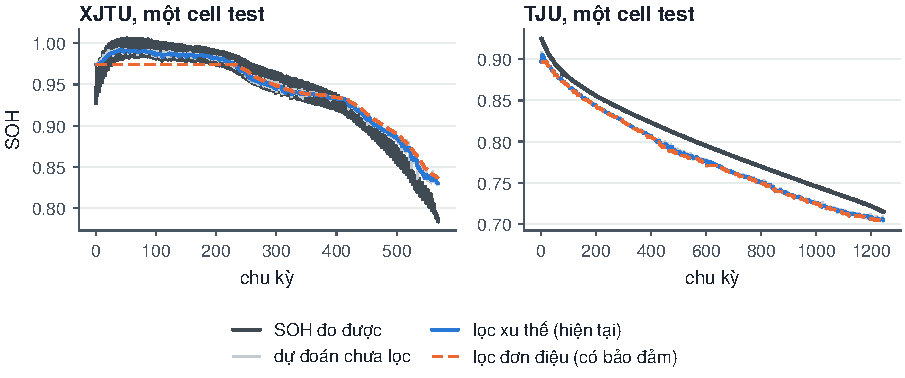
\includegraphics[width=\textwidth]{hinh/fig_mono_example.pdf}
\caption{Một cell test của XJTU có dung lượng tăng đầu đời và một cell TJU (30\,\% nhãn, lần lặp 0): SOH đo được, dự đoán của PINN-lai trước khi lọc, sau bộ lọc xu thế và sau bộ lọc không tăng \eqref{eq:mono} với $(w, a)$ chọn trên validation.}\label{fig:mono}
\end{figure}


\section{Đầu vào có lịch sử của cell}\label{sec:histres}

Dạng lịch sử được chọn ở bước khám phá, trên validation của lần lặp 0 với 30 và 70\,\% nhãn, rồi chốt trước khi chạy
đánh giá cuối. Lịch sử giảm MAE validation của PINN-semi trên XJTU, TJU và HUST (tỉ số 0{,}87--0{,}95) và của GBDT trên XJTU và HUST
(0{,}95--0{,}97); với PINN-semi trên MIT và với GBDT trên TJU và MIT, không có dạng nào đạt ngưỡng 2\,\% nên các mô hình này giữ
đặc trưng gốc. Trên NASA, tính trung bình qua các cách chia, mọi dạng đều kém hơn đặc trưng gốc
(Mục~\ref{sec:nasares}).

\begin{figure}[!htbp]\centering
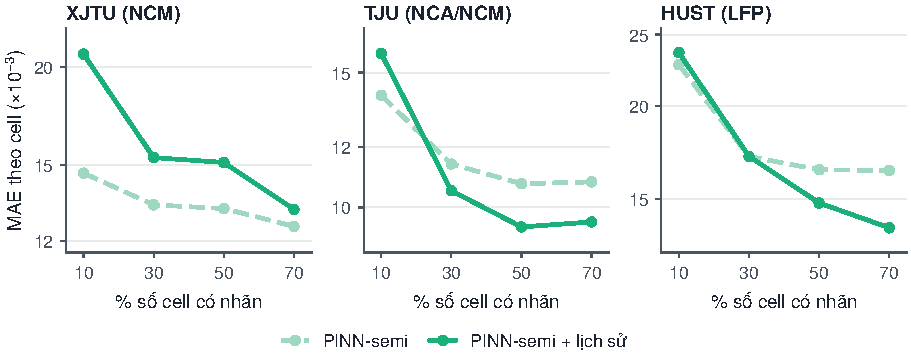
\includegraphics[width=\textwidth]{hinh/fig_e29_pinn.pdf}
\caption{MAE theo cell trên test của PINN-semi không có (nét đứt) và có lịch sử (nét liền), trên ba bộ có dạng lịch sử được chọn; trên MIT không dạng nào được chọn.}\label{fig:e29pinn}
\end{figure}

Trên test (Bảng~\ref{tab:e29}), lịch sử giúp rõ trên TJU và HUST khi có từ 30\,\% nhãn: MAE của PINN-semi còn 0{,}84--1{,}00
lần bản gốc (tốt hơn có ý nghĩa ở 5/6 trường hợp, Hình~\ref{fig:e29pinn}) và của PINN-lai còn 0{,}89--0{,}97 lần (6/6,
Hình~\ref{fig:e29lai}).
Trên XJTU thì ngược lại: PINN-semi có lịch sử kém bản gốc ở mọi mức nhãn (1{,}05--1{,}42 lần), PINN-lai kém 1{,}02--1{,}25 lần. Ở
10\,\% nhãn, lịch sử không giảm sai số có ý nghĩa trên bộ nào (PINN-semi 1{,}04--1{,}42 lần, PINN-lai 0{,}99--1{,}25 lần).

\begin{figure}[!htbp]\centering
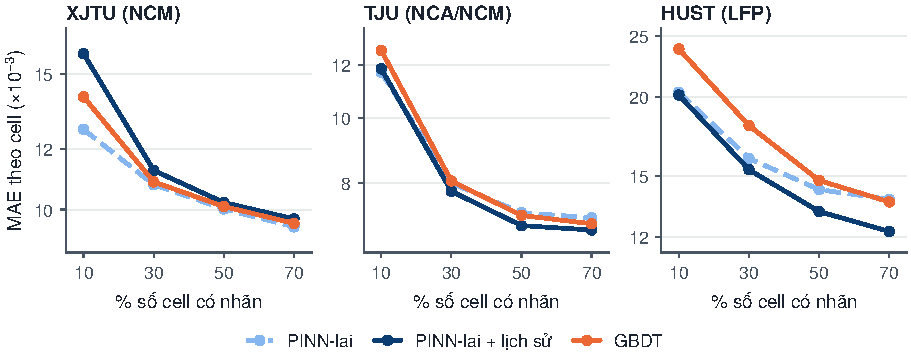
\includegraphics[width=\textwidth]{hinh/fig_e29_lai.pdf}
\caption{MAE theo cell trên test của PINN-lai tinh chỉnh không có (nét đứt) và có lịch sử (nét liền), cạnh GBDT có hoặc không lịch sử chọn trên validation.}\label{fig:e29lai}
\end{figure}

\begin{table}[!htbp]\centering\footnotesize
\caption[MAE theo cell khi có và không có lịch sử]{MAE theo cell ($\times10^{-3}$) trên test, 3 lần lặp $\times$ 5 fold, cùng fold và hạt giống với Mục~\ref{sec:e20res}. PINN-lai là bản tinh chỉnh trên validation (Mục~\ref{sec:tuned}); GBDT là bản có hoặc không lịch sử, chọn trên validation; mô hình cuối là PINN-lai dùng hay không dùng lịch sử theo validation của từng bộ và mức nhãn. $^{*}$/$^{\dagger}$: tốt hơn/kém hơn có ý nghĩa (Wilcoxon ghép cặp theo cell, $p < 0{,}05$) so với cột không lịch sử ngay trước; ở cột cuối, so với GBDT.}\label{tab:e29}
\begin{adjustbox}{max width=\textwidth}\begin{tabular}{llrrrrrr}\toprule
Bộ & Nhãn & PINN-semi & + lịch sử & GBDT & PINN-lai & + lịch sử & Mô hình cuối \\\midrule
XJTU & 10\,\% & 14{,}65 & 20{,}79$^{\dagger}$ & 14{,}01 & 12{,}71 & 15{,}95$^{\dagger}$ & 12{,}71$^{*}$ \\
 & 30\,\% & 13{,}35 & 15{,}34 & 10{,}87 & 10{,}78 & 11{,}25 & 10{,}78$^{*}$ \\
 & 50\,\% & 13{,}20 & 15{,}12 & 10{,}09 & 10{,}02 & 10{,}21 & 10{,}02 \\
 & 70\,\% & 12{,}53 & 13{,}17 & 9{,}60 & 9{,}50 & 9{,}73 & 9{,}50 \\
TJU & 10\,\% & 14{,}01 & 15{,}88$^{\dagger}$ & 12{,}60 & 11{,}70 & 11{,}83 & 11{,}70$^{*}$ \\
 & 30\,\% & 11{,}39 & 10{,}51$^{*}$ & 8{,}06 & 8{,}00 & 7{,}78$^{*}$ & 7{,}78$^{*}$ \\
 & 50\,\% & 10{,}74 & 9{,}43$^{*}$ & 7{,}17 & 7{,}23 & 6{,}92$^{*}$ & 6{,}92$^{*}$ \\
 & 70\,\% & 10{,}80 & 9{,}57$^{*}$ & 6{,}96 & 7{,}11 & 6{,}82$^{*}$ & 6{,}82 \\
MIT & 10\,\% & 3{,}29 & -- & 3{,}15 & 2{,}52 & -- & 2{,}52$^{*}$ \\
 & 30\,\% & 2{,}50 & -- & 1{,}97 & 1{,}75 & -- & 1{,}75$^{*}$ \\
 & 50\,\% & 2{,}45 & -- & 1{,}74 & 1{,}59 & -- & 1{,}59$^{*}$ \\
 & 70\,\% & 2{,}38 & -- & 1{,}59 & 1{,}48 & -- & 1{,}48$^{*}$ \\
HUST & 10\,\% & 22{,}76 & 23{,}63 & 23{,}84 & 20{,}36 & 20{,}15 & 20{,}36$^{*}$ \\
 & 30\,\% & 17{,}10 & 17{,}11 & 18{,}02 & 15{,}99 & 15{,}34$^{*}$ & 15{,}34$^{*}$ \\
 & 50\,\% & 16{,}42 & 14{,}81$^{*}$ & 14{,}75 & 14{,}26 & 13{,}17$^{*}$ & 13{,}17$^{*}$ \\
 & 70\,\% & 16{,}38 & 13{,}71$^{*}$ & 13{,}64 & 13{,}76 & 12{,}24$^{*}$ & 12{,}24$^{*}$ \\
\bottomrule\end{tabular}\end{adjustbox}\end{table}

Lựa chọn ở bước khám phá sai trên XJTU vì nó chỉ dựa trên một lần lặp. Với lần lặp 0, tỉ số MAE validation của
PINN-semi có và không có lịch sử trên XJTU là 0{,}92--0{,}94 ở 30 và 70\,\% nhãn; với lần lặp 2, nó là 1{,}30--1{,}50; trung bình ba
lần lặp là 1{,}06--1{,}17, gần với tỉ số trên test (1{,}06--1{,}15). Mỗi fold của XJTU chỉ có 6 cell validation, nên tác động của lịch sử
đổi theo cách chia cell. Ở 10\,\% nhãn, đầu vào có lịch sử có số chiều gấp đôi đến gấp bốn trong khi chỉ còn vài cell có
nhãn; ngay cả MLP có lịch sử cũng kém MLP gốc 1{,}12--2{,}06 lần ở mức nhãn này.

Validation của đủ ba lần lặp đã có sẵn trong các lượt trên, nên có thể chọn lại mà không dùng test: với mỗi bộ và mức
nhãn, PINN-lai dùng hay không dùng lịch sử, cùng trọng số trộn và cửa sổ lọc, được chọn theo MAE validation trung bình
của 3 lần lặp $\times$ 5 fold; GBDT được chọn có hay không lịch sử theo cùng cách. Bước này được đặt ra sau khi đã thấy
kết quả test ở trên, nên là phân tích hậu kiểm chứ không thuộc đề cương. Validation chọn lịch sử ở TJU và HUST với
30\,\%, 50\,\% và 70\,\% nhãn và bỏ nó ở mọi trường hợp còn lại, trùng với các trường hợp lịch sử có lợi trên test. Với lựa chọn này,
PINN-lai (cột cuối của Bảng~\ref{tab:e29}) có MAE thấp hơn GBDT ở 16/16 trường hợp bộ $\times$ mức nhãn (tỉ số
0{,}80--0{,}99), có ý nghĩa ở 13. Khi GBDT cũng được qua
bộ lọc xu thế với cửa sổ chọn trên validation, tỉ số là 0{,}82--0{,}99, thấp hơn có ý nghĩa ở 11/16 và không trường hợp nào cao hơn có ý nghĩa.

\begin{figure}[!htbp]\centering
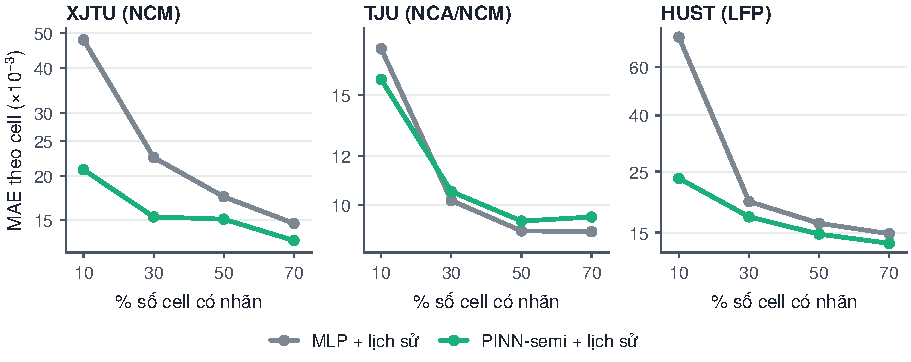
\includegraphics[width=\textwidth]{hinh/fig_e29_phys.pdf}
\caption{MAE theo cell trên test của MLP và PINN-semi khi cả hai cùng có đầu vào lịch sử.}\label{fig:e29phys}
\end{figure}

Ràng buộc vật lý giúp nhiều nhất khi ít nhãn và không giúp ở mọi bộ (Hình~\ref{fig:e29phys}). Khi cả hai cùng có lịch
sử, PINN-semi có MAE bằng 0{,}31--0{,}89 lần MLP ở 10\,\% nhãn, tốt hơn có ý nghĩa trên cả ba bộ. Từ 30\,\% nhãn, tỉ số là 0{,}68--0{,}92 trên XJTU và HUST nhưng
1{,}03--1{,}06 trên TJU, nơi MLP có lịch sử tốt hơn PINN-semi có lịch sử (có ý nghĩa ở 70\,\% nhãn). Không có lịch sử,
TJU cũng như vậy
(1{,}08--1{,}11 ở 50 và 70\,\% nhãn): bộ này gộp ba nhóm hoá học và nhiều nhóm điều kiện, nên một động học dùng chung cho
mọi cell có thể không khớp với từng nhóm.

\section{So với PINN4SOH trên đúng cách chia của bài}\label{sec:paperres}

Bảng~\ref{tab:e27} và Hình~\ref{fig:e27} so mô hình của đồ án với số công bố của PINN4SOH trên đúng các cell test của
bài. Trước hết, bản dựng lại có đáng tin không: PINN động học hộp đen của đồ án, khi dùng bản sao tiền xử lý của bài, có
MAE bằng 0{,}97--1{,}28 lần số công bố, tức cùng cỡ với bài dù cấu hình mạng và lịch học khác. Cùng điều kiện đó, PINN-lai có
MAE bằng 0{,}84--1{,}10 lần PINN4SOH, thấp hơn có ý nghĩa thống kê theo cell trên HUST.

\begin{table}[!htbp]\centering\small
\caption[So với PINN4SOH trên đúng cách chia của bài]{MAE theo cell ($\times10^{-3}$) trên đúng cách chia của PINN4SOH. Hai cột đầu là số công bố của bài; hai cột tiếp theo là mô hình của đồ án với bản sao tiền xử lý của bài (có rò rỉ); ba cột cuối dùng tiền xử lý không rò rỉ của đồ án. Hộp đen: PINN động học hộp đen kiểu PINN4SOH. Trung bình 3 hạt giống, rồi qua các batch như bài.}\label{tab:e27}
\begin{adjustbox}{max width=\textwidth}\begin{tabular}{lrrrrrrr}\toprule
Bộ & PINN4SOH & MLP & Hộp đen & PINN-lai & Hộp đen & GBDT & PINN-lai \\\midrule
XJTU & 7{,}85 & 21{,}02 & 7{,}59 & 6{,}62 & 8{,}32 & 7{,}28 & 7{,}81 \\
TJU & 9{,}79 & 13{,}61 & 10{,}45 & 8{,}78 & 6{,}30 & 6{,}40 & 6{,}16 \\
MIT & 6{,}18 & 7{,}45 & 7{,}88 & 6{,}80 & 2{,}18 & 1{,}44 & 1{,}43 \\
HUST & 7{,}57 & 7{,}77 & 7{,}31 & 6{,}45 & 12{,}60 & 13{,}65 & 12{,}51 \\
\bottomrule\end{tabular}\end{adjustbox}\end{table}


Tiền xử lý của bài vừa thêm một thông tin rò rỉ vừa bỏ đi một thông tin thật, và hai tác động này cân nhau khác nhau theo
bộ. Đổi sang tiền xử lý không rò rỉ, sai số của PINN hộp đen tăng 1{,}10--1{,}72 lần trên XJTU và HUST: chỉ số chu kỳ sau min--max
theo từng cell chính là phần đời đã qua của cell, thông tin mà một mô hình triển khai thật không thể có. Ngược lại, sai
số giảm còn 0{,}28--0{,}60 lần trên TJU và MIT: min--max theo từng cell xoá mức tuyệt đối của đặc trưng sạc, vốn mang thông
tin về SOH. Với tiền xử lý không rò rỉ, PINN-lai có sai số thấp hơn số công bố của PINN4SOH trên TJU và MIT (tỉ số 0{,}23--0{,}63, có ý nghĩa thống kê theo cell trên TJU và MIT), ngang trên XJTU (tỉ số 0{,}99), và chỉ cao hơn trên HUST (tỉ số 1{,}65), đúng bộ mà tiền xử lý của bài có lợi nhất.

\begin{figure}[!htbp]\centering
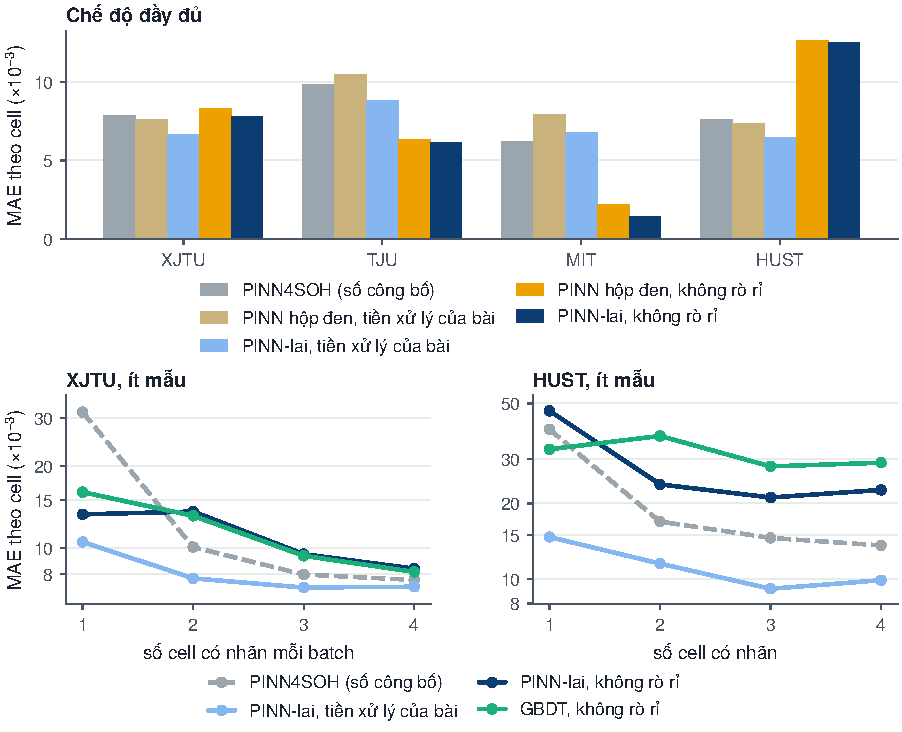
\includegraphics[width=\textwidth]{hinh/fig_e27_compare.pdf}
\caption[So với PINN4SOH trên đúng cách chia của bài]{So với PINN4SOH trên đúng cách chia của bài. Trên: chế độ đầy đủ, mỗi bộ năm cột (số công bố, rồi PINN hộp đen và PINN-lai của đồ án với tiền xử lý của bài và với tiền xử lý không rò rỉ). Dưới: chế độ ít mẫu, MAE theo số cell có nhãn (thang log).}\label{fig:e27}
\end{figure}


Ở chế độ ít mẫu (Hình~\ref{fig:e27}, dưới), với tiền xử lý của bài, PINN-lai có sai số thấp hơn PINN4SOH ở mọi mức $K = 1, \dots, 4$ trên cả XJTU và HUST (tỉ số 0{,}33--0{,}94): các
cell train không nhãn đi vào loss vật lý và bù cho số nhãn ít, rõ nhất khi chỉ một cell có nhãn. Với tiền xử lý không rò
rỉ, PINN-lai chỉ thấp hơn số công bố ở XJTU với $K = 1$ (tỉ số 0{,}42); ở các mức còn lại tỉ số là 1{,}10--1{,}66. Khi chỉ có vài cell có nhãn, biết cell đã đi được bao nhiêu phần đời gần như là biết SOH, nên con số ít
mẫu của bài phần lớn đến từ việc chuẩn hoá theo cả vòng đời cell.

\section{Dự báo SOH tương lai, dung lượng còn lại và RUL}\label{sec:forecastres}

\paragraph{Sai số SOH theo tầm dự báo.} Bảng~\ref{tab:e22soh} cho sai số ở kịch bản
thực tế hơn, khi cell test không được đo dung lượng lần nào và lịch sử SOH là ước lượng PINN-lai. Ba mô hình chỉ dựa
vào lịch sử của chính cell đều kém xa: trên toàn bộ phần đời còn lại, sai số của mô hình kết hợp chỉ bằng
0{,}21--0{,}46 lần sai số của dự báo giữ nguyên, 0{,}39--0{,}60 lần của ngoại suy tuyến tính và 0{,}27--0{,}58 lần của khớp vật lý theo
cell, khác biệt có ý nghĩa trên cả bốn bộ ở cả hai kịch bản. Khớp vật lý theo cell còn kém cả ngoại suy tuyến tính ở XJTU và HUST: ba tham số khớp trên vài trăm điểm có
nhiễu không đủ để phân biệt một quỹ đạo sắp gãy với một quỹ đạo đang chậm dần, đúng nhược điểm đã biết của cách tiếp
cận này. Các mô hình học từ nhiều cell tránh được điều đó vì dạng đường cong được rút ra từ cell khác có đặc trưng
sạc tương tự. Giữa ba mô hình học từ nhiều cell, khác biệt nhỏ hơn nhiều: so với GBDT, mô hình kết hợp có tỉ số sai
số 0{,}91--1{,}06 và tốt hơn có ý nghĩa trên TJU, kém hơn có ý nghĩa trên HUST; so với PINN-dự báo, tỉ số 0{,}88--1{,}00, thấp hơn có ý nghĩa trên XJTU, MIT và HUST. Quy ra dung lượng, sai số của mô hình kết hợp
ở tầm $0{,}5L$ là 20--57 mAh.

\begin{table}[!htbp]\centering\small
\caption[MAE của SOH dự báo ở ba tầm]{MAE theo cell ($\times10^{-3}$) của SOH dự báo ở ba tầm, kịch bản lịch sử ước lượng (không đo dung lượng cell test); in đậm là thấp nhất. Hai cột cuối: mô hình kết hợp khi lịch sử là dung lượng đo, và sai số của mô hình kết hợp quy ra dung lượng (mAh) ở kịch bản ước lượng.}\label{tab:e22soh}
\begin{adjustbox}{max width=\textwidth}\begin{tabular}{llrrrrrrrr}\toprule
Bộ & Tầm & Giữ nguyên & Tuyến tính & Vật lý theo cell & GBDT & PINN-dự báo & Kết hợp & Kết hợp, đo & Kết hợp (mAh) \\\midrule
XJTU & 0{,}1$L$ & 14{,}2 & 12{,}2 & 23{,}4 & \textbf{10{,}8} & 12{,}4 & 10{,}8 & 5{,}4 & 22 \\
 & 0{,}25$L$ & 36{,}2 & 28{,}8 & 39{,}6 & \textbf{16{,}2} & 23{,}5 & 18{,}8 & 13{,}8 & 38 \\
 & 0{,}5$L$ & 70{,}2 & 58{,}8 & 62{,}3 & \textbf{26{,}5} & 32{,}3 & 28{,}4 & 22{,}5 & 57 \\
TJU & 0{,}1$L$ & 15{,}0 & 11{,}0 & 9{,}9 & 9{,}0 & \textbf{8{,}1} & 8{,}4 & 3{,}0 & 29 \\
 & 0{,}25$L$ & 38{,}3 & 23{,}5 & 18{,}5 & 12{,}9 & 13{,}1 & \textbf{12{,}0} & 7{,}2 & 42 \\
 & 0{,}5$L$ & 56{,}5 & 18{,}9 & 17{,}7 & \textbf{10{,}7} & 13{,}0 & 12{,}1 & 11{,}5 & 42 \\
MIT & 0{,}1$L$ & 8{,}9 & 4{,}3 & \textbf{3{,}9} & 5{,}7 & 7{,}2 & 5{,}5 & 4{,}9 & 6 \\
 & 0{,}25$L$ & 26{,}2 & 15{,}3 & 14{,}7 & \textbf{7{,}9} & 10{,}7 & 8{,}8 & 8{,}0 & 10 \\
 & 0{,}5$L$ & 53{,}0 & 39{,}7 & 37{,}6 & \textbf{17{,}0} & 19{,}6 & 17{,}8 & 16{,}8 & 20 \\
HUST & 0{,}1$L$ & 22{,}2 & \textbf{13{,}0} & 35{,}9 & 14{,}3 & 14{,}2 & 13{,}7 & 2{,}8 & 15 \\
 & 0{,}25$L$ & 66{,}3 & 30{,}0 & 103{,}0 & 25{,}4 & 25{,}6 & \textbf{24{,}9} & 8{,}3 & 27 \\
 & 0{,}5$L$ & 136{,}6 & 69{,}1 & 111{,}1 & \textbf{32{,}0} & 37{,}1 & 33{,}1 & 20{,}5 & 36 \\
\bottomrule\end{tabular}\end{adjustbox}\end{table}


\paragraph{Cái giá của việc không đo dung lượng.} Khi lịch sử là dung lượng đo thật, sai số trên toàn bộ phần đời còn
lại bằng 0{,}74; 0{,}63; 0{,}93; 0{,}41 lần sai số khi lịch sử là ước lượng (lần lượt XJTU, TJU, MIT, HUST). Chênh lệch lớn nhất ở HUST,
nơi ở tầm ngắn $0{,}1L$ sai số tăng từ 2{,}8 lên 13{,}7 ($\times10^{-3}$): sai số của dự báo ngắn hạn gần như bằng
sai số ước lượng mức SOH tại gốc, nên chất lượng của mô hình ước lượng quyết định chất lượng dự báo ở tầm ngắn. Ở MIT,
nơi PINN-lai ước lượng SOH rất sát, hai kịch bản gần như trùng nhau. Hình~\ref{fig:e22traj} minh hoạ một cell mỗi bộ:
lịch sử ước lượng, dự báo từ gốc ở 40\,\% đời và khoảng 90\,\%, với trục phải là dung lượng theo Ah.

\begin{figure}[!htbp]\centering
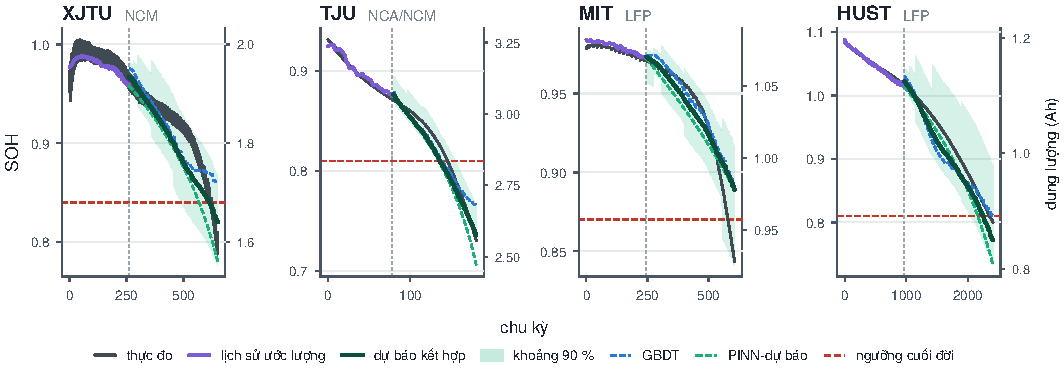
\includegraphics[width=\textwidth]{hinh/fig_e22_traj.pdf}
\caption{Dự báo cho một cell test mỗi bộ (lần lặp 0, gốc ở 40\,\% đời, cell có sai số ở trung vị): lịch sử SOH ước lượng tới gốc, dự báo của GBDT, PINN-dự báo và mô hình kết hợp kèm khoảng 90\,\%; trục phải là dung lượng (Ah).}\label{fig:e22traj}
\end{figure}


\paragraph{RUL.} Bảng~\ref{tab:e22rul} cho thấy khác biệt rõ nhất giữa các mô hình nằm ở
RUL. GBDT không ngoại suy được ra ngoài miền tầm dự báo đã thấy khi học, nên khi RUL dài nó dự báo SOH đi ngang và
cắt ngưỡng quá muộn; sai số RUL của GBDT gấp 1{,}1--1{,}5 lần của mô hình kết hợp, và mô hình kết hợp tốt hơn GBDT có ý
nghĩa trên cả bốn bộ. Nghiệm đóng của PINN-dự báo tiếp tục cong theo hệ số $\lambda$ đã học nên cắt ngưỡng đúng lúc
hơn; giữa mô hình kết hợp và PINN-dự báo, sai số RUL không khác có ý nghĩa trên bộ nào. Như vậy mô hình kết hợp gần bằng GBDT về sai số SOH và
gần bằng PINN-dự báo về RUL, là mô hình duy nhất không kém ở cả hai chỉ số. Tỉ lệ dự báo RUL nằm trong $\pm20\,\%$
RUL thật là 38\,\%; 65\,\%; 48\,\%; 52\,\% và sai số tương đối trung vị 32\,\%; 13\,\%; 21\,\%; 19\,\% (cùng thứ tự bốn bộ); sai số giảm khi gốc dự báo tiến gần
cuối đời, vì phần quỹ đạo còn phải ngoại suy ngắn lại.

\begin{table}[!htbp]\centering\small
\caption[MAE của RUL dự báo]{MAE của RUL (chu kỳ), kịch bản lịch sử ước lượng, trung bình qua gốc ở 25, 50, 75\,\% đời; cột RUL thực là trung bình RUL thật tại các gốc. Ba cột cuối của mô hình kết hợp: MAE khi lịch sử là dung lượng đo, tỉ lệ dự báo nằm trong $\pm20\,\%$ RUL thật và độ phủ thực tế của khoảng RUL 90\,\%.}\label{tab:e22rul}
\begin{adjustbox}{max width=\textwidth}\begin{tabular}{lrrrrrrrrr}\toprule
Bộ & RUL thực & Tuyến tính & Vật lý theo cell & GBDT & PINN-dự báo & Kết hợp & Kết hợp, đo & Trong $\pm20\,\%$ & Độ phủ khoảng \\\midrule
XJTU & 231 & 529 & 499 & 145 & 99 & \textbf{96} & 85 & 38\,\% & 70\,\% \\
TJU & 131 & 50 & 45 & 23 & 23 & \textbf{20} & 14 & 65\,\% & 84\,\% \\
MIT & 344 & 836 & 877 & 131 & 118 & \textbf{113} & 112 & 48\,\% & 67\,\% \\
HUST & 923 & 1354 & 1360 & 312 & \textbf{216} & 218 & 104 & 52\,\% & 65\,\% \\
\bottomrule\end{tabular}\end{adjustbox}\end{table}


\paragraph{Hệ số $\lambda$ học được.} Mạng chỉ thấy đặc trưng tại gốc, không được cho biết bộ dữ liệu, nhưng dấu
của $\lambda$ khớp với hình dạng quỹ đạo của từng bộ. Trung vị $\lambda$ là 3{,}4; −0{,}6; 6{,}7; 4{,}0 (lần lượt XJTU, TJU, MIT, HUST),
với tỉ lệ gốc có $\lambda > 0$ là 83\,\%; 44\,\%; 89\,\%; 100\,\%. Ở XJTU, MIT và HUST, $\lambda$ dương ở phần lớn gốc: tốc độ suy giảm được dự báo tăng dần, đúng với quỹ đạo có điểm đầu gối. Ở TJU, nơi nhiều cell giảm nhanh ở đầu đời rồi chậm lại, trung vị $\lambda$ âm và chỉ khoảng một nửa số gốc có $\lambda > 0$: mạng tự chọn nhánh suy giảm chậm dần của nghiệm đóng. Cùng một dạng phương trình bao được cả hai kiểu quỹ đạo nhờ để dấu của $\lambda$ tự do.

\paragraph{Khoảng dự báo.} Khoảng 90\,\% có độ phủ thực tế 78--84\,\% trên toàn bộ phần đời còn lại và 62--84\,\% với
khoảng RUL, thấp hơn mức đặt ra. Tập validation chỉ có 10\,\% số cell, trong khi sai số dự báo của một cell tương quan
mạnh giữa các tầm; phân vị ước lượng từ vài cell vì vậy hẹp hơn phân bố sai số của cell mới. Khoảng này cho biết bậc
độ lớn của bất định, nhưng chưa đủ tin cậy để dùng như một cam kết 90\,\%.

\section{Dự báo khi dung lượng hồi phục}\label{sec:recoveryres}

Bảng~\ref{tab:e23} so bản dự báo có xét hồi phục với bản ở Mục~\ref{sec:forecastres}, ghép cặp trên cùng gốc. Rõ nhất là
tầm ngắn: với lịch sử đo, trong tầm $0{,}1L$ sau gốc thường, bản mới giảm sai số có ý nghĩa trên XJTU, MIT và HUST (tỉ số 0{,}77--0{,}85), vì
mức xu thế bền xuất phát đúng hơn và GBDT không còn làm lệch đoạn đầu của đường dự báo. Trên toàn bộ phần đời còn lại,
khác biệt nhỏ hơn: tỉ số là 0{,}98--1{,}02 với lịch sử đo và 0{,}95--1{,}04 với lịch sử ước lượng; bản mới tốt hơn có ý nghĩa trên không bộ nào
(lịch sử đo) và trên TJU, MIT và HUST (lịch sử ước lượng), kém hơn có ý nghĩa trên TJU.

Ngay sau một lần hồi phục, bộ lọc quỹ đạo của bản cũ trộn điểm vừa nhảy vào đường hồi quy, nên cú nhảy làm lệch cả mức
lẫn độ dốc của xu thế; bản mới tách cú nhảy khỏi xu thế rồi giữ lại hay bỏ đi theo $\rho$. Trên XJTU, bộ có nhiều gốc
loại này nhất (14 cell), bản mới giảm sai số 5\,\% trên toàn bộ phần đời còn lại (chưa có ý nghĩa thống kê) và 30\,\% trong tầm
ngắn (có ý nghĩa thống kê); trên MIT, tỉ số là 0{,}62 nhưng chỉ có 6 cell nên chưa đủ để kết luận. Trên NASA, tỉ số là 1{,}05
trên toàn bộ phần đời còn lại và 0{,}96 trong tầm ngắn, chưa có ý nghĩa thống kê.

Cặp $(\rho, \tau_r)$ ước lượng trên cell train cho thấy hai kiểu hồi phục: ở XJTU và NASA, phần lớn cú nhảy được giữ lại
(trung vị $\rho$: XJTU 1{,}0, NASA 1{,}0), còn ở MIT, phần hồi phục mất ngay ở chu kỳ sau (MIT $\rho$ = 0{,}0); $\tau_r = $ 0{,}5 chu kỳ
ở mọi bộ, tức không có phần hồi phục tắt dần chậm. Trên NASA, điều này khớp với nhận xét của
SambaMixer~\cite{olalde2024samba} rằng hồi phục gắn với thời gian nghỉ. Dao động đều chỉ được phát hiện ở 22\,\% số gốc
của XJTU, hầu hết thuộc nhóm R2.5. Về RUL, bản mới có sai số thấp hơn có ý nghĩa trên MIT; khoảng 90\,\% có độ phủ 52--84\,\% trên toàn bộ phần đời còn
lại, thấp hơn mức đặt ra vì cùng lý do ở Mục~\ref{sec:forecastres}.

\begin{table}[!htbp]\centering\small
\caption[Dự báo có và không xét hồi phục dung lượng]{MAE theo cell ($\times10^{-3}$) của mô hình kết hợp trên toàn bộ phần đời còn lại, bản E22 và bản có xét hồi phục, ghép cặp trên cùng gốc. Bốn cột đầu: gốc thường, lịch sử ước lượng và lịch sử đo; bốn cột sau: gốc ngay sau một lần hồi phục (lịch sử đo), trên toàn bộ phần đời còn lại và trong tầm $0{,}1L$. $^{*}$/$^{\dagger}$: tốt hơn/kém hơn có ý nghĩa (Wilcoxon ghép cặp theo cell, $p < 0{,}05$); --: không có gốc sau hồi phục.}\label{tab:e23}
\begin{adjustbox}{max width=\textwidth}\begin{tabular}{lrrrrrrrr}\toprule
Bộ & Ước lượng, E22 & Ước lượng, mới & Đo, E22 & Đo, mới & Sau hồi phục, E22 & Sau hồi phục, mới & Ngắn hạn, E22 & Ngắn hạn, mới \\\midrule
XJTU & 22{,}5 & 23{,}0 & 16{,}7 & 16{,}5 & 15{,}4 & 14{,}9 & 6{,}0 & 4{,}2$^{*}$ \\
TJU & 11{,}6 & 11{,}0$^{*}$ & 7{,}3 & 7{,}7$^{\dagger}$ & 26{,}0 & 27{,}7 & 7{,}0 & 7{,}7 \\
MIT & 12{,}0 & 11{,}4$^{*}$ & 11{,}2 & 10{,}7 & 18{,}9 & 10{,}6 & 10{,}1 & 4{,}2 \\
HUST & 27{,}0 & 25{,}7$^{*}$ & 11{,}1 & 11{,}3 & -- & -- & -- & -- \\
NASA & 52{,}6 & 54{,}6 & 23{,}6 & 23{,}5 & 22{,}5 & 23{,}8 & 11{,}2 & 11{,}4 \\
\bottomrule\end{tabular}\end{adjustbox}\end{table}



\section{Bộ dữ liệu NASA}\label{sec:nasares}

\paragraph{Dữ liệu.} 18 cell của NASA chia thành sáu nhóm theo nhiệt độ và chế độ xả (Hình~\ref{fig:nasadata}). Khác
bốn bộ kia, giữa các lần xả có những khoảng nghỉ dài, và dung lượng hồi phục sau đó: sau khoảng nghỉ dưới 10 giờ, SOH
giảm trung vị 0{,}27\,\% so với lần xả trước; sau khoảng nghỉ 10--24 giờ, nó tăng trung vị 0{,}40\,\%; sau khoảng nghỉ
từ 24 giờ trở lên, tăng trung vị 1{,}36\,\%. Đây là các mẫu gây nhiễu mà mọi mô hình phải xử lý khi ước lượng SOH.

\begin{figure}[!htbp]\centering
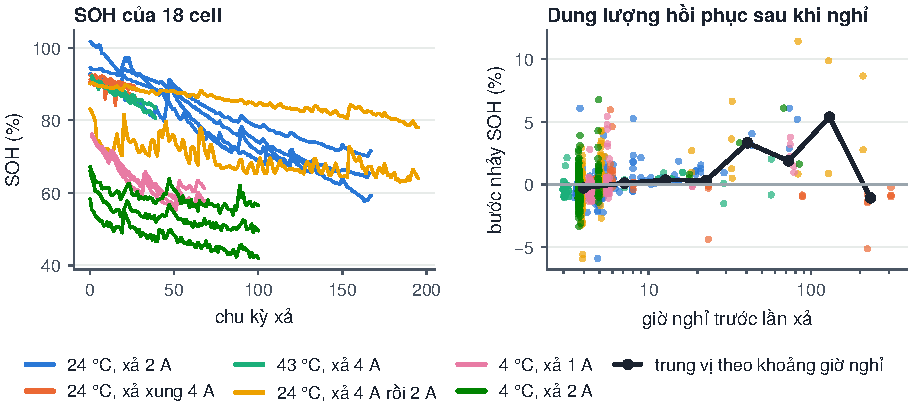
\includegraphics[width=\textwidth]{hinh/fig_nasa_data.pdf}
\caption[Bộ NASA]{Bộ NASA. Trái: SOH theo chu kỳ xả của 18 cell, màu theo nhóm điều kiện thí nghiệm. Phải: thay đổi SOH so với lần xả trước theo thời gian nghỉ trước lần xả (thang log), đường đậm là trung vị theo khoảng.}\label{fig:nasadata}
\end{figure}

\paragraph{Ước lượng SOH.} Bộ NASA được đánh giá bằng đúng giao thức của Chương~\ref{ch:thietke}: kiểm định chéo 5 fold
theo cell, phân tầng theo sáu nhóm giao thức, 3 lần lặp, ở 30 và 70\,\% nhãn (Bảng~\ref{tab:e24cv},
Hình~\ref{fig:nasacompare}). PINN-lai có sai số thấp nhất ở cả hai mức nhãn, 6{,}17\,\% và 5{,}13\,\% SOH. So với MLP,
tỉ số MAE theo cell của nó là 0{,}68 và 0{,}70; so với một PINN-semi là 0{,}79 và 0{,}76 (đều có ý nghĩa thống kê); so
với GBDT là 0{,}96 và 0{,}92, không có ý nghĩa. CNN, LSTM và Transformer có MAE 7{,}86--9{,}18\,\% SOH ở 30\,\% nhãn và 6{,}34--7{,}16\,\% ở 70\,\% nhãn, bằng 0{,}86--1{,}02 lần MLP: cửa sổ nhiều chu kỳ giúp ít hơn so với ở bốn bộ kia, có thể vì dung lượng nhảy lên sau mỗi khoảng nghỉ làm xu thế trong cửa sổ kém ổn định. Sai
số trên NASA lớn hơn nhiều so với bốn bộ kia vì bộ này chỉ có 18 cell trải trên sáu nhóm giao thức và ba mức nhiệt độ:
khi một nhóm chỉ có hai đến bốn cell, cell test thường không có cell train nào cùng điều kiện, và SOH tính theo danh
định 2,0\,Ah của cell 4\,\textdegree C thấp hơn cell 24\,\textdegree C ở cùng số chu kỳ tới 0,4.

\paragraph{Thời gian nghỉ.} Thêm thời gian nghỉ trước lần xả làm đặc trưng thứ 17, theo ý tưởng của
SambaMixer~\cite{olalde2024samba}, không cải thiện có ý nghĩa: tỉ số MAE của PINN-lai có và không có đặc trưng này là
1{,}02 ($p = 0{,}52$) (30\,\% nhãn) và 0{,}98 ($p = 0{,}52$) (70\,\% nhãn). Lý do nằm ở đầu vào. Ở các chu kỳ ngay sau khoảng nghỉ dài (dài hơn hai
lần trung vị của cell), sai số của PINN-lai không lớn hơn các chu kỳ khác (5{,}09 so với 5{,}13\,\% ở 70\,\% nhãn):
đặc trưng sạc được đo sau khoảng nghỉ, nên đã phản ánh trạng thái vừa hồi phục, và thời gian nghỉ không mang thêm thông
tin.

\begin{table}[!htbp]\centering\small
\caption[Bộ NASA, kiểm định chéo theo cell]{Bộ NASA, kiểm định chéo 5 fold theo cell $\times$ 3 lần lặp: MAE theo cell (\% SOH) ở hai mức nhãn, không và có thời gian nghỉ trước lần xả làm đặc trưng thứ 17; in đậm là thấp nhất mỗi cột.}\label{tab:e24cv}
\begin{adjustbox}{max width=\textwidth}\begin{tabular}{lrrrr}\toprule
Mô hình & 30\,\%, 16 đặc trưng & 30\,\%, thêm giờ nghỉ & 70\,\%, 16 đặc trưng & 70\,\%, thêm giờ nghỉ \\\midrule
MLP & 9{,}16 & 10{,}58 & 7{,}03 & 6{,}91 \\
GBDT & 6{,}64 & 6{,}45 & 5{,}73 & 5{,}37 \\
PINN-semi & 7{,}46 & 7{,}56 & 6{,}23 & 6{,}58 \\
3 PINN-semi & 7{,}07 & 7{,}71 & 6{,}10 & 6{,}25 \\
PINN-lai & \textbf{6{,}17} & \textbf{6{,}23} & \textbf{5{,}13} & \textbf{5{,}11} \\
\bottomrule\end{tabular}\end{adjustbox}\end{table}


\paragraph{So với SambaMixer.} Bảng~\ref{tab:e24samba} dùng đúng cách chia NASA-L của SambaMixer: tám cell train, hai cell
giữ lại để dừng sớm, đánh giá trên các cell 6, 7 và 47. PINN-lai có MAE 6{,}78, 3{,}54 và 2{,}05\,\% SOH, cao hơn
SambaMixer trên cả ba cell và chỉ tốt hơn CNN-BiGRU trên cell 47. SambaMixer nhận chuỗi điện áp, dòng điện, nhiệt độ của chính lần xả cần ước lượng; với dòng xả không đổi, thời gian xả
nhân với dòng điện chính là dung lượng, nên nhãn gần như nằm sẵn trong đầu vào. Đồ án dùng đoạn sạc trước lần xả, là
dữ liệu BMS ghi được ở mọi chu kỳ mà không phải xả sâu cell. Sai số lớn nhất ở cell 6 (Hình~\ref{fig:nasatraj}), vốn bắt đầu ở 101\,\% SOH trong khi
các cell train cùng nhóm bắt đầu quanh 92\,\%, với 75--84\,\% số chu kỳ có đặc trưng sạc nằm ngoài miền của cell
train. Trên cùng cách chia, CNN, LSTM và Transformer có MAE trung bình ba cell 5{,}04--7{,}08\,\% SOH, so với 4{,}12\,\% của PINN-lai: nhìn thêm các chu kỳ trước của cell không bù được việc thiếu đường xả của chính chu kỳ cần ước lượng. Đầu vào có lịch sử (Mục~\ref{sec:hist_m}) không được chọn cho NASA: dạng tốt nhất trên validation, tính trung bình qua kiểm định chéo và cách chia NASA-L, vẫn có MAE bằng 1{,}03--1{,}11 lần đặc trưng gốc với PINN-semi và 1{,}27 lần với GBDT. Có thể vì dung lượng NASA nhảy lên sau mỗi lần nghỉ: đặc trưng sạc của chu kỳ hiện tại phản ánh ngay cú nhảy đó, còn trung bình trượt làm nó trễ đi.

\begin{table}[!htbp]\centering\footnotesize
\caption[Cách chia NASA-L của SambaMixer]{Cách chia NASA-L của SambaMixer: MAE (\% SOH) trên ba cell đánh giá. Hai cột đầu lấy từ bài của SambaMixer~\cite{olalde2024samba}, đầu vào là đường xả của chính chu kỳ cần ước lượng; các cột sau là của đồ án, đầu vào là 16 đặc trưng của lần sạc trước đó, trung bình 3 hạt giống.}\label{tab:e24samba}
\begin{adjustbox}{max width=\textwidth}\begin{tabular}{lrrrrrrrr}\toprule
Cell & CNN-BiGRU & SambaMixer-L & MLP & CNN & LSTM & Transformer & GBDT & PINN-lai \\\midrule
B0006 & 2{,}45 & 1{,}17 & 3{,}94 & 4{,}29 & 7{,}25 & 10{,}09 & 10{,}01 & 6{,}78 \\
B0007 & 1{,}86 & 1{,}20 & 4{,}43 & 3{,}44 & 4{,}46 & 4{,}53 & 4{,}48 & 3{,}54 \\
B0047 & 2{,}55 & 0{,}51 & 5{,}55 & 7{,}40 & 7{,}76 & 6{,}63 & 2{,}13 & 2{,}05 \\
Trung bình & 2{,}29 & 0{,}96 & 4{,}64 & 5{,}04 & 6{,}49 & 7{,}08 & 5{,}54 & 4{,}12 \\
\bottomrule\end{tabular}\end{adjustbox}\end{table}

\begin{figure}[!htbp]\centering
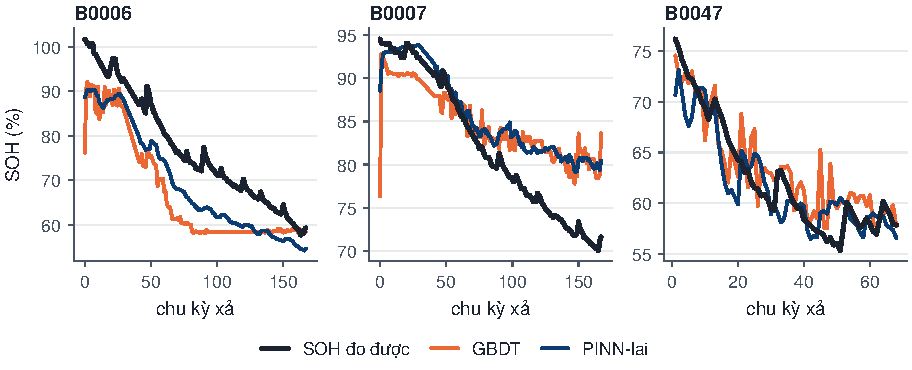
\includegraphics[width=\textwidth]{hinh/fig_nasa_traj.pdf}
\caption{SOH đo được và ước lượng trên ba cell đánh giá của cách chia NASA-L (hạt giống 0, 16 đặc trưng sạc).}\label{fig:nasatraj}
\end{figure}
\begin{figure}[!htbp]\centering
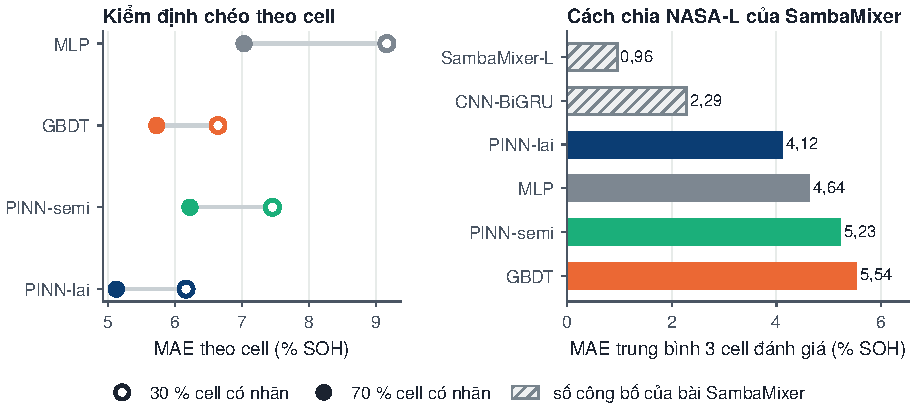
\includegraphics[width=\textwidth]{hinh/fig_nasa_compare.pdf}
\caption[MAE theo cell trên NASA]{MAE theo cell trên NASA. Trái: kiểm định chéo theo cell ở 30\,\% (vòng rỗng) và 70\,\% nhãn (vòng đặc). Phải: trung bình ba cell đánh giá của cách chia NASA-L, cạnh số công bố của bài SambaMixer (gạch chéo).}\label{fig:nasacompare}
\end{figure}


\section{Ngân sách đo dung lượng}\label{sec:budgetres}

\subsection{Đo thưa khi huấn luyện}

Hình~\ref{fig:e28} đặt hai cách gắn nhãn lên cùng một trục: phần trăm số chu kỳ của cell train có đo dung lượng. Gắn
nhãn đầy đủ cho 30\,\% số cell tương ứng 43--44\,\% số chu kỳ train, 70\,\% số cell là toàn bộ. Đo mỗi $0{,}05L$ chu kỳ
trên mọi cell chỉ dùng 1{,}2--6{,}0\,\% số chu kỳ, ít hơn 7--37 lần, nhưng PINN-lai học theo cách này có MAE thấp hơn PINN-lai
học với 30\,\% số cell trên cả bốn bộ (tỉ số 0{,}85--0{,}93, cả bốn có ý nghĩa thống kê; Bảng~\ref{tab:e28}). So với 70\,\% số cell, tỉ số là 0{,}97--1{,}05:
tốt hơn có ý nghĩa ở TJU, kém hơn có ý nghĩa ở MIT, khác biệt không có ý nghĩa ở XJTU và HUST. Khi trọng số trộn và cửa sổ lọc được chọn trên validation cho cả hai cách gắn nhãn (Mục~\ref{sec:tuned},
phân tích hậu kiểm), hai tỉ số này là 0{,}86--0{,}90 và 0{,}99--1{,}05.

\begin{figure}[!htbp]\centering
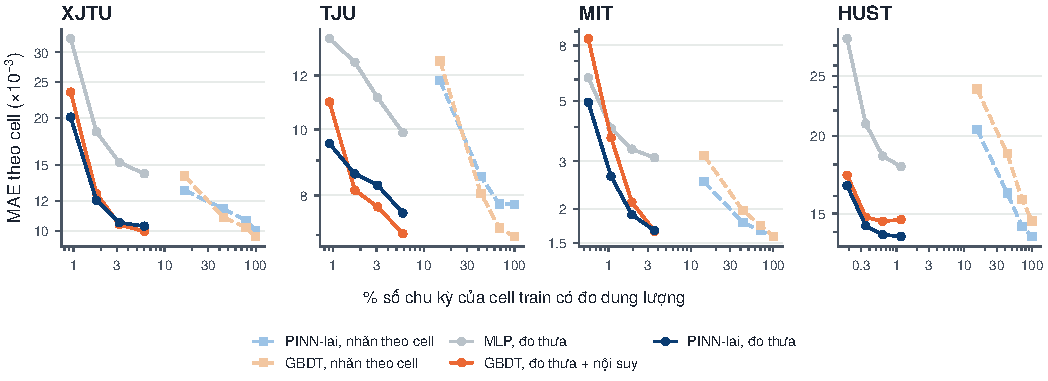
\includegraphics[width=\textwidth]{hinh/fig_e28_budget.pdf}
\caption[MAE theo cell trên test theo phần trăm số chu kỳ của cell train có đo dung lượng (hai trục thang log)]{MAE theo cell trên test theo phần trăm số chu kỳ của cell train có đo dung lượng (hai trục thang log). Nét đứt: nhãn theo cell (10, 30, 50, 70\,\% số cell có nhãn đầy đủ); nét liền: đo thưa mọi cell train theo lịch $qL$, $q$ = 0{,}5; 0{,}2; 0{,}1; 0{,}05.}\label{fig:e28}
\end{figure}


Lợi ích nằm ở chỗ đặt nhãn hơn là ở mô hình. Phần lớn sai số là lệch mức và trôi chậm riêng của từng cell
(Mục~\ref{sec:errdecomp}); mô hình chỉ học được phần này khi thấy nhãn của chính cell đó, trong khi các chu kỳ liền nhau
của một cell gần như lặp lại thông tin của nhau. Đo kín một phần cell dồn công đo vào thông tin lặp lại và bỏ trống độ
lệch của các cell còn lại. Vì vậy GBDT học nhãn nội suy tuyến tính giữa các lần đo ở lịch $0{,}05L$ cũng có sai số
bằng 1{,}00--1{,}04 lần GBDT học với 70\,\% số cell; điều tương tự đúng với mọi mô hình.

Không thành phần nào của PINN-lai tốt nhất ở mọi lịch đo. Ở lịch $0{,}05L$, GBDT học nhãn nội suy tốt hơn trung bình
ba PINN-semi trên cả bốn bộ. Ở lịch thưa nhất ($0{,}5L$, khoảng ba lần đo mỗi cell), nội suy tuyến tính qua nửa đời cell bỏ
qua đoạn suy giảm nhanh về cuối, và GBDT kém hơn ba PINN-semi trên XJTU và MIT (tới 3{,}0 lần); MLP chỉ học trên các lần đo cũng kém ba PINN-semi
1{,}1--2{,}1 lần, vì ràng buộc đơn điệu và động học trên mọi hàng là thứ nối các lần đo với nhau. Trọng số chọn trên validation đi theo lịch đo: $\omega = 0{,}3$ (nghiêng về GBDT) ở lịch $0{,}05L$ trên XJTU, TJU và MIT, $\omega = 0{,}7$ ở lịch $0{,}5L$ trên XJTU và MIT.

\begin{table}[!htbp]\centering\small
\caption[MAE theo cell theo ngân sách đo dung lượng]{MAE theo cell ($\times10^{-3}$) trên test, trung bình 3 lần lặp; trong ngoặc là phần trăm số chu kỳ của cell train có đo dung lượng (70\,\% số cell là toàn bộ). Hai cột đo thưa: mọi cell train được đo ở chu kỳ đầu, sau mỗi $qL$ chu kỳ và ở chu kỳ cuối. Cột cuối: đo thêm cell test theo cùng lịch, cập nhật bằng bộ lọc Kalman, sai số trên các chu kỳ không được đo.}\label{tab:e28}
\begin{adjustbox}{max width=\textwidth}\begin{tabular}{lrrrrrr}\toprule
Bộ & PINN-lai, 30\,\% cell & PINN-lai, 70\,\% cell & GBDT, 70\,\% cell & PINN-lai, đo mỗi $0{,}1L$ & PINN-lai, đo mỗi $0{,}05L$ & đo cả cell mới mỗi $0{,}1L$ \\\midrule
XJTU & 11{,}43 (44{,}1) & 10{,}00 & 9{,}64 & 10{,}51 (3{,}2) & 10{,}28 (6{,}0) & 7{,}46 \\
TJU & 8{,}52 (42{,}6) & 7{,}76 & 6{,}96 & 8{,}28 (3{,}1) & 7{,}54 (5{,}9) & 4{,}13 \\
MIT & 1{,}79 (42{,}7) & 1{,}59 & 1{,}59 & 1{,}91 (1{,}9) & 1{,}67 (3{,}6) & 1{,}18 \\
HUST & 16{,}19 (43{,}1) & 13{,}78 & 14{,}60 & 13{,}87 (0{,}6) & 13{,}78 (1{,}2) & 5{,}00 \\
\bottomrule\end{tabular}\end{adjustbox}\end{table}


\subsection{Đo thưa cả khi dùng}

Khi cell mới cũng được đo theo lịch $0{,}1L$ (1--3\,\% số chu kỳ của nó) và ước lượng được cập nhật bằng bộ lọc Kalman
\eqref{eq:kf}, MAE trên các chu kỳ không được đo của PINN-lai học từ nhãn thưa còn 1{,}2--7{,}5 ($\times10^{-3}$), bằng
0{,}34--0{,}77 lần GBDT học với 70\,\% số cell có nhãn đầy đủ nhưng không đo cell mới. Với cùng lịch đo khi dùng,
PINN-lai học với 70\,\% số cell cho 1{,}0--7{,}4: khi cell mới đã được đo, chênh lệch giữa hai cách huấn luyện không quá
0{,}6 ($\times10^{-3}$).

\subsection{Đo cell mới: một lần lúc nhận hay đo định kỳ}\label{sec:kalmanres}

Với mô hình học từ nhãn theo cell (10--70\,\% cell có nhãn, năm bộ kể cả NASA), đo cell mới mỗi $0{,}1L$ đưa sai số
xuống còn 0{,}33--0{,}72 lần không hiệu chỉnh, mỗi $0{,}25L$ còn 0{,}51--1{,}01 lần. Một lần đo duy nhất lúc nhận pin gần như không giúp (tỉ số
0{,}87--1{,}13) và còn làm kém đi có ý nghĩa ở XJTU và TJU: dung lượng của nhiều cell còn tăng trong vài chục chu kỳ đầu, nên độ lệch
đo ở chu kỳ đầu không đại diện cho về sau. Khi đo dày, dịch ước lượng theo sai số của lần đo gần nhất đã đủ tốt
(hơn bộ lọc có ý nghĩa ở TJU và HUST); bộ lọc có lợi khi đo thưa (mỗi $0{,}25L$, tốt hơn có ý nghĩa trên XJTU, TJU và MIT), vì nó trả độ lệch về mức chung
khi lần đo đã xa. Khoảng 90\,\% của bộ lọc hẹp hơn nhiều so với khoảng phù hợp cố định nhưng độ phủ thực tế chỉ 73--92\,\%.
\section{Thảo luận chung}

Gộp các so sánh chính lại: PINN-lai ở 30\,\% số cell có nhãn có MAE thấp hơn MLP và PINN-semi ở 70\,\% trên cả bốn bộ,
tức kết hợp vật lý, dữ liệu không nhãn và mô hình cây bù được hơn một nửa số cell có nhãn; nhưng nó vẫn kém GBDT ở 70\,\%. Cùng mô hình học từ các lần đo thưa trên mọi cell train (1{,}2--6{,}0\,\% số chu kỳ) có MAE thấp hơn khi
có 30\,\% số cell có nhãn ở cả 20 cặp mô hình và bộ dữ liệu; với mọi mô hình trừ MLP, nó lấy lại ít nhất
59\,\% khoảng cách từ 30\,\% đến 70\,\% số cell có nhãn (Mục~\ref{sec:budgetres}). Câu hỏi đáng đặt ra vì vậy không phải là 30\,\%
nhãn có thắng 70\,\% nhãn hay không, mà là nên đặt các lần đo dung lượng ở đâu.

\paragraph{Khi nào nên dùng PINN bán giám sát?} Giữa các mạng nơ-ron chỉ nhìn một chu kỳ, PINN bán giám sát nên được
dùng thay cho MLP khi số cell có nhãn ít (khoảng 10--30\,\%) và khi có nhiều cell chưa đo dung lượng. Mô hình chuỗi có sai số thấp hơn PINN-semi ở 14/16 trường hợp bằng một con đường khác: nhìn nhiều chu kỳ của chính cell thay vì dùng cell không nhãn (Mục~\ref{sec:dlres}); hai hướng này không loại trừ nhau. So với GBDT
thì khác: trong cùng một bộ dữ liệu, GBDT đơn lẻ có sai số thấp hơn PINN-semi ở phần lớn các trường hợp. Ghép
GBDT với nhóm PINN thì tốt hơn cả hai (Mục~\ref{sec:improve}).

\paragraph{Khi nào lợi ích nhỏ?} Khi đã có đủ nhãn (70\,\%), và trên TJU, nơi tỉ số so với MLP chỉ ở mức 0{,}90--1{,}09 trên mọi mức nhãn. TJU gộp ba nhóm hoá học và chín nhóm điều kiện; có thể biến thiên giữa các nhóm lớn hơn phần mà ràng buộc vật lý dùng chung giải thích được.

\paragraph{Hạn chế.} (i) Khoảng dự báo 90\,\% chưa đạt độ phủ danh nghĩa, và vài lần đo dung lượng chỉ sửa được
mức chứ chưa sửa được hình dạng của quỹ đạo dự báo. (ii) Trọng số vật lý được chọn ở một thí nghiệm sơ bộ và giữ cố định.
(iii) Ràng buộc vật lý chưa được đưa vào chính mô hình cây; PINN-lai chỉ ghép hai mô hình ở mức dự đoán. (iv) Cell validation có nhãn đầy đủ và nằm ngoài ngân sách nhãn ở mọi thí
nghiệm, kể cả khi đo thưa. (v) Ở 30\,\% nhãn, kết luận ở mức fold chỉ vững trên MIT. (vi) Tham số vật lý $\lambda, E_a$ không
được dữ liệu xác định, kể cả khi tăng trọng số ODE (Mục~\ref{sec:physparams}). (vii) Ở dạng đạo hàm riêng, tốc độ $r$ học được không phải tốc độ suy giảm thật của
cell (Mục~\ref{sec:physcheck}). (viii) PINN-lai được
đánh giá với ba lần lặp thay vì năm; quy tắc chọn có hay không lịch sử theo mức nhãn được đặt ra sau khi đã xem test
(Mục~\ref{sec:histres}). (ix) CNN, LSTM, Transformer chỉ được chọn độ dài cửa sổ; kích thước mạng và tốc độ học giữ cố
định, nên sai số của chúng có thể còn giảm khi tinh chỉnh kỹ hơn.

\chapter{Kết luận và hướng phát triển}\label{ch:ketluan}

\section{Kết luận}

Đồ án xây dựng một mô hình PINN bán giám sát cho bài toán ước lượng SOH của cell lithium-ion và đánh giá nó bằng
một giao thức không rò rỉ trên bốn bộ dữ liệu công khai; kiểm toán cho thấy chia theo chu kỳ và chuẩn hoá theo cả vòng
đời cell làm sai số trông thấp hơn thực tế. Trả lời các câu hỏi nghiên cứu:

\begin{enumerate}[label=\textbf{CH\arabic*.}]
\item Cùng 30\,\% nhãn, PINN-semi có sai số thấp hơn MLP có ý nghĩa thống kê trên cả bốn bộ (tỉ số MAE 0{,}76--0{,}96).
\item Lợi ích lớn nhất khi ít nhãn (10\,\%: tỉ số 0{,}39--0{,}90, có ý nghĩa trên cả bốn bộ) và giảm dần khi lượng nhãn tăng.
      Ở 70\,\% nhãn, khi không còn cell không nhãn, cải thiện chỉ còn có ý nghĩa trên MIT, và trên TJU MLP tốt hơn.
\item PINN-semi có MAE thấp hơn MLP trong 14/16, thấp hơn Ridge trong 15/16 và GPR trong 6/16 trường hợp (bộ × mức nhãn), nhưng GBDT tốt hơn PINN-semi trong 14/16 trường hợp, 10 trong đó có ý nghĩa thống kê: trong các mô hình đơn lẻ, GBDT mạnh nhất, trừ trên HUST, nơi các mô hình chuỗi ở CH5 tốt hơn.
\item Ở 10\,\% nhãn, 50--64\,\% mức giảm sai số (thang log) của PINN-semi so với MLP đến từ việc áp loss vật
      lý lên cell không nhãn, phần còn lại từ vật lý trên cell có nhãn. Ở 30\,\% nhãn, riêng ràng buộc đơn điệu đã
      mang lại 62--95\,\% mức giảm đó. Đo trực tiếp trên mô hình đã huấn luyện, vật lý tác động chủ yếu qua
      ràng buộc dọc quỹ đạo (Mục~\ref{sec:physcheck}).
\item Ba mô hình chuỗi (CNN, LSTM, Transformer) có sai số bằng 0{,}36--0{,}93 lần MLP, thấp hơn có ý nghĩa ở 42/48 phép so, nhờ nhìn được nhiều chu kỳ gần nhất của cell; trong ba mô hình, LSTM tốt nhất ở 8/16 trường hợp. Chúng vẫn kém GBDT ở 40/48 và kém PINN-lai ở 47/48 phép so; mô hình cuối có MAE bằng 0{,}77--0{,}96 lần mô hình chuỗi tốt nhất của từng trường hợp, thấp hơn có ý nghĩa ở 14/16.
\item Có. PINN-lai, nhóm ba PINN-semi kết hợp GBDT và bộ lọc quỹ đạo, có MAE thấp hơn PINN-semi ở
      16/16 trường hợp (tỉ số 0{,}67--0{,}95) và thấp hơn GBDT ở 10/16 trường hợp, 8 có ý nghĩa thống kê;
      GBDT chỉ còn tốt hơn có ý nghĩa ở 1 trường hợp.
      Phần lớn lợi ích đến từ việc kết hợp hai mô hình có lệch theo cell chỉ tương quan ở mức vừa; phần vật lý vẫn giúp khi ít
      nhãn (so với cùng công thức dùng MLP, tỉ số 0{,}72 ở 10\,\% nhãn).
\item Có, với độ chính xác giảm dần theo tầm. Khi cell test không được đo dung lượng, mô hình kết hợp
      (PINN-dự báo và GBDT) dự báo SOH trên toàn bộ phần đời còn lại với MAE 11{,}6--27{,}0 ($\times10^{-3}$), bằng 0{,}21--0{,}60
      lần các mô hình chỉ dựa vào lịch sử của chính cell; GBDT gần ngang về SOH nhưng không ngoại suy được ra ngoài
      tầm đã học nên sai số RUL gấp 1{,}1--1{,}5 lần. Khoảng 90\,\% chỉ đạt độ phủ 78--84\,\%. Tách phần hồi phục và dao động đều ra khỏi xu thế giảm sai số tầm ngắn có ý nghĩa trên XJTU, MIT và HUST.
\item Trên đúng cách chia của PINN4SOH, với tiền xử lý không rò rỉ, PINN-lai có sai số bằng 0{,}23--0{,}63 lần số công
      bố trên TJU và MIT, ngang trên XJTU và chỉ kém trên HUST, nơi chỉ số chu kỳ chuẩn hoá theo từng cell cho mô hình của bài biết phần đời đã qua. Cùng tiền xử lý với bài, PINN-lai bằng 0{,}84--1{,}10 lần ở chế độ đầy đủ và 0{,}33--0{,}94 lần ở chế độ
      ít mẫu, nhờ các cell không nhãn đi vào loss vật lý.
\item Nên tính nhãn theo số lần đo dung lượng và rải các lần đo lên mọi cell thay vì đo kín một phần cell. Đo mỗi
      $0{,}05L$ (1{,}2--6{,}0\,\% số chu kỳ train) cho PINN-lai sai số bằng 0{,}85--0{,}93 lần gắn nhãn đầy đủ cho 30\,\% số cell (43--44\,\% số
      chu kỳ) và 0{,}97--1{,}05 lần khi gắn cho 70\,\% số cell; cả năm mô hình đều hưởng lợi theo cùng hướng. Đo thêm cell mới theo lịch $0{,}1L$ và cập nhật bằng bộ lọc Kalman đưa MAE xuống 1{,}2--7{,}5
      ($\times10^{-3}$), bằng 0{,}34--0{,}77 lần GBDT học với 70\,\% cell có nhãn đầy đủ.
\item Lịch sử của cell giúp khi đủ nhãn, nhưng không ở mọi bộ: trên TJU và HUST từ 30\,\% nhãn, nó giảm sai số
      của PINN-lai còn 0{,}89--0{,}97 lần; trên XJTU và ở 10\,\% nhãn thì không. Khi dùng hay không dùng lịch sử được chọn
      trên validation của đủ ba lần lặp (phân tích hậu kiểm), PINN-lai có sai số thấp hơn GBDT ở 16/16 trường hợp
      bộ $\times$ mức nhãn, có ý nghĩa ở 13. Bộ lọc xu thế không bảo đảm SOH không tăng (đầu ra tăng ở 28--44\,\% số bước); ép không tăng làm sai số
      trên XJTU tăng 1{,}8--1{,}9 lần vì dung lượng đo được của XJTU tăng ở đầu đời.
\end{enumerate}

\section{Đối chiếu với đề cương}\label{sec:map}

Bảng~\ref{tab:map} đối chiếu các mục tiêu và nhiệm vụ của giai đoạn 1 trong đề cương với phần đã thực hiện. Đồ án đi
đúng các bước đó, với ba điểm khác về hướng đi. Thứ nhất, đề cương lấy bốn mô
hình học sâu làm mốc so sánh; trên cùng đặc trưng, GBDT có MAE thấp hơn cả bốn ở 12/16 trường hợp bộ
$\times$ mức nhãn (Mục~\ref{sec:dlres}), nên mọi so sánh ở giai đoạn 2 cần có mô hình cây. Thứ hai, thông tin hoá lý
được đưa vào qua hàm mất mát (động học suy giảm có thừa số Arrhenius, tính đơn điệu) và qua bước lọc quỹ đạo, chưa qua
mô hình điện hoá chi tiết; lợi ích của nó rõ nhất khi ít nhãn. Thứ ba, mã hoá vị trí được dùng ở Transformer; mô hình
dự báo có dạng chuỗi sang chuỗi, với mạng mã hoá lịch sử của cell thành tham số và nghiệm đóng của động học sinh quỹ đạo
tương lai; GCN để lại cho bài toán nhiều cell của giai đoạn 2.

\begin{table}[!htbp]\centering\footnotesize
\caption{Đối chiếu mục tiêu và nhiệm vụ của đề cương (giai đoạn 1) với phần đã thực hiện.}\label{tab:map}
\begin{tabularx}{\textwidth}{>{\raggedright\arraybackslash}p{4.6cm}X>{\raggedright\arraybackslash}p{1.9cm}}
\toprule
Đề cương & Đã thực hiện & Mục \\
\midrule
Kiến thức nền: học máy, học sâu cho chuỗi thời gian, dữ liệu pin và ràng buộc hoá lý & MLP, CNN, LSTM, Transformer,
mã hoá vị trí, sequence-to-sequence, GCN; cơ chế suy giảm; PINN & \ref{sec:ts}, \ref{sec:pinn} \\
Tái lập thống kê mô tả; phân tích dữ liệu thô, ngoại lai, mẫu gây nhiễu & Thống kê năm bộ; lọc ngoại lai nhân quả;
hồi phục dung lượng sau khoảng nghỉ của NASA & \ref{sec:data}, \ref{sec:nasares} \\
Chạy và so sánh $\ge 4$ mô hình nền (MLP, CNN, LSTM, Transformer) bằng MAE, RMSE, MAPE & Bốn mô hình nền cùng GBDT,
Ridge, GPR, PINN; MAE, RMSE, MAPE, $R^2$; kiểm định ghép cặp theo cell & \ref{sec:dlres} \\
Tinh chỉnh mô hình, giải thích vì sao tốt lên hay xấu đi & Độ dài cửa sổ; trọng số ghép và cửa sổ lọc; dạng lịch sử;
bộ lọc đơn điệu & \ref{sec:dlres}, \ref{sec:tuned}, \ref{sec:histres}, \ref{sec:monores} \\
Đề xuất cải tiến có cơ sở lý thuyết cho giai đoạn 2 & PINN bán giám sát, PINN-lai, dự báo bằng nghiệm đóng của động học
& \ref{sec:pinn}, \ref{sec:pinnlai_m}, \ref{sec:forecast_m} \\
Xác định phạm vi SOH, RUL; đầu vào, đầu ra, ràng buộc thực tế & Ước lượng SOH trực tuyến từ đoạn sạc; dự báo SOH,
dung lượng, RUL & \ref{sec:forecastres} \\
Thiết kế chỉ số; kịch bản lỗi; phương án dự phòng khi độ tin cậy thấp & MAE theo cell; kiểm toán rò rỉ; khoảng dự
đoán 90\,\%; cập nhật bằng vài lần đo dung lượng & \ref{sec:leakres}, \ref{sec:conformal}, \ref{sec:kalmanres} \\
Bản mẫu, trực quan hoá dữ liệu & Đường ống tái lập được; công cụ dòng lệnh ước lượng và dự báo cho một cell; hình
quỹ đạo & \ref{sec:impl} \\
\bottomrule
\end{tabularx}
\end{table}

\section{Hướng phát triển}

\begin{enumerate}
\item Đưa ràng buộc vật lý vào chính mô hình cây, ví dụ dùng loss đơn điệu và loss động học để tạo nhãn giả cho
      GBDT trên cell không nhãn.
\item Lịch đo chủ động: chọn cell và chu kỳ đo tiếp theo theo độ bất định của mô hình, kiểm chứng trên dữ liệu vận hành thật, nơi các lần đo dung lượng cách nhau không đều.
\item Dùng điện lượng tích luỹ thay cho chỉ số chu kỳ làm biến thời gian, để chuyển giữa các giao thức sạc tốt hơn.
\item Cho $k$ chỉ phụ thuộc vào cell để $\lambda$ và $E_a$ được dữ liệu xác định (Mục~\ref{sec:physparams}).
\item Gắn ràng buộc vật lý vào mô hình chuỗi: dùng LSTM hay Transformer làm mạng nghiệm của PINN, để vừa nhìn được nhiều chu kỳ vừa dùng được cell không nhãn.
\item Giai đoạn 2 của đề cương: mở rộng sang khối pin nhiều cell, mô hình hoá mất cân bằng giữa các cell (chẳng hạn
      bằng GCN trên đồ thị các cell) và dựng giao diện theo dõi từ công cụ dòng lệnh hiện có.
\end{enumerate}

\begin{thebibliography}{99}\small\setlength{\itemsep}{0pt}\setlength{\parsep}{0pt}
\bibitem{angelopoulos2023} A. N. Angelopoulos, S. Bates. Conformal prediction: a gentle introduction.
  \emph{Foundations and Trends in Machine Learning}, 16(4):494--591, 2023.
\bibitem{arlot2010} S. Arlot, A. Celisse. A survey of cross-validation procedures for model selection.
  \emph{Statistics Surveys}, 4:40--79, 2010.
\bibitem{attia2022knee} P. M. Attia, A. Bills, F. Brosa Planella, et al. Review---“Knees” in lithium-ion battery
  aging trajectories. \emph{Journal of The Electrochemical Society}, 169:060517, 2022.
\bibitem{aykol2021} M. Aykol, C. B. Gopal, A. Anapolsky, et al. Perspective---Combining physics and machine
  learning to predict battery lifetime. \emph{Journal of The Electrochemical Society}, 168:030525, 2021.
\bibitem{bai2018tcn} S. Bai, J. Z. Kolter, V. Koltun. An empirical evaluation of generic convolutional and recurrent
  networks for sequence modeling. \emph{arXiv:1803.01271}, 2018.
\bibitem{barlow1972} R. E. Barlow, D. J. Bartholomew, J. M. Bremner, H. D. Brunk. \emph{Statistical Inference under
  Order Restrictions}. Wiley, 1972.
\bibitem{birkl2017} C. R. Birkl, M. R. Roberts, E. McTurk, P. G. Bruce, D. A. Howey. Degradation diagnostics for
  lithium ion cells. \emph{Journal of Power Sources}, 341:373--386, 2017.
\bibitem{bouckaert2004} R. R. Bouckaert, E. Frank. Evaluating the replicability of significance tests for comparing
  learning algorithms. \emph{Advances in Knowledge Discovery and Data Mining (PAKDD)}, 3--12, 2004.
\bibitem{braun2026} C. Braun, J. Raible, M. F. Huber. Physics-informed machine learning in prognostics and health
  management: a systematic literature review. arXiv:2608.10047, 2026.
\bibitem{breiman1996} L. Breiman. Bagging predictors. \emph{Machine Learning}, 24(2):123--140, 1996.
\bibitem{broussely2001} M. Broussely, S. Herreyre, P. Biensan, et al. Aging mechanism in Li ion cells and calendar
  life predictions. \emph{Journal of Power Sources}, 97--98:13--21, 2001.
\bibitem{cleveland1979} W. S. Cleveland. Robust locally weighted regression and smoothing scatterplots.
  \emph{Journal of the American Statistical Association}, 74(368):829--836, 1979.
\bibitem{dietterich1998} T. G. Dietterich. Approximate statistical tests for comparing supervised classification
  learning algorithms. \emph{Neural Computation}, 10(7):1895--1923, 1998.
\bibitem{doyle1993} M. Doyle, T. F. Fuller, J. Newman. Modeling of galvanostatic charge and discharge of the
  lithium/polymer/insertion cell. \emph{Journal of The Electrochemical Society}, 140(6):1526--1533, 1993.
\bibitem{efron1993} B. Efron, R. J. Tibshirani. \emph{An Introduction to the Bootstrap}. Chapman \& Hall, 1993.
\bibitem{fermin2020} P. Fermín-Cueto, E. McTurk, M. Allerhand, et al. Identification and machine learning
  prediction of knee-point and knee-onset in capacity degradation curves of lithium-ion cells. \emph{Energy and AI},
  1:100006, 2020.
\bibitem{friedman2001} J. H. Friedman. Greedy function approximation: a gradient boosting machine.
  \emph{Annals of Statistics}, 29(5):1189--1232, 2001.
\bibitem{grinsztajn2022} L. Grinsztajn, E. Oyallon, G. Varoquaux. Why do tree-based models still outperform deep
  learning on typical tabular data? \emph{Advances in Neural Information Processing Systems}, 35, 2022.
\bibitem{hinton2015} G. Hinton, O. Vinyals, J. Dean. Distilling the knowledge in a neural network.
  arXiv:1503.02531, 2015.
\bibitem{he2011} W. He, N. Williard, M. Osterman, M. Pecht. Prognostics of lithium-ion batteries based on
  Dempster--Shafer theory and the Bayesian Monte Carlo method. \emph{Journal of Power Sources}, 196(23):10314--10321,
  2011.
\bibitem{olalde2024samba} J. I. Olalde-Verano, S. Kirch, C. Pérez-Molina, S. Martín. SambaMixer: State of health
  prediction of Li-ion batteries using Mamba state space models. \emph{IEEE Access}, 2024.
  doi:10.1109/ACCESS.2024.3524321.
\bibitem{hochreiter1997} S. Hochreiter, J. Schmidhuber. Long short-term memory. \emph{Neural Computation},
  9(8):1735--1780, 1997.
\bibitem{holm1979} S. Holm. A simple sequentially rejective multiple test procedure. \emph{Scandinavian Journal of
  Statistics}, 6(2):65--70, 1979.
\bibitem{hu2020joule} X. Hu, L. Xu, X. Lin, M. Pecht. Battery lifetime prognostics. \emph{Joule}, 4(2):310--346,
  2020.
\bibitem{kapoor2023} S. Kapoor, A. Narayanan. Leakage and the reproducibility crisis in machine-learning-based
  science. \emph{Patterns}, 4(9):100804, 2023.
\bibitem{karniadakis2021} G. E. Karniadakis, I. G. Kevrekidis, L. Lu, P. Perdikaris, S. Wang, L. Yang.
  Physics-informed machine learning. \emph{Nature Reviews Physics}, 3:422--440, 2021.
\bibitem{ke2017} G. Ke, Q. Meng, T. Finley, et al. LightGBM: a highly efficient gradient boosting decision tree.
  \emph{Advances in Neural Information Processing Systems}, 30, 2017.
\bibitem{kipf2017} T. N. Kipf, M. Welling. Semi-supervised classification with graph convolutional networks.
  \emph{International Conference on Learning Representations}, 2017.
\bibitem{krishnapriyan2021} A. S. Krishnapriyan, A. Gholami, S. Zhe, R. M. Kirby, M. W. Mahoney. Characterizing
  possible failure modes in physics-informed neural networks. \emph{Advances in Neural Information Processing
  Systems}, 34, 2021.
\bibitem{lakshminarayanan2017} B. Lakshminarayanan, A. Pritzel, C. Blundell. Simple and scalable predictive
  uncertainty estimation using deep ensembles. \emph{Advances in Neural Information Processing Systems}, 30, 2017.
\bibitem{lee2013} D.-H. Lee. Pseudo-label: the simple and efficient semi-supervised learning method for deep neural
  networks. \emph{ICML Workshop on Challenges in Representation Learning}, 2013.
\bibitem{lei2018} J. Lei, M. G'Sell, A. Rinaldo, R. J. Tibshirani, L. Wasserman. Distribution-free predictive
  inference for regression. \emph{Journal of the American Statistical Association}, 113(523):1094--1111, 2018.
\bibitem{loshchilov2019} I. Loshchilov, F. Hutter. Decoupled weight decay regularization. \emph{International
  Conference on Learning Representations}, 2019.
\bibitem{lu2023} J. Lu, R. Xiong, J. Tian, C. Wang, F. Sun. Deep learning to estimate lithium-ion battery state of
  health without additional degradation experiments. \emph{Nature Communications}, 14:2760, 2023.
\bibitem{ma2022} G. Ma, S. Xu, B. Jiang, et al. Real-time personalized health status prediction of lithium-ion
  batteries using deep transfer learning. \emph{Energy \& Environmental Science}, 15:4083--4094, 2022.
\bibitem{nadeau2003} C. Nadeau, Y. Bengio. Inference for the generalization error. \emph{Machine Learning},
  52:239--281, 2003.
\bibitem{navidi2024} S. Navidi, A. Thelen, T. Li, C. Hu. Physics-informed machine learning for battery degradation
  diagnostics: a comparison of state-of-the-art methods. arXiv:2404.04429, 2024.
\bibitem{piombo2024} G. Piombo, S. Fasolato, R. Heymer, et al. Full factorial design of experiments dataset for
  parallel-connected lithium-ion cells imbalanced performance investigation. \emph{Data in Brief}, 53:110227, 2024.
\bibitem{pinson2013} M. B. Pinson, M. Z. Bazant. Theory of SEI formation in rechargeable batteries: capacity fade,
  accelerated aging and lifetime prediction. \emph{Journal of The Electrochemical Society}, 160(2):A243--A250, 2013.
\bibitem{plett2015} G. L. Plett. \emph{Battery Management Systems, Volume I: Battery Modeling}. Artech House, 2015.
\bibitem{raissi2019} M. Raissi, P. Perdikaris, G. E. Karniadakis. Physics-informed neural networks: a deep learning
  framework for solving forward and inverse problems involving nonlinear partial differential equations.
  \emph{Journal of Computational Physics}, 378:686--707, 2019.
\bibitem{rasmussen2006} C. E. Rasmussen, C. K. I. Williams. \emph{Gaussian Processes for Machine Learning}.
  MIT Press, 2006.
\bibitem{richardson2017} R. R. Richardson, M. A. Osborne, D. A. Howey. Gaussian process regression for forecasting
  battery state of health. \emph{Journal of Power Sources}, 357:209--219, 2017.
\bibitem{roman2021} D. Roman, S. Saxena, V. Robu, M. Pecht, D. Flynn. Machine learning pipeline for battery
  state-of-health estimation. \emph{Nature Machine Intelligence}, 3:447--456, 2021.
\bibitem{saxena2008} A. Saxena, J. Celaya, E. Balaban, et al. Metrics for evaluating performance of prognostic
  techniques. In \emph{International Conference on Prognostics and Health Management}, IEEE, 2008.
\bibitem{saha2007nasa} B. Saha, K. Goebel. Battery data set. \emph{NASA Ames Prognostics Data Repository}, NASA
  Ames Research Center, Moffett Field, CA, 2007.
\bibitem{schmalstieg2014} J. Schmalstieg, S. Käbitz, M. Ecker, D. U. Sauer. A holistic aging model for
  Li(NiMnCo)O$_2$ based 18650 lithium-ion batteries. \emph{Journal of Power Sources}, 257:325--334, 2014.
\bibitem{severson2019} K. A. Severson, P. M. Attia, N. Jin, et al. Data-driven prediction of battery cycle life before
  capacity degradation. \emph{Nature Energy}, 4:383--391, 2019.
\bibitem{su2024review} L. Su, Y. Xu, Z. Dong. State-of-health estimation of lithium-ion batteries: a comprehensive
  literature review from cell to pack levels. \emph{Energy Conversion and Economics}, 5(4):224--242, 2024.
\bibitem{sulzer2021} V. Sulzer, P. Mohtat, A. Aitio, et al. The challenge and opportunity of battery lifetime
  prediction from field data. \emph{Joule}, 5(8):1934--1955, 2021.
\bibitem{tarvainen2017} A. Tarvainen, H. Valpola. Mean teachers are better role models: weight-averaged consistency
  targets improve semi-supervised deep learning results. \emph{Advances in Neural Information Processing Systems},
  30, 2017.
\bibitem{thelen2024} A. Thelen, X. Huan, N. Paulson, S. Onori, Z. Hu, C. Hu. Probabilistic machine learning for
  battery health diagnostics and prognostics---review and perspectives. \emph{npj Materials Sustainability}, 2:14,
  2024.
\bibitem{varma2006} S. Varma, R. Simon. Bias in error estimation when using cross-validation for model selection.
  \emph{BMC Bioinformatics}, 7:91, 2006.
\bibitem{vovk2005} V. Vovk, A. Gammerman, G. Shafer. \emph{Algorithmic Learning in a Random World}. Springer, 2005.
\bibitem{vaswani2017} A. Vaswani, N. Shazeer, N. Parmar, et al. Attention is all you need. \emph{Advances in Neural
  Information Processing Systems}, 30, 2017.
\bibitem{waldmann2014} T. Waldmann, M. Wilka, M. Kasper, M. Fleischhammer, M. Wohlfahrt-Mehrens. Temperature
  dependent ageing mechanisms in lithium-ion batteries -- a post-mortem study. \emph{Journal of Power Sources},
  262:129--135, 2014.
\bibitem{wang2011lfp} J. Wang, P. Liu, J. Hicks-Garner, et al. Cycle-life model for graphite-LiFePO$_4$ cells.
  \emph{Journal of Power Sources}, 196(8):3942--3948, 2011.
\bibitem{wang2021grad} S. Wang, Y. Teng, P. Perdikaris. Understanding and mitigating gradient flow pathologies in
  physics-informed neural networks. \emph{SIAM Journal on Scientific Computing}, 43(5):A3055--A3081, 2021.
\bibitem{wang2024} F. Wang, Z. Zhai, Z. Zhao, Y. Di, X. Chen. Physics-informed neural network for lithium-ion
  battery degradation stable modeling and prognosis. \emph{Nature Communications}, 15:4332, 2024.
\bibitem{wen2023} P. Wen, Z.-S. Ye, Y. Li, S. Chen, P. Xie, S. Zhao. Physics-informed neural networks for
  prognostics and health management of lithium-ion batteries. arXiv:2301.00776, 2023.
\bibitem{wilcoxon1945} F. Wilcoxon. Individual comparisons by ranking methods. \emph{Biometrics Bulletin},
  1(6):80--83, 1945.
\bibitem{wolpert1992} D. H. Wolpert. Stacked generalization. \emph{Neural Networks}, 5(2):241--259, 1992.
\bibitem{zhang2018lstm} Y. Zhang, R. Xiong, H. He, M. G. Pecht. Long short-term memory recurrent neural network for
  remaining useful life prediction of lithium-ion batteries. \emph{IEEE Transactions on Vehicular Technology},
  67(7):5695--5705, 2018.
\bibitem{zhang2023batteryml} H. Zhang, et al. BatteryML: an open-source platform for machine learning on battery
  degradation. \emph{arXiv:2310.14714}, 2023.
\bibitem{zhu2022} J. Zhu, Y. Wang, Y. Huang, et al. Data-driven capacity estimation of commercial lithium-ion
  batteries from voltage relaxation. \emph{Nature Communications}, 13:2261, 2022.
\end{thebibliography}
\end{document}
